\documentclass[10pt]{book}
\usepackage{huy,math,titlepage,code}
\theoremstyle{definition}
\newtheorem{exercise}{Exercise}[chapter]
\newtheorem{example}{Example}[chapter]
\newenvironment{solution}{\begin{proof}}{\end{proof}}
\pagestyle{headings}
\usepackage[margin=2cm]{geometry}
%===============
\author{Huy Bui}
\title{CCNA notebook}
\date{\today}
\begin{document}
\titleAT{CCNA}
\thispagestyle{empty}{\tableofcontents}

\part{NETWORK FUNDAMENTALS}
\chapter{Seven layers}

\section{Introductions}

A group of inter-related protocols necessary to perform a communication function is called a \textbf{protocol suite}.The \textbf{TCP/IP protocol suite} is an open standard, meaning these protocols are freely available to the public, and any vendor is able to implement these protocols on their hardware or in their software. The TCP/IP protocol suite includes many protocols, as shown in Figure \ref{TCPIP}.

\begin{figure}[hbtp]
\caption{TCP/IP protocol suite and Communication process}\label{TCPIP}
\centering
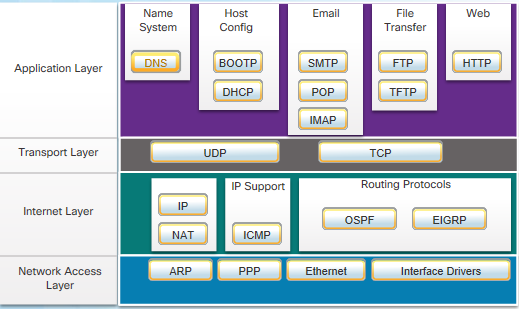
\includegraphics[scale=0.7]{pictures/TCPIP.PNG}
\end{figure}

Figure \ref{ProtocolEncap}  demonstrate the complete protocol encapsulation during the \textbf{TCP/IP communication process}. The process begins with the web server preparing the HTML page as \emph{data} to be sent. The application protocol \emph{HTTP} header is added to the front of the HTML data. The transport layer divides a data stream into segments and may add reliability and flow control information (TCP). Next, the Layer 3 (network layer) adds IP addresses and control information to each segment to create packets. Then, Layer 2 (Data Link layer) protocol (Ethernet, PPP, HDLC, etc.) adds information to both ends of the IP packet, known as a data link frame. This data is now ready to be transported through the internetwork via Layer 1 (Physical layer).\\

\begin{figure}[hbtp]
\caption{Protocol encapsulation}\label{ProtocolEncap}
\centering
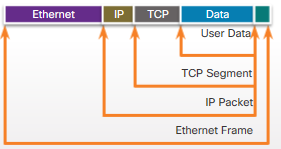
\includegraphics[scale=0.8]{pictures/ProtocolEncap.PNG}
\end{figure}

Whereas the TCP/IP model layers (table \ref{TCP}) are referred to only by name, the seven OSI model layers (table \ref{OSI}) are more often referred to by number rather than by name. For instance, the physical layer is referred to as Layer 1 of the OSI model.

\tableStart[\caption{The OSI Reference Model}\label{OSI}] {|c|l|p{12cm}|}
\head{Number} & \head{Layer} & \head{Description} \w
7 & Application & contain protocols used for process-toprocess communications\w
6 & Presentation & provide for common representation of the data transferred between application layer services\w
5 & Session & organize dialog and manage data exchange\w
4 & Transport & segment, transfer, and reassemble\w
3 & Network & exchange the individual pieces of data over the network \w
2 & Data Link & exchange data frames between devices over a common media\w
1 & Physical & describe the mechanical, electrical media to create physical connections for bit transmission\w
\tableEnd

\tableStart[\caption{The TCP/IP Reference Model}\label{TCP}] {|c|p{12cm}|}
\head{Layer} & \head{Description} \w
Application & represent data to user plus encoding and dialog control\w
Transport & support communication between various devices across diverse networks\w
Internet & determine best path through the network \w
Network Access & control hardware devices and media\w
\tableEnd

\section{Physical layer}

\subsection{Introduction}

The OSI physical layer provides the means to transport the bits that make up a data link layer frame across the network media. This layer accepts a complete frame from the data link layer and encodes it as a series of signals that are transmitted onto the local media.\\

The physical layer standards address three functional areas:

\begin{itemize}
\item \textbf{Physical Components:} electronic hardware devices, media, and other connectors that transmit and carry the signals to represent the bits.

\item \textbf{Encoding:} a method of converting a stream of data bits into a predefined code. Codes are groupings of bits used to provide a predictable pattern that can be recognized by both the sender and the receiver. 

\item \textbf{Signaling:} The physical layer must generate the electrical, optical, or wireless signals that represent the 1 and 0 on the media. The method of representing the bits is called the \emph{signaling method}. A common signaling method  is using modulation techniques. \emph{Modulation} is the process by which the characteristic of one wave (the signal) modifies another wave (the carrier).
\end{itemize}

\textbf{Bandwidth} is the capacity of a medium to carry data. Digital bandwidth measures the amount of data that can flow from one place to another in a given amount of time in kb/s, Mb/s, and Gb/s. A combination of factors determines the practical bandwidth of a network: The properties of the physical media, The technologies chosen for signaling and detecting network signals.\\

\textbf{Throughput} is the measure of the transfer of bits across the media over a given period of time. Due to a number of factors, throughput usually does not match the specified bandwidth in physical layer implementations. Many factors influence throughput, including: The type and amount of traffic and Latency\footnote{Latency refers to the amount of time, to include delays, for data to travel from one given point to another.} between source and destination. \emph{Throughput cannot be faster than the slowest link in the path from source to destination}. \\

There are three basic forms of network media: Copper cable (electrical pulses), fiber optic (light), and wireless (microwave transmissions).\\

\subsection{Copper cable}

Copper cable is inexpensive and easy to install but limited by distance and signal interference. There are two sources of signal interference:

\begin{itemize}
\item \textbf{EMI or RIF:} distort and corrupt the data signals; potential source: radio waves, electromagnetic devices, such as fluorescent lights or electric motors. To counter the negative effects of EMI and RFI, some types of copper cables are wrapped in metallic shielding and require proper grounding connections.

\item \textbf{Crosstalk} is a disturbance caused by the electric or magnetic fields of a signal on one wire to the signal in an adjacent wire. To counter the negative effects of crosstalk, some types of copper cables have opposing circuit wire pairs twisted together. 
\end{itemize}

There are three main types of copper media used in networking:

\begin{itemize}
\item \textbf{Unshielded Twisted-Pair (UTP):} These cables are used to interconnect nodes on a LAN and infrastructure devices such as PCs, switches, routers. UTP cabling, terminated with \textbf{RJ-45} connectors, consists of \textbf{four} pairs of color-coded wires that have been twisted together. 

\item \textbf{Shielded twisted-pair (STP)} provides better noise protection than UTP cabling.

\item \textbf{Coaxial cable} contains two conductors that share the same axis. 
\end{itemize}

\tableStart[\caption{UTP Categories}\label{UTPcat}] {|l|l|}
\head{Category} & \head{Speed} \w
Cat3 Cable (UTP) & 10Mb/s\w
Cat5 & 100 -- 1000 Mb/s\w
Cat5e& 1000 Mb/s \w
Cat6 &  1000 Mb/s -- 10 Gb/s \w
\tableEnd

\tableStart[\caption{Copper cable types}] {|l|p{4cm}|p{10cm}|}
\head{UTP cable} & \head{Standard} & \head{Application} \\
Straight-through & Both ends T568A or T568B & PC to switch, switch to router \w
Crossover & One end T568A, the other end T568B & switch to switch, router to router, PC to router \w
Rollover & Cisco proprietary & Connects a workstation serial port to a router console port \w
\tableEnd

\subsection{Fiber optic}

Optical fiber cable transmits data over longer distances and at higher bandwidths than any other networking media. Unlike copper wires, fiber-optic cable can transmit signals with less attenuation and is completely immune to EMI and RFI. 

\tableStart[\caption{Fiber Cable Components}]{|l|p{12cm}|}
\head{Component} & \head{Description} \w
Core & The core is actually the light transmission element at the center of the optical fiber. This core is typically silica or glass. Light pulses travel through the fiber core.\w
Cladding & It tends to act like a mirror by reflecting light back into the core of the fiber. This keeps light in the core as it travels down the fiber.\w
Buffer & Used to help shield the core and cladding from damage.\w
Strengthening material & Surrounds the buffer, prevents the fiber cable from being stretched when it is being pulled. The material used is often the same material used to produce bulletproof vests.\w
Jacket & a PVC jacket that protects the fiber against abrasion, moisture, and other contaminants.\w
\tableEnd

Light pulses representing the transmitted data as bits on the media are generated by either Lasers or LEDs. Fiber-optic cables are broadly classified into two types:

\begin{itemize}
\item \textbf{Single-mode fiber (SMF)} consists of a very small core and uses \emph{laser} to send a \emph{single} ray of light. Popular in long-distance situations spanning hundreds of kilometers: long-haul telephony, cable TV, campus backbones .

\item \textbf{Multimode fiber (MMF)} consists of a larger core and uses LED emitters to send light pulses. It provides bandwidth up to 10 Gb/s over link lengths of up to 550 meters.

\item One of the highlighted differences between multimode and single-mode fiber is the amount of \emph{dispersion}. Dispersion refers to the spreading out of a light pulse over time. The more dispersion there is, the greater the loss of signal strength.
\end{itemize}

\subsection{Wireless}

Wireless media provides the greatest mobility options of all media. Wireless does have some areas of concern, including Coverage area, Interference, Security, and Shared medium. There are many types of wireless media: WiFi (IEEE 802.11 standard), Bluetooth  (IEEE 802.15 standard), and Wi Max (IEEE 802.16 Standard).

\section{Data Link layer}

The PDU of Data Link layer is always \textbf{frame}. The data link layer is divided into two sublayers: Logical Link Control (LLC) and Media Access Control (MAC). See Figure \ref{Sublayers}.

\subsection{Logical Link Control sublayer (LLC)}

This upper sublayer communicates with the network layer. It places information in the frame that identifies which network layer protocol is being used for the frame. This information allows multiple Layer 3 protocols, such as IPv4 and IPv6, to utilize the same network interface and media.\\

\begin{figure}[hbtp]
\caption{Data Link sublayers}\label{Sublayers}
\centering
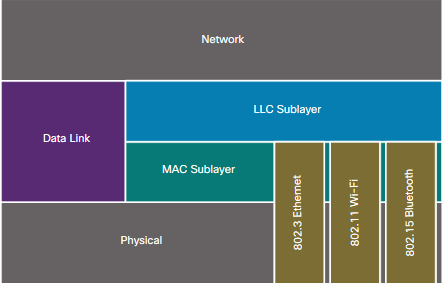
\includegraphics[scale=0.7]{pictures/Sublayers.PNG}
\end{figure}

LLC is implemented in software, and its implementation is independent of the hardware. In a computer, the LLC can be considered the driver software for the NIC. The NIC driver is a program that interacts directly with the hardware on the NIC to pass the data between the MAC sublayer and the physical media.

\subsection{Ethernet MAC sublayer}

The Ethernet MAC sublayer has two primary responsibilities: Data encapsulation and Media Access Control. \\

The \textbf{data encapsulation} process includes frame assembly before transmission and frame disassembly upon reception of a frame. Data encapsulation provides three primary functions: Frame delimiting, Addressing, and Error detection. \\

\textbf{Media access control} is responsible for the placement of frames on the media and the removal of frames from the media. As its name implies, it controls access to the media. This sublayer communicates directly with the physical layer. The actual media access control method used depends on Topology and Media sharing.\\

\paragraph{Multi-access networks} Ethernet LANs\footnote{Various hosts connect to a single switch (or hub) using Ethernet cables.} and WLANs\footnote{Various hosts connect to an access point via radio transmissions} are examples of a multiaccess network. At any one time, there may be a number of devices attempting to send and receive data using the same network media. Therefore, multi-access networks require rules to govern how devices share the physical media. Those rules, together, form a media access control method. There are two basic access control methods for shared media:

\begin{itemize}
\item \textbf{Contention-based access:} All nodes operating in half-duplex compete, only one device can send at a time. Ethernet LANs \emph{using hubs} and WLANs are examples of this type of access control.

\item \textbf{Controlled access:} Each node has its own time to use the medium, a device must wait its turn to access the medium. Legacy Token Ring LANs are an example of this type of access control. 
\end{itemize}

\note Ethernet LANs using \emph{switches} do not use a contention-based system because the switch and the host NIC operate in full-duplex mode.\\

The \textbf{CSMA/CD} (Carrier Sense Multiple Access/Collision Detection) process is used in \emph{half-duplex Ethernet LANs}. A PC's NIC needs to determine if anyone is transmitting on the medium. If it does not detect a carrier signal or receives transmissions from another device, it will assume the network is available to send. If another device wants to transmit, it must wait until the channel is clear. Additionally, CSMA/CD stops transmitting when congestion occurs. It also uses a random time to re-sent a frame.\\

The \textbf{CSMA/CA} (Carrier Sense Multiple Access/Collision Avoidance) process is used in \emph{WLAN}. CSMA/CA does not detect collisions but attempts to avoid them by waiting before transmitting. Each device that transmits includes the time duration that it needs for the transmission. All other wireless devices receive this information and know how long the medium will be unavailable. 

\subsection{Frame}

\subsubsection{Generic Frame}

The data link layer prepares a packet for transport across the local media by encapsulating it with a header and a trailer to create a frame. Each frame has three parts: Header, Data, and Trailer (Figure \ref{Frame}). The generic frame field types include:

\begin{figure}[hbtp]
\caption{Frame fields}\label{Frame}
\centering
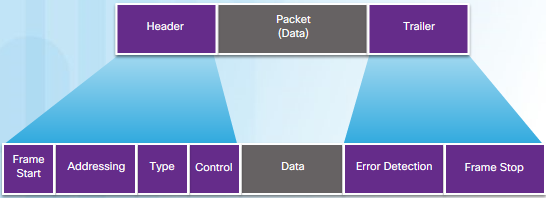
\includegraphics[scale=0.8]{pictures/Frame.PNG}
\end{figure}


\begin{itemize}
\item \textbf{Frame start and stop indicator flags} identify the beginning and end limits of the frame.

\item \textbf{Addressing} indicates the source and destination nodes on the media.

\item \textbf{Type} identifies the Layer 3 protocol in the data field.

\item \textbf{Control} identifies special flow control services such as quality of service (QoS). 

\item \textbf{Data} contains the frame payload 

\item \textbf{Error Detection}
\end{itemize}

The trailer is used to determine if the frame arrived without error. This process is called error detection. Cyclic Redundancy Check (CRC) value is placed in the Frame Check Sequence (FCS) field to represent the contents of the frame. In the Ethernet trailer, the FCS checks transmission errors.\\

\begin{figure}[hbtp]
\caption{Layer 2 Data Link addresses change at each point along the way}\label{Frame2}
\centering
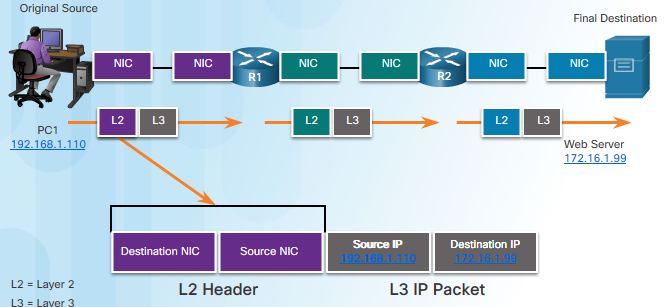
\includegraphics[ width=0.8\textwidth ]{pictures/Frame2.PNG}
\end{figure}

As the IP packet travels from host-to-router, router-to-router, and finally router-to-host, at each point along the way the IP packet is encapsulated in a new data link frame (Figure \ref{Frame2}). Each data link frame contains the source data link address of the NIC card sending the frame and the destination data link address of the NIC card receiving the frame. Remember that the data link layer address is only used for local subnet delivery. 

\subsubsection{Ethernet Frame}

\paragraph{Size} The minimum Ethernet frame size is 64 bytes and the maximum is 1518 bytes\footnote{ The Preamble field is not included when describing the size of a frame.}. Any frame less than 64 bytes in length is called a \emph{collision fragment} or \emph{runt frame}. Frames with more than 1500 bytes of data are called \emph{jumbo frames} or \emph{baby giant frames}. If the size of a transmitted frame is less than the minimum or greater than the maximum, the receiving device drops the frame. 

\paragraph{Frame fields} The \emph{Preamble} (7 bytes) and \emph{Start Frame Delimiter} (1 byte) fields are used for synchronization between the sending and receiving devices. The \emph{Type} field (2 bytes) identifies the upper layer protocol in hexadecimal: IPv4 = 0x800, IPv6 = 0x86DD, ARP = 0x806.

\paragraph{Ethernet MAC addresses}(6 bytes) are made up of two parts: vendor code OUI (3 bytes) assigned by IEEE and device identifier (3 bytes). When the computer starts up, the first thing the NIC does is copy the MAC address from ROM into RAM. \textbf{Broadcast MAC} address is \textbf{FF-FF-FF-FF-FF-FF} (twelve F letters). The \textbf{multicast MAC} address associated with an IPv4 multicast address is a special value that begins with \textbf{01-00-5E} in hexadecimal. The remaining portion of the multicast MAC address is created by converting the lower 24 bits of the IP multicast group address into 6 hexadecimal characters. For an \textbf{IPv6} address, the multicast MAC address begins with \textbf{33-33}.



\subsection{ARP}

To determine the destination MAC address, the device uses ARP. ARP provides two basic functions: Resolving IPv4 addresses to MAC addresses, Maintaining a table of mappings. \\

When a packet is sent to the data link layer to be encapsulated into an Ethernet frame, the device refers to a table in its memory to find the MAC address that is mapped to the IPv4 address. This table is called the ARP table or the ARP cache. The ARP table is stored in the RAM of the device. \\

The sending device will search its ARP table for a destination IPv4 address and a corresponding MAC address. If the destination IPv4 address is on the \emph{same} network as the source IPv4 address, the device will search the ARP table for the destination IPv4 address. Otherwise, the device will search the ARP table for the IPv4 address of the default gateway.\\

For each device, an ARP cache timer removes ARP entries that have not been used for a specified period of time. The times differ depending on the device's operating system. For example, Windows store ARP cache entries for 2 minutes.\\

\paragraph{ARP request} If there is no entry is found in ARP table for a particular IPv4 address, then the device sends an ARP request. ARP messages are encapsulated directly within an Ethernet frame. There is no IPv4 header (Figure \ref{ARPrequest}). Destination MAC address is a broadcast address. ARP messages have a type field of \textbf{0x806}. 

\tableStart[\caption{ARP request message}\label{ARPrequest}] {|c|c|c|c|}
Destination MAC & Source MAC & \textbf{Target} IPv4 & Target MAC \w
FF-FF & 00-0A & 192.68.1.5 & -- \w
\tableEnd

\paragraph{ARP reply} Only the device with an IPv4 address associated with the target IPv4 address in the ARP request will respond with an ARP reply. Only the device that originally sent the ARP request will receive the unicast ARP reply. The ARP reply is encapsulated in an Ethernet frame (Table \ref{ARPreply}).

\tableStart[\caption{ARP request message}\label{ARPreply}] {|c|c|c|c|}
Destination MAC & Source MAC & \textbf{Sender} IPv4 & Sender MAC \w
00-0A & 00-0B & 192.68.1.5 & 00-0B \w
\tableEnd

\paragraph{ARP broadcasts}  If a large number of devices were to be powered up, and all start sending ARP requests, there could be some reduction in performance for a short period of time. 

\paragraph{ARP spoofing} is a technique used by an attacker to reply to an ARP request for an IPv4 address belonging to another device, such as the default gateway. The attacker sends an ARP reply with its own MAC address. The receiver of the ARP reply will add the wrong MAC address to its ARP table and send these packets to the attacker.

\section{Network layer}

Network Layer PDU Is an \textbf{Packet}.

\subsection{Introduction}

The network layer has four basic processes: Addressing end devices, routing, encapsulation, de-encapsulation. There are several network layer protocols in existence, but there are only two network layer protocols that are commonly implemented: \textbf{IPv4} and \textbf{IPv6}.\\

IP encapsulates the transport layer segment or other data by adding an IP header. This header remains the same from the time the packet leaves the source host until it arrives at the destination host.\\

The protocols in network layer were not designed to track and manage the flow of packets. The basic characteristics of IP are

\begin{itemize}
\item \textbf{Connectionless:} no dedicated end-to-end connection is created before data is sent. 
\item \textbf{Best Effort:} The IP protocol does not guarantee that all packets that are received. Furthermore, IP is unreliable which means that IP does not have the capability to manage and recover from undelivered or corrupt packets
\item \textbf{Media Independent:} Operation is independent of the medium (i.e., copper, fiber optic, or wireless) carrying the data.
\end{itemize}

There is, however, one major characteristic of the media that the network layer considers: \textbf{MTU} (maximum transmission unit). The data link layer passes the MTU value up to the network layer. The network layer then determines how large packets can be.\\

Sometimes, a IPv4 router must split up a packet when forwarding it from one medium to another medium with a smaller MTU. This process is called \textbf{fragmentation}. Unlike IPv4, IPv6-enabled routers do not fragment packets.

\subsection{Packet header}

Significant fields in the \textbf{IPv4} header include (Figure \ref{IPv4packet}):

\begin{itemize}
\item \textbf{Version:} is set to \textbf{0100} that identifies this as an IP version 4 packet.

\item \textbf{DiffServ:} used by QoS service to determine the priority.

\item \textbf{TTL:} limit the lifetime of a packet. The value is decreased by one each time the packet is processed by a router. If the TTL field decrements to zero, the router discards the packet and sends an \emph{ICMP Time Exceeded} message to the source IP address.

\item \textbf{Protocol:} identify the next level protocol. Common values include \textbf{ICMP (1)}, \textbf{TCP (6)}, and \textbf{UDP (17)}.

\item \textbf{Source IPv6 Address}

\item \textbf{Destination IPv6 Address}
\end{itemize}

\begin{figure}[hbtp]
\caption{IPv4 packet header}\label{IPv4packet}
\centering
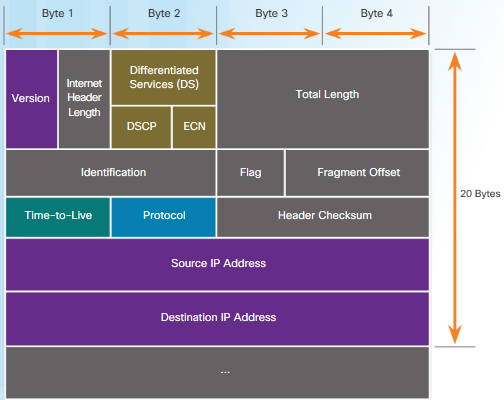
\includegraphics[scale=0.6]{pictures/IPv4packet.PNG}
\end{figure}

Significant fields in the \textbf{IPv6} header include (Figure \ref{IPv6packet}):

\begin{itemize}
\item \textbf{Version:} is set to \textbf{0110} that identifies this as an IP version 6 packet.

\item \textbf{Traffic class:} equivalent to the IPv4 DiffServ field.

\item \textbf{Payload Length:} indicates the length of the data portion of the packet.

\item \textbf{Hop Limit:} equivalent to the IPv4 TTL field.

\item \textbf{Next Header:} equivalent to the IPv4 Protocol field.
\end{itemize}

\subsection{Routing table}

When a router interface (g0/0) is configured with an IPv4 address (192.168.10.1), a subnet mask (255.255.255.0), and is activated, the following two routing table entries are automatically created:

\begin{verbatim}
C 192.168.10.0/24 is directly connected, GigabitEthernet0/0
L 192.168.10.1/32 is directly connected, GigabitEthernet0/0
\end{verbatim}

The letter \textbf{C} identifies a directly connected \emph{network}. The letter \textbf{L} shows that this is a local interface and its IP address is 192.168.10.1.\\

The routing table also stores information about remote network. For example, the entry for the remote network 10.1.1.0 is as follows:

\begin{verbatim}
D 10.1.1.0/24 [90/2170112] via 209.165.200.226, 00:00:09, Serial0/0/0
\end{verbatim}

The details of the remote network routing table entry are explained as follow:

\begin{itemize}
\item \verb|D| -- Identifies how the network was learned by the router. Common  route sources include \textbf{S} (static route), \textbf{D} (EIGRP), \textbf{O} (OSPF).

\item \verb|10.1.1.0/24| -- Identifies the destination network.

\item \verb|90| -- Identifies the AD of the route.

\item \verb|2170112| -- Identifies the metric of the route.

\item \verb|209.165.200.226| -- Identifies the IP address of the router to forward the packet.

\item \verb|00:00:09| -- Router timestamp

\item \verb|Serial0/0/0| -- Identifies the exit interface to use to forward a packet
\end{itemize}

\subsection{Router Boot-up}

This topic will introduce the structure of Cisco routers and how they boots up.\\

A Cisco router has four types of memory:

\begin{itemize}
\item \textbf{RAM:} This is volatile memory that stores: IOS image, Running configuration file, Routing table, ARP cache, and Packet buffer.

\item \textbf{ROM:} This non-volatile memory is used to store Bootstrap program, Power-on self-test (POST), and Limited IOS (backup IOS).

\item \textbf{NVRAM:} This non-volatile memory is used to store Startup configuration file.

\item \textbf{Flash:} This non-volatile computer memory used as permanent storage for the IOS and other system-related files (log, HTML files, etc.) When a router is rebooted, the IOS is copied from flash into RAM.
\end{itemize}

\begin{figure}[hbtp]
\caption{Cisco router bootup process}\label{BootUp}
\centering
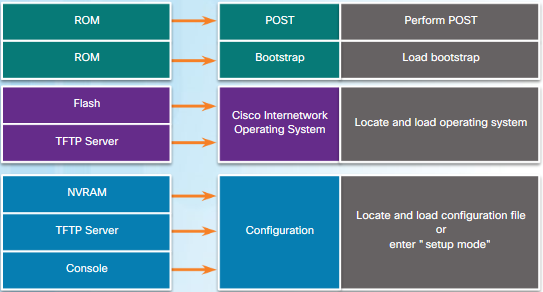
\includegraphics[ width=0.7\textwidth ]{pictures/BootUp.PNG}
\end{figure}

There are three major phases to the bootup process, as shown in Figure \ref{BootUp}.

\begin{enumerate}
\item \textbf{POST process and Bootstrap Program:} During the Power-On Self-Test (POST), the router executes diagnostics on hardware components (CPU, RAM, NVRAM, etc.). After the POST, the bootstrap program is copied from ROM into RAM.

\item \textbf{Loading Cisco IOS:} The IOS image is copied from Flash memory into RAM. If the image is not located in flash, then the router may look for it using a TFTP server. If a full IOS image cannot be located, a Limited IOS (in ROM) is copied into RAM, which can be used to diagnose problems and transfer a full IOS into Flash memory.

\item \textbf{Loading the Startup configuration File:} The bootstrap program then copies the startup configuration file from NVRAM into RAM. This becomes the running configuration. If the startup configuration file does not exist in NVRAM, the router may be configured to search for a TFTP server. If a TFTP server is not found, then the router displays the setup mode prompt.
\end{enumerate}

\note Setup mode is not used in this course to configure the router. When prompted to enter setup mode, always answer no. If you answer yes and enter setup mode, press Ctrl+C at any time to terminate the setup process.\\

Use \verb|show version| to check the version of the Cisco IOS, the version of the bootstrap program, and information about the hardware configuration, including the amount of system memory.

\subsection{Router configuration}

\tableStart[\caption{Initial router configuration}] {|l|l|}
\head{Task} & \head{Commands}\w
Configure the device name & \verb|hostname BranchRouter| \w

Secure user EXEC mode & 
\begin{minipage}{4in}
\begin{verbatim}
line console 0
  password cisco12345
  login
\end{verbatim} 
\end{minipage} \w

Secure remote Telnet/SSH access & 
\begin{minipage}{4in}
\begin{verbatim}
line vty 0 4
  password cisco12345
  login
\end{verbatim} 
\end{minipage} \w

Secure privilege EXEC mode & \verb|Router(config)# enable secret password|\w

Secure all passwords & \verb|Router(config)# service password-encryption|\w

Provide legal notification & \verb|Router(config)# banner motd "message"|\w

Save the configuration & \verb|Router# copy run start|\w

Configure the interface & 
\begin{minipage}{3in}
\begin{verbatim}
interface s0/0/0
  ip address 192.168.100.1 255.255.255.0
  description Connect to R1
  no shutdown
\end{verbatim}
\end{minipage}\w

Verify interface configuration & 
\begin{minipage}{3in}
\begin{verbatim}
show interface
show ip interface
show ip interface brief
show ip route
\end{verbatim}
\end{minipage}\w

\tableEnd

\section{Transport layer}

The PDU of transport layer is either \textbf{segment} or \textbf{datagram}. The transport layer is responsible for:

\begin{itemize}
\item Establishing a temporary communication session between two applications and delivering data between them. 
\item Tracking individual conversations
\item Segmenting data and Reassembling segments
\item To pass data streams to the proper applications, transport layer assigns each application an identifier called a \textbf{port number}. 
\end{itemize}

\subsection{TCP}

TCP is considered a reliable, full-featured transport layer protocol, which ensures that all of the data arrives at the destination. However, this requires additional fields in the TCP header which increases the size of the packet and also increases delay. With TCP, there are three basic operations of reliability:

\begin{itemize}
\item Numbering and tracking data segments transmitted 
\item Acknowledging received data
\item Retransmitting any unacknowledged data 
\end{itemize}

TCP has the following features:

\begin{itemize}
\item  \textbf{Connection-oriented:} TCP negotiates and establishes a virtual connection between source and destination devices prior to forwarding any traffic.

\item \textbf{Reliable:} TCP ensures that each segment arrives at the destination. 

\item \textbf{Stateful protocol:} A stateful protocol is a protocol that keeps track of the state of the communication session. 

\item \textbf{Same-Order Delivery:} Because networks may provide multiple routes that can have different transmission rates, data can arrive in the wrong order. By numbering and sequencing the segments, TCP can ensure that these segments are reassembled into the proper order.

\item \textbf{Flow control:} When TCP is aware that these resources are overtaxed, it can request that the sending application reduce the rate of data flow. To accomplish this, the TCP header includes a field called the \emph{window size}.
\end{itemize}

\begin{figure}[hbtp]
\caption{TCP segment}\label{TCPheader}
\centering
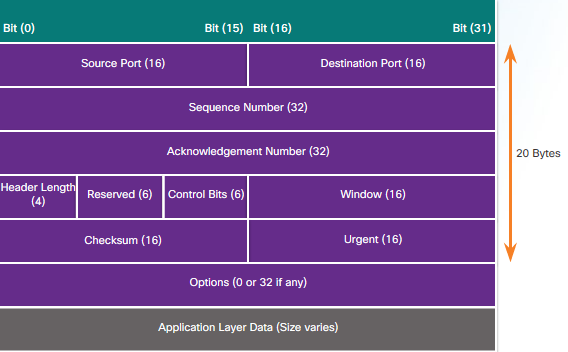
\includegraphics[scale=0.5]{pictures/TCPheader.PNG}
\end{figure}


Each TCP segment has 20 bytes of overhead (Figure \ref{TCPheader}) in the header encapsulating the application layer data:

\begin{itemize}
\item \textbf{Source Port and Destination Port}

\item \textbf{Sequence number} –- Used for data reassembly purposes. During session setup, an \textbf{initial sequence number (ISN)} is set. ISN is the starting value of Sequence number. As data is transmitted during the session, the sequence number is incremented. 

\item \textbf{Acknowledgement number} – Indicates the data that has been received. Acknowledgement number sent back to the source to indicate the next byte that the receiver expects to receive. This is called \emph{expectational acknowledgement}. When TCP at the source host has not received an acknowledgement after a predetermined amount of time, it returns to the last ACK number received and retransmits the data from that point forward. 

\item \textbf{Header length} -– Indicates the length of the TCP segment header.
\item \textbf{Reserved} -– This field is reserved for the future.
\item \textbf{Control bits} -– Known as flags, these identify bit codes that indicate the purpose and function of the TCP segment.
\item \textbf{Window size} -– Indicates the number of bytes that can be accepted at one time. The window size is included in every TCP segment, so the destination can modify the window size at any time depending on buffer availability. The initial window size is agreed upon  TCP three-way handshake. 
\item \textbf{Checksum} -– Used for error checking of the segment header and data.
\item \textbf{Urgent} -– Indicates if data is urgent.
\end{itemize}

A TCP connection is established in three-way handshake:

\begin{enumerate}
\item The client requests a client-to-server communication session with the server
\item The server acknowledges the client-to-server communication session and requests a server-to-client communication session
\item The client acknowledges the server-to-client communication session 
\end{enumerate}

The TCP connect is terminated in \textbf{two} two-way handshakes with four exchanges:

\begin{enumerate}
\item When the client has no more data to send in the stream, it sends a segment with the FIN flag set 
\item The server sends an ACK to acknowledge the receipt of the FIN to terminate the session from client to server. So step 1 and 2 is the first two-way handshake
\item The server sends a FIN to the client to terminate the server-to-client session
\item The client responds with an ACK to acknowledge the FIN from the server
\end{enumerate}

TCP is a \textbf{full-duplex} protocol, where each connection represents two one-way communication sessions. To establish the connection, the hosts perform a \textbf{three-way handshake}. Control bits in the TCP header indicate the progress and status of the connection. 

\subsection{UDP}

UDP is a lightweight transport protocol that offers the same data segmentation and reassembly as TCP, but without TCP reliability and flow control. It is known as a \textbf{best-effort} delivery protocol. UDP is also a \textbf{stateless} protocol, meaning neither the client, nor the server, is obligated to keep track of the state of the communication session.\\

\begin{figure}[hbtp]
\caption{UDP datagram}\label{UDPheader}
\centering
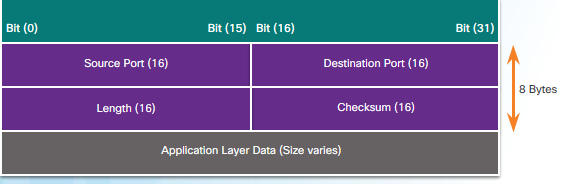
\includegraphics[scale=0.5]{pictures/UDPheader.PNG}
\end{figure}


UDP has no way to reorder the datagrams into their transmission order. Therefore, UDP simply reassembles the data in the order that it was received and forwards it to the application. \\

The pieces of communication in UDP are called datagrams. These datagrams are sent as best-effort by the transport layer protocol. UDP has a low overhead of 8 bytes (Figure \ref{UDPheader}).

There are three types of applications that are best suited for UDP:

\begin{itemize}
\item Live video and multimedia applications (e.g. VoIP, live streaming video)
\item Simple request and reply applications (e.g. DNS\footnote{DNS can also use TCP if the DNS request or DNS response is more than 512 bytes}, DHCP)
\item Applications that handle reliability themselves (SNMP\footnote{SNMP uses UDP by default, but it can also use TCP}, TFTP)
\end{itemize}

\subsection{Port number}

The source port number is associated with the originating application on the local host. The destination port number is associated with the destination application on the remote host. Each application process running on the server is configured to use a port number. An individual server cannot have two services assigned to the same port number within the same transport layer services.\\

The combination of the source IP address and source port number, or the destination IP address and destination port number is known as a socket. The socket is used to identify the server and service being requested by the client. In figure \ref{Socket}, the client socket is 192.168.1.5:1099 with 1099 representing the source number, the socket on the web server is 192.168.1.7:80. Together, these two sockets combine to form a socket pair: 192.168.1.5:1099, 192.168.1.7:80 \\

\begin{figure}[hbtp]
\caption{Examples of socket pairs}\label{Socket}
\centering
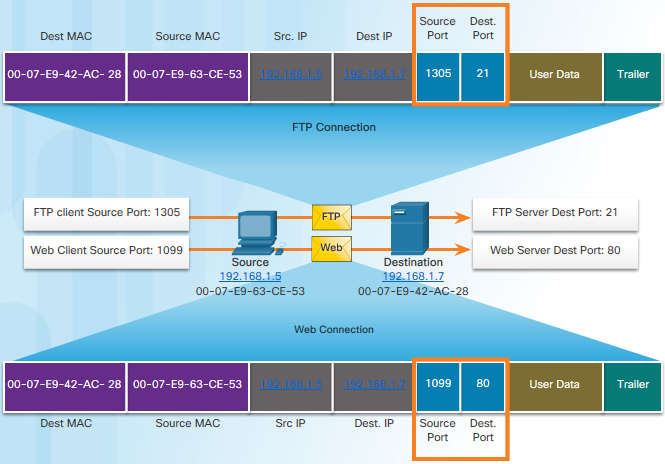
\includegraphics[ width=0.7\textwidth ]{pictures/Socket.PNG}
\end{figure}

There are different types of port numbers:

\begin{itemize}
\item \textbf{Well-known Ports} (0 -- 1023): These numbers are used for popular applications such as FTP, HTTP, TFTP, etc.

\item \textbf{Registered Ports} (1024 -- 49151): These port numbers are assigned by IANA to a requesting entity to use with specific processes or applications.

\item \textbf{Dynamic or Private Ports} (49152 -- 65535): These are assigned dynamically by the client's OS to identify the application during communication.
\end{itemize}

\tableStart[\caption{Protocol port number}] {|l|l|l|}
\head{Port number} & \head{Protocol} & \head{Application}\w
20 & TCP & FTP (data)\w
21 & TCP & FTP (client)\w
22 & TCP & SSH\w
23 & TCP & Telnet\w
25 & TCP & SMTP\w
53 & UDP, TCP & DNS\w
67, 68 & UDP & DHCP\w
69 & UDP & TFTP\w
80 & TCP & HTTP\w
443 & TCP & HTTPS\w
110 & TCP & POP3\w
143 & TCP & IMAP\w
161 & UDP & SNMP\w
\tableEnd

\section{Application layer}

The PDU of application layer is \textbf{data}.  Application layer protocols are used to exchange data between programs running on the source and destination hosts. The upper three layers of the OSI model (application, presentation, and session) define functions of the single TCP/IP application layer.

\subsection{Presentation and Session Layer}

The presentation layer has three primary functions: Formatting, Compressing, and Encrypting. Specifically, it formats data for the application layer, and it sets standards for file formats (QuickTime, MPEG, GIF, PNG, JPEG, etc.).\\

Functions at the session layer create and maintain dialogs between source and destination applications. The session layer handles the exchange of information to initiate dialogs, keep them active, and to restart sessions that are disrupted or idle for a long period of time.\\

\subsection{Peer-to-peer network}

In the peer-to-peer (P2P) networking model, the data is accessed from a peer device without the use of a dedicated server. The P2P network model involves two parts: P2P networks and P2P applications. Every connected end device (known as a peer) can function as both a server and a client. \\

With P2P applications, each computer in the network running the application can act as a client or a server for the other computers in the network running the application. Common P2P networks include: eDonkey, G2, BitTorrent, Bitcoin. Some P2P applications are based on the Gnutella protocol, where each user shares whole files with other users. 

\subsection{HTTP}

When a web address or URL (uniform resource locator) is typed into a web browser, the web browser establishes a connection to the web service running on the server using the HTTP protocol. URLs and URIs (Uniform Resource Identifier) are the names most people associate with web addresses.\\

HTTP is a request/response protocol. When a client sends a request to a web server, HTTP specifies the message types used for that communication. The three common message types are GET (A client request for data), POST (Upload data files), and PUT (Upload resources or content).\\

\textbf{HTTPS} uses the same client request-server response process as HTTP, but the data stream is encrypted with Secure Socket Layer (SSL) before being transported across the network.

\subsection{Email}

Email is a \emph{store-and-forward} method of sending, storing, and retrieving electronic messages across a network. Email messages are stored in databases on mail servers. An email client does not communicate directly with another email client when sending email. Instead, both clients rely on the mail server to transport messages. \\

Email supports three separate protocols for operation: SMTP, POP3, IMAP. The application layer process that sends mail uses SMTP. A client retrieves email using one of the two application layer protocols: POP or IMAP.\\

SMTP port is \textbf{25}. \\

When the server receives the message, it either places the message in a local account (if the recipient is local) or forwards the message to another mail server for delivery. The destination email server may not be online or may be busy when email messages are sent. Therefore, SMTP spools messages to be sent at a later time. Periodically, the server checks the queue for messages and attempts to send them again. If the message is still not delivered after a predetermined expiration time, it is returned to the sender as undeliverable. \\

\paragraph{POP3} is used to retrieve mail from a mail server. With POP, by default, mail is downloaded from the server to the client and then deleted on the server. 

\paragraph{IMAP} is another protocol that describes a method to retrieve email messages. Unlike POP, when the user connects to an IMAP-capable server, copies of the messages are downloaded to the client application.  The original messages are kept on the server until manually deleted. With IMAP, users can create a file hierarchy on the server to organize and store mail. That file structure is duplicated on the email client as well. When a user decides to delete a message, the server synchronizes that action and deletes the message from the server.

\subsection{DNS}

In data networks, devices are labeled with numeric IP addresses to send and receive data over networks. Domain names were created to convert the numeric address into a simple, recognizable name. For example, a domain name, such as \verb|http://www.cisco.com|, is much easier for people to remember than 198.133.219.25, which is the actual numeric address for this server. \\

The DNS (Domain Name Service)  defines an automated service that matches resource names with the required numeric network address. The steps involved in DNS resolution are as follows:

\begin{enumerate}
\item User enters a fully qualified domain name (FQDN).
\item The client computer  sends a DNS query to the DNS server requesting an IP address to match the FQDN
\item The DNS server resolve the FQDN to an IP address in the DNS server database
\item The DNS server sends back a response to the client with the IP address for the FQDN
\end{enumerate}

The DNS server stores different types of resource records used to resolve names. These records contain the name, address, and type of record. Some of these record types are:

\begin{itemize}
\item A – An end device IPv4 address
\item NS – An authoritative name server
\item AAAA – An end device IPv6 address (pronounced quad-A)
\item MX – A mail exchange record
\end{itemize}

When a client makes a query, the server's DNS process first looks at its own records to resolve the name. If it is unable to resolve the name using its stored records, it contacts other servers to resolve the name. After a match is found and returned to the original requesting server, the server temporarily stores the numbered address in the event that the same name is requested again. The DNS Client service on Windows PCs also stores previously resolved names in memory. The \code{ipconfig /displaydns} command displays all of the cached DNS entries.\\

\begin{figure}[hbtp]
\caption{A hierarchy of DNS server}\label{DNSprocess}
\centering
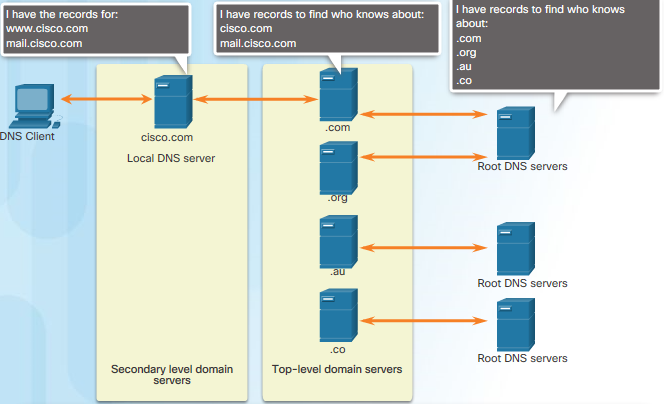
\includegraphics[ width=0.8\textwidth ]{pictures/DNSprocess.PNG}
\end{figure}


The DNS protocol uses a hierarchical system to create a database to provide name resolution (Figure \ref{DNSprocess}). The naming structure is broken down into small, manageable zones. Each DNS server maintains a specific database file and is only responsible for managing name-to-IP mappings for that small portion of the entire DNS structure.\\

The different top-level domains represent either the type of organization or the country of origin. Examples of top-level domains are: .com (business or industry), .org (non-profit organization), .fi (Finland), etc.\\

Computer operating systems also have a utility called \emph{nslookup} that allows the user to manually query the name servers to resolve a given host name. This utility can also be used to troubleshoot name resolution issues and to verify the current status of the name servers. When the nslookup command is issued, the default DNS server configured for your host is displayed. 

\subsection{FTP}

FTP transfers data between a client and a server. To successfully transfer data, FTP requires two connections between the client and the server, one for commands and replies, the other for the actual file transfer:

\begin{itemize}
\item The \textbf{client} establishes the first connection to the server for control traffic using \textbf{TCP} port \textbf{21}, consisting of client \emph{commands} and server \emph{replies}.

\item The client establishes the second connection to the server for the \emph{actual data transfer} using \textbf{TCP} port \textbf{20}. This connection is created every time there is data to be transferred. The data transfer can happen in either direction. The client can download (pull) data from the server, or the client can upload (push) data to the server.
\end{itemize}

\subsection{SMB}

The Server Message Block (SMB) is a client/server file sharing protocol that describes the structure of shared network resources, such as directories, files, printers, and serial ports. It is a request-response protocol. SMB messages can

\begin{itemize}
\item Start, authenticate, and terminate sessions
\item Control file and printer access
\item Allow an application to send or receive messages to or from another device
\end{itemize}

Microsoft support SMB file-sharing. Unlike the file sharing supported by FTP, clients establish a long-term connection to servers. After the connection is established, the user of the client can access the resources on the server as if the resource is local to the client host. The LINUX and UNIX operating systems also provide a method of sharing resources with Microsoft networks using a version of SMB called \emph{SAMBA}. 
\chapter{LAN Design}

\section{Hierarchical Design Model}

A hierarchical LAN design includes the following three layers, as shown in Figure \ref{Hierarchical-model}:

\begin{itemize}
\item \textbf{Access layer}  provides endpoints and users direct access to the network
\item \textbf{Distribution layer} aggregates access layers and provides connectivity to services. 
\item \textbf{Core layer} provides connectivity between distribution layers for large LAN environments.
\end{itemize}

\begin{figure}[hbtp]
\centering
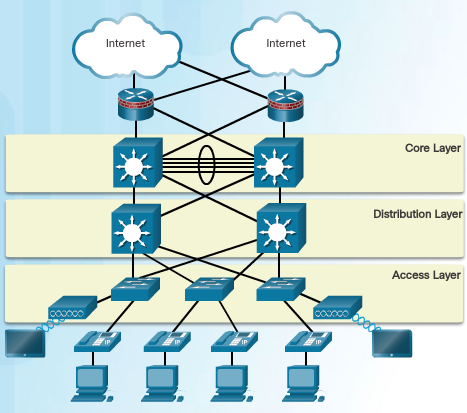
\includegraphics[width=0.7\textwidth]{pictures/Hierarchical-model.png}
\caption{Three-layer hierarchical design model}
\label{Hierarchical-model}
\end{figure}

\begin{figure}[hbtp]
\centering
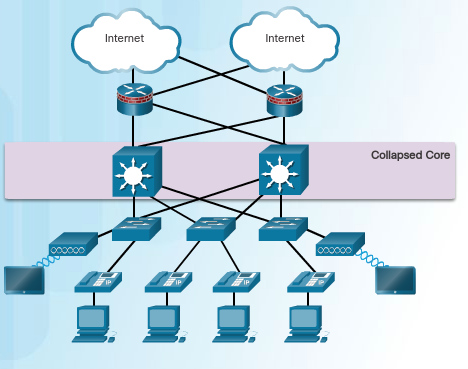
\includegraphics[width=0.7\textwidth]{pictures/collapsed-core.png}
\caption{Collapsed Core}
\label{collapsed-core}
\end{figure}

Even though the hierarchical model has three layers, some smaller enterprise networks may implement a two-tier hierarchical design. In a two-tier hierarchical design, the core and distribution layers are collapsed into one layer, as shown in Figure \ref{collapsed-core}.

\section{Expanding the network}

One method of implementing \textbf{Redundancy} is by installing duplicate equipment and providing failover services for critical devices. Another method of implementing redundancy is redundant paths.\\

A \textbf{failure domain} is the area of a network that is impacted when a critical device or network service experiences problems. The use of redundant links and reliable enterprise-class equipment minimize the chance of disruption in a network. Smaller failure domains reduce the impact of a failure on company productivity.\\

To minimize failure domain, routers or multilayer switches, are usually deployed in pairs, with access layer switches evenly divided between them. This configuration is referred to as a \textbf{switch block}. Each switch block acts independently of the others.

\paragraph{Increasing Bandwidth:} Link aggregation allows an administrator to increase the amount of bandwidth between devices by creating one logical link made up of several physical links. EtherChannel is a form of link aggregation used in switched networks. The EtherChannel is seen as one logical link using an EtherChannel interface. Most configuration tasks are done on the EtherChannel interface, instead of on each individual port, ensuring configuration consistency throughout the links.

\paragraph{Wireless connection:} To communicate wirelessly, end devices require a wireless NIC that incorporates a radio transmitter/receiver and the required software driver to make it operational. Additionally, a wireless router or a wireless access point (AP) is required for users to connect.

\paragraph{Fine-tuning Routing Protocols:} Advanced routing protocols, such as OSPF and EIGRP are used in large networks. Link-state routing protocols such as Open Shortest Path First (OSPF) works well for larger hierarchical networks where fast convergence is important. Another popular routing protocol for larger networks is Enhanced Interior Gateway Routing Protocol (EIGRP). Cisco developed EIGRP as a proprietary distance vector routing protocol with enhanced capabilities.

\section{Selecting network devices}
\subsection{Switch hardwares}
There are five categories of switches for enterprise networks:

\begin{itemize}
\item \textbf{Campus LAN Switches} -- To scale network performance in an enterprise LAN, there are core, distribution, access, and compact switches.
\item \textbf{Cloud-Managed Switches} -- The Cisco \textbf{Meraki} cloud-managed access switches enable virtual stacking of switches. They monitor and configure thousands of switch ports over the web, without the intervention of onsite IT staff.

\item \textbf{Data Center Switches} -- A data center should be built based on switches that promote infrastructure scalability, operational continuity, and transport flexibility. The data center switch platforms include the Cisco Nexus Series switches and the \textbf{Cisco Catalyst 6500 Series} switches.

\item \textbf{Service Provider Switches} -- Service provider switches fall under two categories: aggregation switches and Ethernet access switches. \textbf{Aggregation switches} are carrier-grade Ethernet switches that aggregate traffic at the edge of a network. \textbf{Ethernet access switches} feature application intelligence, unified services, virtualization, integrated security, and simplified management.

\item \textbf{Virtual Networking} -- Cisco \textbf{Nexus} virtual networking switch platforms provide secure multi-tenant services by adding virtualization intelligence technology to the data center network.
\end{itemize}

There are some terminologies that an administrator to be able to choose the right switch platform:
\begin{itemize}
\item \textbf{Port density} is the number of ports available on a single switch.
\item \textbf{Forwarding rates} define the processing capabilities of a switch by rating how much data the switch can process per second.
\item \textbf{Wire speed}  is the data rate that each Ethernet port on the switch is capable of attaining. Data rates can be 100 Mb/s, 1 Gb/s, 10 Gb/s, or 100 Gb/s.
\item \textbf{PoE} (Power over Ethernet) allows the switch to deliver power to a device over the existing Ethernet cabling.  This feature can be used by IP phones and some wireless access points.
\item \textbf{Multilayer switches}, so called Layer-3 switches,  are typically deployed in the core and distribution layers of an organization's switched network
\end{itemize}
\subsubsection{Router hardware}
There are three categories of routers:
\begin{itemize}
\item \textbf{Branch Routers} -- Branch routers optimize branch services on a single platform while delivering an optimal application experience across branch and WAN infrastructures.
\item \textbf{Network Edge Routers} -- Network edge routers enable the network edge to deliver high-performance, highly secure, and reliable services that unite campus, data center, and branch networks.
\item \textbf{Service Provider Routers} -- Service provider routers differentiate the service portfolio and increase revenues by delivering end-to-end scalable solutions and subscriber-aware services.
\end{itemize}

\chapter{WAN concepts}

\section{WAN Technologies overview}

\subsection{Topology}

A WAN operates beyond the geographic scope of a LAN. WANs are used to interconnect the enterprise LAN to remote LANs in branch sites and telecommuter sites. A WAN is owned by a service provider whereas a LAN is typically owned by an organization. An organization must pay a fee to use the WAN service provider’s network services to connect remote sites.\\

\begin{figure}[hbtp]
\centering
\subfigure[Point-to-point]
	{
		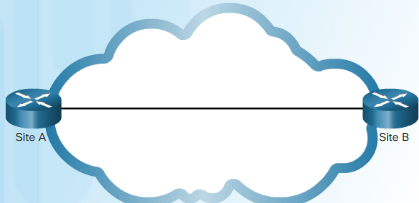
\includegraphics[width=0.4\textwidth]{pictures/WANtopology1.PNG}
		\label{WANtopology1}	
	}
\subfigure[Hub-and-Spoke]
	{
		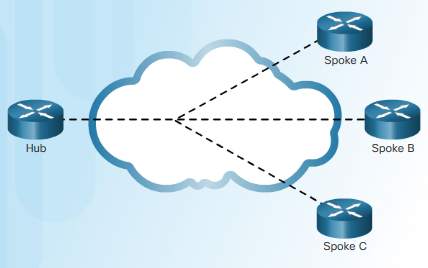
\includegraphics[width=0.4\textwidth]{pictures/WANtopology2.PNG}
		\label{WANtopology2}
	}
\subfigure[Full Mesh]
	{
		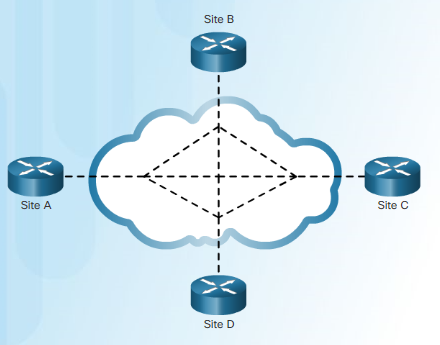
\includegraphics[width=0.4\textwidth]{pictures/WANtopology3.PNG}
		\label{WANtopology3}
	}
\subfigure[Dual-homed]
	{
		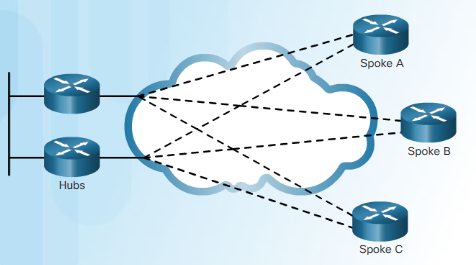
\includegraphics[width=0.4\textwidth]{pictures/WANtopology4.PNG}
		\label{WANtopology4}
	}
\caption{Four common WAN topologies}
\end{figure}

\paragraph{Point-to-Point topology} employs a point-to-point circuit between two endpoints (Figure \ref{WANtopology1}). Typically involves a dedicated leased-line connection such as a T1/E1 line.

\paragraph{Hub-and-Spoke} An example of a single-homed topology. Applicable when a private network connection between multiple sites is required. A single interface to the hub can be shared by all spoke circuits (Figure \ref{WANtopology2}).

\paragraph{Full Mesh} A disadvantage of the hub-and-spoke topology is that all communication has to go through the hub. With a full mesh topology using virtual circuits, any site can communicate directly with any other site (Figure \ref{WANtopology3}). A disadvantage is the large number of virtual circuits that need to be configured and maintained.

\paragraph{Dual-homed Topology} Provides redundancy and load balancing, however more expensive to implement than single-homed topologies(Figure \ref{WANtopology4}). Requires additional networking hardware including routers and switches. More difficult to implement since they require complex configurations.

\subsection{Terminology}

WAN operations focus primarily on the Layer 1 and 2 of the OSI Model. One primary difference between a WAN and a LAN is that a company must subscribe to an outside WAN service provider to use WAN carrier network services.\\

\begin{figure}[hbtp]
\caption{Common WAN terminology}\label{terminology}
\centering
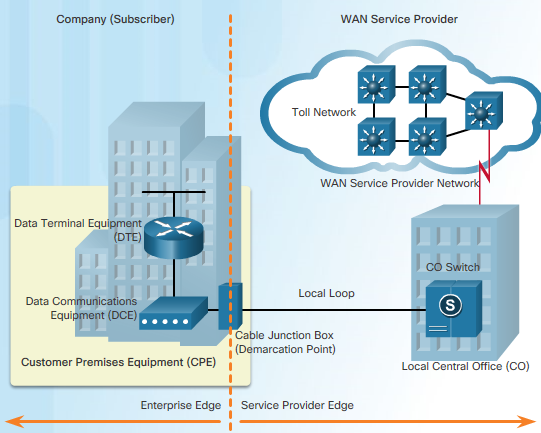
\includegraphics[ width=0.7\textwidth ]{pictures/DCE.PNG}
\end{figure}

Terminology commonly used to describe WAN connections (Figure \ref{terminology}):

\begin{itemize}
\item \textbf{Customer Premises Equipment (CPE)} Consists of devices and inside wiring located on the enterprise edge connecting to a carrier.

\item \textbf{Central Office (CO)} is the local service provider facility that connects the CPE to the provider network.

\item \textbf{Local Loop (last mile)} is the actual copper or fiber cable that connects the CPE to the CO.

\item \textbf{Data Terminal Equipment (DTE)} is usually a router that pass the data from a customer network to DCE.

\item \textbf{Data Communications Equipment (DCE)} is usually a modem that puts data on the local loop by converting digital signals into analog signals. It connects subscribers to the ISP provider.

\item \textbf{Demarcation Point} is a point established in a building to separate customer equipment from service provider equipment. It is the place where the responsibility for the connection changes from the user to the service provider.

\item \textbf{Toll network} consists of the longhaul, all-digital, fiber-optic communications lines and other equipment inside the WAN provider network.
\end{itemize}

\begin{figure}[hbtp]
\caption{WAN devices}\label{Device}
\centering
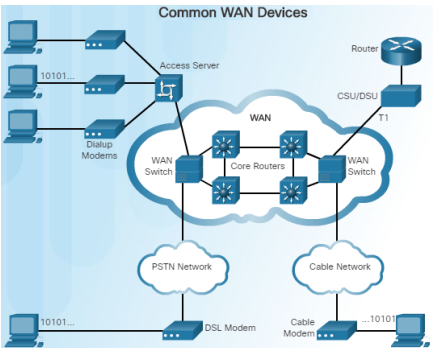
\includegraphics[scale=1]{pictures/Device.PNG}
\end{figure}

There are many types of devices that are specific to WAN environments (Figure \ref{Device}):

\begin{itemize}
\item \textbf{Dialup modem} converts (modulates) the digital signals (produced by a computer) into analog signals (voice frequencies).

\item \textbf{Broadband modem} converts the digital signals into analog signals transferred via high-speed DSL or cable Internet service.

\item \textbf{Access server} controls and coordinates dialup modem, dial-in and dial-out user communications.


\item \textbf{CSU/DSU} is only used for \textbf{Leased line}. The CSU provides termination for the digital signal and ensures connection integrity through error correction and line monitoring. The DSU converts line frames into frames that the LAN can interpret and vice versa.
\end{itemize}

WAN technologies are either circuit-switched or packet-switched:

\paragraph{Circuit Switching} dynamically establishes a \emph{dedicated virtual connection} for voice or data between a sender and a receiver. Communication can't start until the connection is established through the service provider network. The two most common types of circuit-switched WAN technologies are \textbf{PSTN} and \textbf{ISDN}.

\paragraph{Packet Switching} splits traffic data into packets that are routed over a shared network. A circuit does not need to be established and many pairs of nodes can communicate over the same channel. Packet switching costs less than circuit switching, however, latency and jitter are greater in packet-switching networks. There are two approaches to packet-switched network link determination:

\begin{itemize}
\item \textbf{Connectionless systems:} Full addressing information must be carried in each packet. The \textbf{Internet} is an example of a connectionless system. 
\item \textbf{Connection-oriented systems:} The network predetermines the route for a packet, and each packet only has to carry an identifier. An example of a connection-oriented system is \textbf{Frame Relay} (DLCIs are the identifiers).
\end{itemize}

\section{WAN connection}

There are several WAN access connection options (figure \ref{WANaccess}) that ISPs can use to connect the local loop to the enterprise edge.\\

\begin{figure}[hbtp]
\caption{WAN access options}\label{WANaccess}
\centering
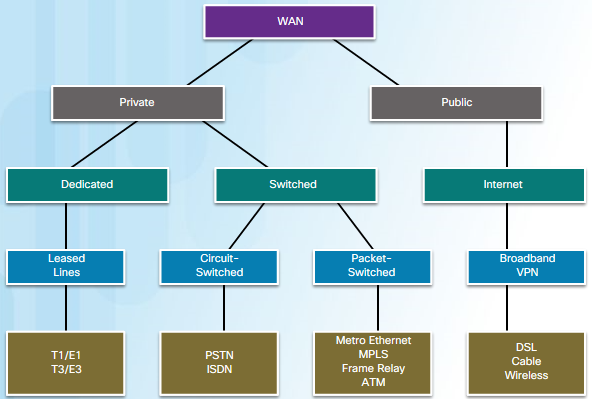
\includegraphics[ width=0.7\textwidth ]{pictures/WANaccess.PNG}
\end{figure}

Service provider networks are complex and consist mostly of high-bandwidth fiber-optic media, using SONET and SDH standard. A newer fiber-optic media development for long-range communications is called dense wavelength division multiplexing (DWDM).

\subsection{Private WAN Infrastructures}

\paragraph{Leased lines} are \emph{permanent dedicated point-to-point} connections from the customer premises to the provider network. The organization pays a monthly lease fee to a service provider to use the line. Leased lines require little installation and maintenance expertise, offer high quality and availability. However, they are expensive and has limited flexibility.

\paragraph{Dialup}transports binary computer data through the voice telephone network using a modem. Dialup access is suitable when intermittent, low-volume data transfers are needed. The advantages of modem and analog lines are simplicity, availability, and low implementation cost. The disadvantages are the low data rates and a relatively long connection time. 

\paragraph{ISDN}is a \emph{circuit-switching} technology that enables the local loop of a PSTN (Public switched telephone network) to carry digital signals. It can provide additional capacity as needed on a leased line connection or can also be used as a backup. ISDN has declined in popularity due to DSL and other broadband services. There are two types of ISDN Interfaces: BRI (2 B-channels, 1 D-channel), PRI (23 B-channel, 1 D-channel)

\paragraph{Frame Relay}is a Layer-2 WAN technology used to interconnect enterprise LANs. Frame Relay creates PVCs (Private Virtual Circuits) to connect multiple sites, and carry voice and data traffic. PVCs are uniquely identified by a DLCI (Data-Link Connection Identifier). The PVCs and DLCIs ensure bidirectional communication between one DTE device to another.

\paragraph{ATM} is built on a \emph{cell-based} architecture rather than on a frame-based architecture. ATM cells are always a \emph{fixed} length of \textbf{53 bytes}. ATM is well-suited for voice and video traffic because this traffic is intolerant of delay.s

\paragraph{Ethernet WAN:}Originally Ethernet was not suitable as a WAN access technology because the maximum cable length was one kilometer. However, \emph{fiber-optic} cables have made Ethernet a reasonable WAN access option. There are several benefits to an Ethernet WAN: Reduced expenses and administration, Easy integration with existing networks, Enhanced business productivity. Ethernet WANs have replaced Frame Relay and ATM.

\paragraph{MPLS} is a \emph{multiprotocol} high-performance WAN technology that directs data from one router to the next. MPLS is based on \emph{short path labels} rather than IP network addresses.  It uses labels which tell a router what to do with a packet. The labels identify paths between distant routers rather than endpoints, and while MPLS actually routes IPv4 and IPv6 packets, everything else is switched. Furthermore, MPLS can deliver any type of packet between sites and encapsulate them of various network protocols.

\paragraph{VSAT} is a solution that creates a private WAN using \emph{satellite} communications in remote locations where there are no service providers that offer WAN service.

\subsection{Public WAN Infrastructures}

\paragraph{DSL}is an always-on connection technology that uses existing \emph{twisted-pair telephone} lines to transport high-bandwidth data. A DSL modem converts an Ethernet signal from the user device to a DSL signal. Key components in the DSL connection: \emph{DSL modem (subscriber end)} and \emph{DSLAM (ISP end)}. The advantage that DSL has over cable technology is that DSL is not a shared medium -- each user has a separate direct connection to the DSLAM.

\paragraph{Cable} is widely used in urban areas to distribute television signals. Network access is available from television providers. This allows for greater bandwidth than the conventional telephone local loop. Two types of equipment are required: \emph{Cable Modem (subscriber end)} and \emph{CMTS (ISP end)}.

\paragraph{WiMAX} is a new technology that operates in a similar way to Wi-Fi, but at higher speeds, over greater distances, and for a greater number of users. It uses a network of WiMAX towers that are similar to cell phone towers. 

\paragraph{Satellite Internet}Typically used by rural users where cable and DSL are not available. Cable and DSL have higher download speeds, but satellite systems are about 10 times faster than an analog modem. 

\paragraph{VPN}is an encrypted connection between private networks over Internet. VPN uses virtual connections called VPN tunnels, which are routed through the Internet from the private network of the company to the remote site or employee host. There are several benefits to using VPN: cost savings, security, scalability, compatibility with broadband technology. There are two types of VPN access: 

\begin{itemize}
\item \textbf{Site-to-site VPN:} connect entire networks to each other, for example, connecting a branch
office network to a company headquarters network. 
\item \textbf{Remote-access VPN:} enable individual hosts, such as  extranet consumers, to access a company network securely over the Internet.
\end{itemize}

\paragraph{Dynamic Multipoint VPN (DMVPN)} is a Cisco software solution for building multiple VPNs. DMVPN is built on three protocols: NHRP, IPsec, and mGRE. NHRP is the distributed address \emph{mapping} protocol for VPN tunnels. IPsec \emph{encrypts} communications on VPN tunnels. The mGRE protocol allows the dynamic creation of \emph{multiple spoke tunnels} from one permanent VPN \emph{hub}.
\chapter{Network evolution}

\section{IoT}

\subsection{IoT pillars}



\part{SWITCHING TECHNOLOGIES}
\chapter{Switch}

\section{Operation}

\subsection{Switch boot sequence}

After a Cisco switch is powered on, it goes through the following boot sequence:

\begin{enumerate}
\item The switch loads a power-on self-test (POST) program stored in ROM.

\item Boot loader software is loaded.

\item The boot loader initializes the CPU registers.

\item The boot loader initializes the flash file system.

\item The boot loader loads IOS image into RAM and gives control of the switch to the IOS.

\item The IOS initializes the startup-config file, which is stored in NVRAM.
\end{enumerate}

The boot loader software finds the Cisco IOS image using \emph{Boot environment variables}. If this variable is not set, the switch attempts to load and execute the first executable file it finds. It does a recursive search until finally searching the root directory. For this reason, on a Cisco 2960 switch, the IOS image file is normally contained in a directory that has the same
name root name as the image file.\\

The Boot environment variable is set using the \verb|boot system| command:

\begin{verbatim}
S1(config)# boot system flash:/c2960-lanbasek9-mz.150-2.SE/c2960-lanbasek9-
mz.150-2.SE.bin
\end{verbatim}

Use the command \verb|show boot| to see content of the Boot environment variable and what the current IOS boot file is set to.

\subsection{MAC address table}

A Layer 2 Ethernet switch uses MAC addresses to make forwarding decisions. It consults a MAC address table to make a forwarding decision for each frame. By default, most Ethernet switches keep an entry in the MAC address table for 5 minutes.

\paragraph{Learning MAC Address} The switch dynamically builds the MAC address table by examining the source MAC address of the frames received on a port. Every frame that enters a switch is checked for new information to learn. If the source MAC address does not exist, it is added to the table along with the incoming port number. If the source MAC address does exist, the switch updates the refresh timer for that entry.  If the source MAC address does exist in the table but on a different port, the switch treats this as a new entry.

\paragraph{Forwarding MAC Address} Next, if the destination MAC address is a unicast address, the switch will look for a match between the destination MAC address of the frame and an entry in its MAC address table. If the destination MAC address is in the table, it will forward the frame out the specified port. If the destination MAC address is not in the table, the switch will forward the frame out all ports except the incoming port. If the destination MAC address is a broadcast or a multicast, the frame is also flooded out all ports except the incoming port.\\

A switch can have multiple MAC addresses associated with a single port. This is common when the switch is connected to another switch.

\subsection{Frame forwarding method}

A switch makes a decision on frame forwarding based on two criteria: \textbf{Ingress port} and \textbf{Destination address}. Switches use one of the following forwarding methods:  Store-and-forward switching and Cut-through switching.

\paragraph{Store-and-forward switching} has two primary characteristics that distinguish it from cut-through: \textbf{error checking} and \textbf{automatic buffering}. When the switch receives the frame, it stores the data in buffers until the complete frame has been received. In this process, the switch also performs an error checking using the CRC trailer portion of the Ethernet frame. When an error is detected in a frame, the switch discards the frame. Discarding frames with errors reduces the amount of bandwidth consumed by corrupt data. Store-and-forward switching is required for Quality of Service (QoS).

\paragraph{Cut-through switching}  There are two primary characteristics of cut-through switching: \textbf{rapid frame forwarding} and \textbf{fragment free}. The switch buffers just enough of the frame to read the destination MAC address (first 6 bytes) so that it can determine to which port to forward the data. No error detection is performed. There are two variants of cut-through switching: 

\begin{itemize}
\item \textbf{Fast-forward switching:} the switch immediately forwards a packet after reading the destination address. It offers the lowest level of latency. 

\item \textbf{Fragment-free switching} the switch waits for the collision window (64 bytes) to pass before forwarding the frame. The reason is that most network errors and collisions occur during the first 64 bytes. 
\end{itemize}

\subsection{Switching domain}

\paragraph{Collision domain:} In \emph{hub-based} Ethernet segments, network devices must take turns when transmitting. The network segments that share the same bandwidth between devices are known as collision domains. Therefore, all ports of a hub are in the same collision domain. However, each port on a switch, or a router is a separate collision domain.

\begin{figure}[hbtp]
\caption{An example of collision domains}
\centering
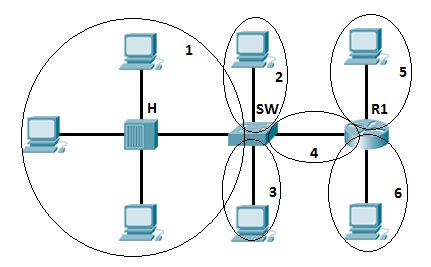
\includegraphics[scale=0.8]{pictures/CollisionDomains.jpg}
\end{figure}

\paragraph{Broadcast domain}is a domain in which a broadcast is forwarded. A broadcast domain contains all devices that can reach each other at the data link layer (OSI layer 2) by using broadcast. All ports on a hub or a switch are by default in the same broadcast domain. All hosts in the a VLAN are in the same broadcast domain regardless connecting to different switches. Every port on a router locates in a separate broadcast domain. Note that routers don't forward broadcasts from one broadcast domain to another.


\subsection{Memory Buffering on Switches}

There are two methods of memory buffering: Port-based Memory Buffering and Shared Memory Buffering.

\paragraph{Port-based Memory Buffering} Frames are stored in queues that are linked to specific incoming and outgoing ports. A frame is transmitted to the outgoing port only when all the frames ahead of it in the queue have been successfully transmitted. 

\paragraph{Shared Memory Buffering} deposits all frames into a common memory buffer that all the ports on the switch share.  The frames in the buffer are linked dynamically to the destination port. This allows the packet to be transmitted on a port without order and waiting. This method permits larger frames to be transmitted with fewer dropped frames. 

\section{Recovering from system crash}

The boot loader command line supports commands to format the flash file system, reinstall the operating system software, recover from system crash, recover a forgotten password. The boot loader command line can be accessed through a console connection following these steps:

\begin{enumerate}
\item Connect a PC by console cable to the switch console port. Configure terminal emulation software to connect to the switch.

\item Power off the switch by unplugging the switch power cord.

\item Reconnect the power cord to the switch and, within 15 seconds, press and hold down the Mode button while the System LED until it turns briefly amber and then solid green.
\end{enumerate}

\section{Configuration}

\subsection{Basic switch management}

To prepare a switch for remote management, it must be configured with an SVI, IP address, a subnet mask, and a default gateway. This is similar to configuring the IP address information on host devices.\\

\begin{verbatim}
S1(config)# interface vlan 99
S1(config-if)# ip address 172.17.99.11 255.255.255.0
S1(config-if)# no shutdown
S1(config-if)# exit
S1(config)#
S1(config)# ip default-gateway 172.17.99.1
S1(config)# end
\end{verbatim}

\note These IP settings are only for remote management access to the switch. The IP settings do not allow the switch to route Layer 3 packets.

\subsection{Duplex configuration}

When a switch port is operating in full-duplex mode, there is no collision domain associated with the port. In contrast, half-duplex creates collision domain.\\

The following command manually sets the F0/1 to full duplex and 100 Mb/s.

\begin{verbatim}
S1(config)# interface fa 0/1
S1(config-if)# duplex full
S1(config-if)# speed 100
S1(config-if)# end
\end{verbatim}

The \verb|show interface| command can be used to verify if the interface accepted the settings.

\subsection{Auto-MDIX}

When auto-MDIX is enabled, the interface automatically detects the required cable connection type (straight-through or crossover) and configures the connection appropriately. In other words, with auto-MDIX enabled, either type of cable can be used to connect to other devices.

\begin{verbatim}
S1(config)# interface fastethernet 0/2
S1(config-if)# mdix auto
S1(config-if)# end
\end{verbatim}

To examine the auto-MDIX setting for a specific interface, use the \verb|show controllers| \verb|ethernet-controller| command with the \verb|phy| keyword. The \verb|phy| keyword displays the status of the internal registers on the switch physical layer device (PHY) and includes the operational state of the auto-MDIX feature on an interface. 

\begin{verbatim}
S1# show controllers ethernet-controller fa 0/2 phy | include Auto-MDIX
Auto-MDIX : On [AdminState=1 Flags=0x00056248]
S1#
\end{verbatim}


\subsection{SSH}

Before configuring SSH, the switch must be minimally configured with a unique hostname and the correct network connectivity settings. To configure SSH on a switch, following these steps:

\begin{verbatim}
S1(config)# ip domain-name cisco.com
S1(config)# ip ssh version 2
S1(config)# crypto key generate rsa
The name for the keys will be: S1.cisco.com
...
How many bits in the modulus [512]: 1024
...
S1(config)#
S1(config)# username admin secret ccna
S1(config)#
S1(config)# line vty 0 15
S1(config-line)# transport input ssh
S1(config-line)# login local
S1(config-line)# end
\end{verbatim}

To display the version and configuration data for SSH on the device that you configured as an SSH server, use the \verb|show ip ssh| command. To check the SSH connections
to the device, use the \verb|show ssh| command.

\subsection{Port security}

One way to secure ports is by implementing a feature called \emph{port security}. Port-security limits the number of valid MAC addresses allowed on a port.
The MAC addresses of legitimate devices are allowed access, whereas other MAC addresses are denied. If a port is configured as a secure port and the maximum number of MAC addresses is reached, any additional attempts to connect by unknown MAC addresses generate a security violation.\\

Enable port-security feature will not work until the following command is executed:

\begin{verbatim}
S1(config)# interface fastethernet 0/19
S1(config-if)# switchport port-security
\end{verbatim}

The type of secure address is based on the configuration and includes the following:

\begin{itemize}
\item \textbf{Static secure MAC addresses} are manually configured on a port by using the below command. They are stored in the address table and are added to the running configuration on the switch.

\begin{verbatim}
S1(config)# interface f0/1
S1(config-if)# switchport port-security mac-address aaaa.cafe.bbbb
\end{verbatim}

\item \textbf{Dynamic secure MAC addresses} are dynamically learned and stored only in the address table. They are removed when the switch restarts.

\item \textbf{Sticky secure MAC addresses} can be dynamically learned or manually configured, and then stored in the address table and added to the running configuration. When the following command is entered, the switch converts all dynamically learned MAC addresses, including those that were dynamically learned before sticky learning was enabled, into sticky secure MAC addresses. If sticky learning is disabled, the sticky secure MAC addresses remain part of the address table but are removed from the running configuration.

\begin{verbatim}
S1(config)# interface f0/1
S1(config-if)# switchport port-security mac-address sticky
\end{verbatim}
\end{itemize}

An interface can be configured for one of three violation modes: Protected, Restricted, and Shutdown. In these modes, a switch drops all frames with unknown source addresses until a sufficient number of these MAC addresses are removed, or the number of maximum allowable addresses is increased. No error messages are displayed in these modes.\\

\begin{table}[hbtp]
\centering\caption{Security violation mode}
\begin{tabular}{ | p{3cm} | p{3cm} | p{3cm} | p{3cm} | }

\hline
\head{Violation mode} & \head{Syslog message} & \head{Increase violation counter} & \head{Shut down port}\\
\hline

Protected & & & \\ \hline
Restricted & * & * & \\ \hline
Shutdown & & * & *\\ \hline

\end{tabular}
\end{table}

To change the violation mode on a switch port, use the following command:

\begin{verbatim}
S1(config)# interface f0/1
S1(config-if)# switchport port-security violation protect
S1(config-if)# switchport port-security violation restrict
S1(config-if)# switchport port-security violation shutdown
\end{verbatim}

\textbf{Shutdown} is the default violation mode. A port-security violation in this mode causes the interface to become \emph{error-disabled}. You can bring an error-disabled interface back to normal by entering \verb|shutdown| followed by \verb|no shutdown| command.\\

When a port is error-disabled, the port LED will turn off. The \verb|show interface| command identifies the port status as \verb|err-disabled|. The output of the \verb|show port-security interface| command shows the port status as \verb|secure-shutdown|.\\

\textbf{Restrict} is the only port security mode that can assist with troubleshooting by sending syslog messages and keeping count of violations.

\section{Troubleshooting}

\subsection{Gathering symptoms}

The output from the \verb|show interfaces| command can be used to detect common media issues.

\begin{verbatim}
S1# show interfaces FastEthernet 0/1
FastEthernet0/1 is up, line protocol is up (connected)
Hardware is Lance, address is 0022.91c4.0e01 (bia 0022.91c4.0e01)
MTU 1500 bytes, BW 100000 Kbit/sec, DLY 100 usec,
<output omitted>
\end{verbatim}

The first parameter (\verb|FastEthernet0/1 is up|) refers to the \emph{physical layer} and indicates whether the interface is receiving a carrier detect signal. The second parameter (\verb|line protocol is up|) refers to the \emph{data link layer} and indicates whether the data link layer protocol keepalives are being received.\\

If the interface is up and the line protocol is down, there could be an \emph{encapsulation} type mismatch, or the interface on the other end could be \emph{error-disabled}.\\

If the line protocol and the interface are both down, a cable is not attached, or the other end of the connection may be administratively down.\\

If the interface is administratively down, it has been manually disabled (the \verb|shutdown| command has been issued) in the active configuration.\\

\begin{verbatim}
S1# show interfaces FastEthernet 0/1
FastEthernet0/1 is up, line protocol is up (connected)
<output omitted>

3 input errors, 3 CRC, 0 frame, 0 overrun, 0 ignored
0 watchdog, 120 multicast, 0 pause input
0 input packets with dribble condition detected
3594664 packets output, 436549843 bytes, 0 underruns
<output omitted>
\end{verbatim}

\textbf{Input errors} is the sum of all errors in frames that were received on the interface being examined. The reported input errors from the above output of \verb|show interfaces| command include the following:

\begin{itemize}
\item \textbf{Runt frames:} Ethernet frames that are shorter than the 64-byte (minimum allowed length of a frame) are called runt frames. Runt frames are caused by malfunctioning NIC or collisions.

\item \textbf{Giant:} Ethernet frames that are larger than 1518-byte (maximum allowed size of a frame) are called giants.

\item \textbf{CRC errors:} Common causes come from the cable (electrical interference, loose or damaged connections, and incorrect cabling). If you see many CRC errors, there is too much noise on the cable and you should inspect the cable. You should also search for and eliminate noise sources.
\end{itemize}

\begin{verbatim}
S1# show interfaces FastEthernet 0/1
FastEthernet0/1 is up, line protocol is up (connected)
<output omitted>

8 output errors, 1790 collisions, 10 interface resets
0 unknown protocol drops
0 babbles, 235 late collision, 0 deferred
0 lost carrier, 0 no carrier, 0 pause output
0 output buffer failures, 0 output buffers swapped out
\end{verbatim}

\textbf{Output errors} is the sum of all errors that prevented the final transmission of frames out the interface that is being examined. The reported output errors from the above output of \verb|show interfaces| command include the following:

\begin{itemize}
\item \textbf{Collisions:} Collisions in half-duplex operations are normal. However, you should never see collisions on an interface configured for full-duplex communication.

\item \textbf{Late collision:} A late collision refers to a collision that occurs after \textbf{512 bits} of the frame have been transmitted. Common causes: Excessive cable lengths, Duplex mismatch.
\end{itemize}

\subsection{Take action}

If the interface is down, take these two actions:

\begin{enumerate}
\item Check the \emph{cable}. Make sure the proper and non-damaged cables are being used.

\item If the interface is still down, the problem may be due to a \emph{speed mismatch}. Manually set the same speed on both connection ends if this problem is suspected.
\end{enumerate}

If the interface is up, but issues with connectivity are still present, do the following:

\begin{enumerate}
\item Using the \verb|show interfaces| command, check for indications of excessive \emph{noise}. Indications may include an increase in the counters for runts, giants, and CRC errors. If there is excessive noise, find and remove the source of the noise, verify that the cable does not exceed the maximum cable length and check the cable type.

\item If noise is not an issue, check for excessive \emph{collisions}. If there are collisions or late collisions, the problem may be due to \emph{duplex mismatch}. If this is true, manually set the duplex to full on both ends of the connection.
\end{enumerate}
\chapter{VLAN}

\section{Overview}

VLANs provide a way to group devices within a LAN. Devices within a VLAN act as if they are in their own independent network, even if they share a common infrastructure with other VLANs. The transmission of unicast, multicast, and broadcast traffic from a host in a particular VLAN are restricted to the devices that are in that VLAN.\\

The primary benefits of using VLANs are as follows:

\begin{itemize}
\item \textbf{Security:} Groups that have sensitive data are separated from the rest of the network, decreasing the chances of confidential information breaches. 

\item \textbf{Better performance:} Dividing flat Layer 2 networks into multiple logical workgroups (broadcast domains) reduces unnecessary traffic on the network and
boosts performance.

\item \textbf{Grouping:} VLANs allows logical grouping of users by function. 
\end{itemize}

There are a number of distinct types of VLANs: 

\begin{itemize}
\item \textbf{Default VLAN:} By default, all switch ports are assigned to default VLAN (VLAN 1). VLAN 1 has all the features of any VLAN, except it cannot be renamed or deleted.

\item \textbf{Native VLAN} is assigned to trunk ports. It serves as a common identifier on opposite ends of a trunk link. It is a best practice to configure a native VLAN for all trunk ports in the switched domain.

\item \textbf{Data VLAN} is configured to carry user-generated traffic. A VLAN carrying voice or management traffic would not be a data VLAN. 

\item \textbf{Management VLAN} is configured to access the management capabilities of a switch. To create the management VLAN, the SVI\footnote{Switch Virtual Interface} of that VLAN is assigned an IP address and a subnet mask. VLAN 1 would be a bad choice for the management VLAN.

\item \textbf{Voive VLAN} is a separate VLAN needed to support Voice over IP (VoIP). 
\end{itemize}

\textbf{Normal range} VLANs are identified by a VLAN ID between 1 and 1005. Configurations are stored within a VLAN database file, called \verb|vlan.dat|. This file is located in the flash memory of the switch. VTP can only learn and store normal range VLANs.\\

\textbf{Extended Range} VLANs are identified by a VLAN ID between 1006 and 4094. Configurations are not written to the \verb|vlan.dat| file, but instead, stored in running configuration file. VTP does not learn extended range VLANs.

\section{VLAN tag}

\subsection{What is tagging?}

A \textbf{trunk} is a point-to-point link between two network devices that carries more than one VLAN. VLAN trunks allow all VLAN traffic to propagate between switches so that devices that are in the same VLAN, but connected to different switches.\\

When Ethernet frames are placed on a trunk, information about the VLANs to which they belong must be added. This process, called \textbf{tagging}, is accomplished by using the IEEE \textbf{802.1Q} header.\\

\begin{figure}[hbtp]
\caption{Fields in Ethernet 801.Q frame}\label{tagging}
\centering
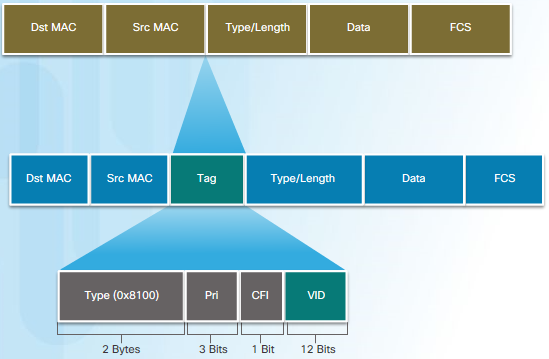
\includegraphics[ width=0.6\textwidth ]{pictures/tagging.PNG}
\end{figure}


The 802.1Q header includes a 4-byte tag inserted within the original Ethernet frame header (Figure \ref{tagging}), specifying the VLAN to which the frame belongs. When the switch receives a frame on an \emph{access} port assigned to a VLAN, the switch inserts a VLAN tag in the frame header, recalculates the FCS\footnote{Frame Check Sequence}, and sends the tagged frame out of a trunk port.\\

\subsection{VLAN tag field}

The VLAN tag field (Figure \ref{tagging}) consists of: 

\begin{itemize}
\item \textbf{Type:} A 2-byte value called the tag protocol ID (TPID) value. For Ethernet, it is set to hexadecimal 0x8100.

\item \textbf{User priority:} A 3-bit value that supports level or service implementation

\item \textbf{Canonical Format Identifier (CFI):} A 1-bit identifier that enables Token Ring frames to be carried across Ethernet links.

\item \textbf{VLAN ID:} A 12-bit VLAN identification number that supports up to 4096 VLAN IDs.
\end{itemize}

After the switch inserts the Type and tag control information fields, it recalculates the FCS values and inserts the new FCS into the frame.

\subsection{Native VLAN and tagging}

A trunk port always forwards untagged frames to the native VLAN. If there are no devices associated with the native VLAN and there are no other trunk ports, then the frame is dropped. Additionally, if an 802.1Q trunk port receives a tagged frame with the VLAN ID that is the same as the native VLAN, it drops the frame.

\subsection{Voice VLAN tagging}

The link between the switch and the IP phone acts as a trunk to carry both voice VLAN traffic and data VLAN traffic. The Cisco IP Phone contains an integrated three-port 10/100 switch. The ports provide dedicated connections to these devices:

\begin{itemize}
\item Port 1 connects to the switch or other VoIP device.
\item Port 2 is an internal 10/100 interface that carries the IP phone traffic.
\item Port 3 (access port) connects to a PC or other device.
\end{itemize}

\begin{figure}[hbtp]
\caption{IP phone ports}\label{PhonePort}
\centering
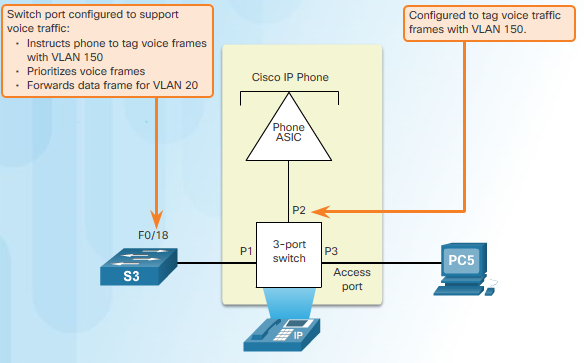
\includegraphics[ width=0.6\textwidth ]{pictures/PhonePort.PNG}
\end{figure}


On the switch, the access is configured to send CDP packets that instruct an attached IP phone to send voice traffic to the switch in one of three ways:

\begin{itemize}
\item In a voice VLAN tagged with a Layer 2 CoS\footnote{Class of Service} priority value
\item In an access VLAN tagged with a Layer 2 CoS priority value
\item In an access VLAN, untagged (no Layer 2 CoS priority value)
\end{itemize}

\section{Configuration}

\subsection{Create VLAN}

A VLAN is created using the \verb|vlan vlan_id| global configuration command. This creates the VLAN and enters VLAN configuration mode. The VLAN can now be assigned a unique name using the \verb|name vlan_name| command.

\begin{verbatim}
S1(config)# vlan 20
S1(config)# name Student
\end{verbatim}

Instead of creating one VLAN at a time, several VLANs can be created using one command. A series of VLAN IDs can be entered separated by commas, or a range of VLAN IDs can be entered separated by hyphens (-). 

\begin{verbatim}
S1(config)# vlan 100,102,105-107
\end{verbatim}

\subsection{Access port}

After creating a VLAN, the next step is to assign access ports to the VLAN. First of all, the port must be assigned as an
access port using the \verb|sw mode access| interface configuration command. Next, assign the port to a VLAN using the \verb|sw access vlan vlan_id| interface configuration command. Note that an access port can belong to only one VLAN at a time.

\begin{verbatim}
S1(config)# interface FastEthernet0/1
S1(config-if)# sw mode access
S1(config-if)# sw access vlan 20
S1(config-if)# end
\end{verbatim}

\subsection{Delete VLAN}

We can delete a VLAN with \verb|no vlan vlan_id| in global configuration mode. However, be careful when removing a VLAN. Before deleting a VLAN, reassign all member ports to a different VLAN. Any ports that are not moved to an active VLAN are unable to communicate with other hosts after the VLAN is deleted. \\

The entire VLAN configuration can be erased using \verb|delete vlan.dat|. This command, along with \verb|erase startup| effectively places the switch into its factory default condition.

\subsection{Trunk port}

To configure a switch port on one end of a trunk link, use the \verb|sw mode trunk| interface configuration command. The native VLAN can also be changed (other than VLAN 1) using \verb|sw trunk native vlan vlan_id|. Always configure both ends of a trunk link with the same native VLAN. \\

Use \verb|sw trunk allowed vlan vlan-list| command to specify the list of VLANs to be allowed on the trunk link.\\

\begin{verbatim}
S1(config)# interface f0/1
S1(config-if)# sw mode trunk
S1(config-if)# sw trunk native vlan 99
S1(config-if)# sw trunk allowed vlan 10,20,30,99
S1(config-if)# end
\end{verbatim}

This configuration assumes the switches automatically use 802.1Q encapsulation on trunk links. Some switches may require manual configuration of the encapsulation. We have to configure 802.1Q encapsulation before trunking mode. Otherwise, the following message will appear:

\begin{verbatim}
Command rejected: An interface whose trunk encapsulation is "Auto" can not be configured to "trunk" mode. 
\end{verbatim}

Whenever this error message appears, use the following solution:

\begin{verbatim}
S1(config)# interface f0/1
S1(config-if)# sw trunk encapsulation dot1q 
S1(config-if)# sw mode trunk
\end{verbatim}

To reset a trunk to allow all VLANs, use the \verb|no sw trunk allowed vlan| interface configuration command. To reset the native VLAN to VLAN 1, use the \verb|no sw trunk native vlan| interface configuration command. To set the port to a non-trunking port, use the \verb|sw mode access| interface command.\\

\subsection{Voice VLAN}

Consider the topology in Figure \ref{VoiceVLAN}. In this example, PC5 is connected to the Cisco IP phone, which in turn is connected to the F0/18 interface on S3. To implement this configuration, Data VLAN 20 (for PC) and Voice VLAN 150 (for IP phone) are created. 

\begin{verbatim}
S3(config)# vlan 20
S3(config-vlan)# name Student
S3(config-vlan)# vlan 150
S3(config-vlan)# name Voice
S3(config-vlan)# exit
S3(config)# 
S3(config)# interface f0/18
S3(config-if)# sw mode access
S3(config-if)# sw access vlan 20
S3(config-if)# 
S3(config-if)# mls qos trust cos
S3(config-if)# sw voice vlan 150
S3(config-if)# end
\end{verbatim}

\begin{figure}[hbtp]
\caption{Sample topology with IP phone}\label{VoiceVLAN}
\centering
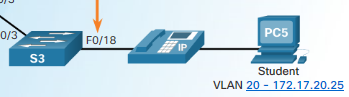
\includegraphics[scale=0.6]{pictures/VoiceVLAN.PNG}
\end{figure}

The command \verb|mls qos trust cos| enables QoS classification based on the class of service (CoS) assigned by the IP phone. The command \verb|sw voice vlan 150| assigns  voice VLAN 150 to port F0/18. 

\subsection{Verification}

VLAN configurations can be validated using the following command:

\begin{verbatim}
S1# show vlan [brief | id vlan-id | name vlan-name | summary]

S1# show vlan name student
S1# show vlan summary
S1# show vlan brief
S1# show interfaces vlan 20
\end{verbatim}

The trunking configuration is verified by the following commands:

\begin{itemize}
\item \verb|show interfaces switchport|
\item \verb|show interface <int> switchport|
\item \verb|show interfaces trunk| 
\end{itemize}

\subsection{Troubleshoot}

\paragraph{IP address} Each VLAN must correspond to a unique IP subnet. If two devices in the same VLAN have different subnet addresses, they cannot communicate. This is a common problem, and it is easy to solve by identifying the incorrect configuration and changing the subnet address to the correct one.

\paragraph{Missing VLAN} Verify whether the port is in the correct VLAN using \verb|show vlan| and \verb|show mac address-table int <int>|. Verify if the VLAN is present in the VLAN database using \verb|show vlan|. Use the \verb|show interfaces switchport| command to verify if the inactive VLAN is assigned to the port.


\paragraph{Native VLAN mismatches} Trunk ports are configured with different native VLANs. This configuration error generates console notifications and can cause inter-VLAN routing issues. To solve the native VLAN mismatch, configure the native VLAN to be the same VLAN on both sides of the link.

\paragraph{Trunk mode mismatches} One trunk port is configured in a mode that is not compatible for trunking on the corresponding peer port. This configuration error causes the trunk link to stop working. Be sure both sides of the trunk are configured with the \verb|sw mode trunk| command. 

\paragraph{Allowed VLANs} The list of allowed VLANs on a trunk has not been updated with the current VLAN trunking requirements. 

\section{Inter-VLAN Routing}

Layer 2 switches have limited IPv4 and IPv6 functionality and cannot perform the routing between VLANs. Any device that supports Layer 3 routing, such as a router or a Layer 3 switch (multiplayer), can be used to perform VLAN routing. Regardless of the device used, the process of forwarding network traffic from one VLAN to another is known as inter-VLAN routing. There are three options for inter-VLAN routing: Legacy inter-VLAN routing, Router-on-a-stick, Layer 3 switching using SVIs.

\subsection{Legacy inter-VLAN routing}

In this legacy approach, inter-VLAN routing is performed by connecting different physical router interfaces to different physical switch ports. The switch ports connected to the router are placed in access mode, and each physical interface is assigned to a different VLAN.

\subsection{Router-on-a-stick}

Router-on-a-stick uses a single physical interface to route traffic between multiple VLANs. The router interface is configured to operate as a trunk link and is connected to a switch port that is configured in trunk mode. \\

Router-on-a-stick performs inter-VLAN routing by accepting VLAN-tagged traffic coming from the switch, and then, \emph{internally} routing between the VLANs using subinterfaces. Subinterfaces are virtual interfaces, associated with a single physical interface. Each subinterface is independently configured with an IP address and VLAN assignment (Figure \ref{InterVLAN}). The IPv4 address of the subinterface acts as the default gateway for all hosts in the corresponding VLAN.\\

\begin{figure}[hbtp]
\caption{Router-on-a-stick topology}\label{InterVLAN}
\centering
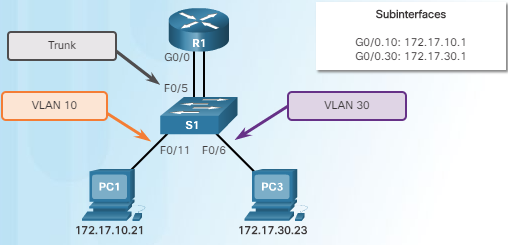
\includegraphics[scale=1]{pictures/InterVLAN.PNG}
\end{figure}


To enable Router-on-a stick, start by enabling trunking on the switch port that is connected to the router.

\begin{verbatim}
S1(config-vlan)# interface f0/5
S1(config-if)# switchport mode trunk
S1(config-if)# end
\end{verbatim}

As for the router, create a subinterface for each VLAN. Then configure 802.1Q trunk for a specific VLAN using \verb|encapsulation dot1q vlan_id|. Next, assign the IPv4 address corresponding to the VLAN subnet. Finally, the physical interface must be enabled. 

\begin{verbatim}
R1(config)# interface g0/0.10
R1(config-subif)# encapsulation dot1q 10
R1(config-subif)# ip address 172.17.10.1 255.255.255.0
R1(config-subif)# 
R1(config-subif)# interface g0/0.30
R1(config-subif)# encapsulation dot1q 30
R1(config-subif)# ip address 172.17.30.1 255.255.255.0
R1(config-subif)# exit
R1(config)# 
R1(config)# interface g0/0
R1(config-if)# no shutdown
\end{verbatim}

\note Use the command \verb|encapsulation dot1q vlan_id native| for the native VLAN. If the \verb|native| keyword option is excluded, the router would consider VLAN 1 as the native VLAN.\\

On the router, use \verb|show vlan| and \verb|show ip route| to verify inter-vlan configuration.

\subsection{Layer 3 switching using SVIs}

Most modern enterprise networks use multilayer switches to achieve much higher packet-switching throughputs (millions of packets per second). Layer 3 switching is much faster than router-on-a-stick, because everything is hardware switched and routed. Despite its price, multilayer switch provide lower latency, support EtherChannel to get more bandwidth. Furthermore, with the multiplayer switch, the network architecture (Figure \ref{NetArch}) is not dependent on STP\footnote{Spanning Tree Protocol, see also section \ref{sec:STP} } anymore because layer 2 loops never occurs in the topology.

\begin{figure}[hbtp]
\caption{Network architecture with multiplayer switches}\label{NetArch}
\centering
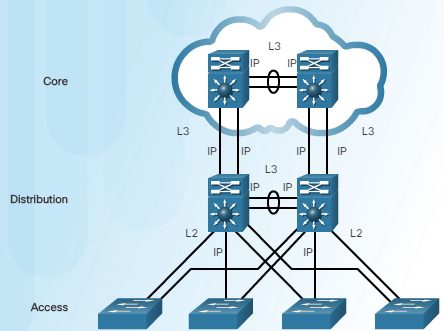
\includegraphics[scale=0.6]{pictures/NetArch.PNG}
\end{figure}


\begin{figure}[hbtp]
\caption{Router-on-a-stick and Multiplayer switch}\label{Layer3sw}
\centering
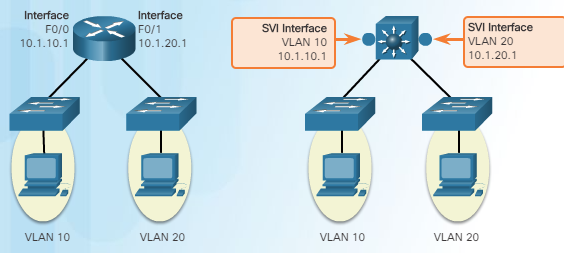
\includegraphics[scale=0.6]{pictures/Layer3sw.PNG}
\end{figure}


Inter-VLAN routing is performed using SVIs and routed ports.
\begin{itemize}
\item \textbf{Routed port:} A pure Layer 3 interface similar to a physical interface on a router. A routed port is not associated with any VLAN. Routed ports are normally implemented between the distribution and the core layer (usually between multiplayer switch and a router or a security device). To configure routed ports, use the \verb|no switchport| interface configuration mode command.

\item \textbf{SVI:} An SVI is configured for each VLAN that exists on the switch. It can perform the same functions as subinterface in Router-on-a-stick method (Figure \ref{Layer3sw}). 
\end{itemize}

\begin{figure}[hbtp]
\caption{Sample topology}\label{Layer3topology}
\centering
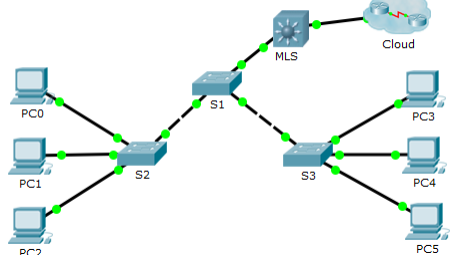
\includegraphics[scale=0.6]{pictures/Layer3topology.PNG}
\end{figure}

Take the multiplayer switch MLS in Figure \ref{Layer3topology} as an example. The first thing to do is enabling layer 3 routing:

\begin{verbatim}
MLS(config)# ip routing
\end{verbatim}

Next, configure G0/2 (connect to the Cloud) as a routed port and assign an IP address:

\begin{verbatim}
MLS(config)# interface g0/2
MLS(config-if)# no switchport
MLS(config-if)# ip address 209.165.200.225 255.255.255.252
\end{verbatim}

Create VLAN 10 and 20, then configure SVI for each of them:

\begin{verbatim}
MLS(config)# vlan 10
MLS(config-vlan)# name Staff
MLS(config-vlan)# exit
MLS(config)# 
MLS(config)# interface vlan 10
MLS(config-if)# ip address 192.168.10.254 255.255.255.0
MLS(config-if)# exit
MLS(config)# 
MLS(config)# vlan 20
MLS(config-vlan)# name Student
MLS(config-vlan)# exit
MLS(config)# 
MLS(config)# interface vlan 20
MLS(config-if)# ip address 192.168.20.254 255.255.255.0
\end{verbatim}

Finally, use the \verb|show ip route| command to verify routing is enabled:

\begin{verbatim}
MLS# show ip route
<output omitted>
C 192.168.10.0/24 is directly connected, Vlan10
C 192.168.20.0/24 is directly connected, Vlan20
  209.165.200.0/30 is subnetted, 1 subnets
C 209.165.200.224 is directly connected, GigabitEthernet0/2
\end{verbatim}
\chapter{VTP}
\section{Overviews}
VLAN trunking protocol (VTP) allows a network administrator to manage VLANs on a switch configured as a VTP server. The VTP server distributes and synchronizes VLAN information over trunk links to VTP-enabled switches throughout the switched network. The following provides a brief description of important components of VTP:

\begin{itemize}
\item \textbf{VTP domain} consists of all interconnected switches. All switches in a domain share VLAN configuration details. Switches resides in different domains do not exchange VTP messages. The boundary of a VTP domain is a router or a layer-3 switch.

\item \textbf{Revision number} is a 32-bit number that indicates the level of revision for a VTP advertisements. Each VTP device tracks the VTP configuration revision number that is assigned to it. Each time that you make a VLAN change in a VTP device, the configuration revision is incremented by one. Therefore, this number is used to determine whether the received information is more recent than the current version.

\item \textbf{Password:} Switches in the same domain are configured with the same password for security reason.

\item \textbf{VTP modes:} A switch can be configured as a VTP server, client, or transparent.

\item \textbf{VTP server} stores the VLAN information in NVRAM (\verb|vlan.dat|), then advertises it to other switches. VLAN configuration is allowed, and affects the entire VTP domain.

\item \textbf{VTP client} stores the VLAN information in RAM, therefore, a switch reset deletes all VLAN information. VLAN configuration is not allowed.

\item \textbf{VTP transparent} does not allow switches to participate in VTP except to forward VTP advertisements to VTP clients and VTP server. VLANs that are created, renamed, or deleted on transparent switches are local to that switch only.
\end{itemize}

Each switch in a VTP domain sends periodic VTP advertisements so that its neighbors can update VLAN configuration. VTP includes three types of advertisements:

\begin{itemize}
\item \textbf{Summary advertisements} -- These inform adjacent switches of VTP domain name and configuration revision number. By default, Cisco switches issue summary advertisements \emph{every five minutes}. 
\item \textbf{Advertisement request} -- These are in response to a summary advertisement message when the summary advertisement contains a higher configuration revision number than the current value.
\item \textbf{Subset advertisements} -- These contain VLAN information including any changes.
\end{itemize}

\section{Operations}

When the switch receives a summary advertisement packet, it compares the VTP domain name to its own VTP domain name. If the name is different, the switch simply ignores the packet. If the name is the same, the switch then compares the configuration revision number of the packet to its own. If the switch's revision number is lower, it means that its VLAN database is out-dated, and it sends an advertisement request to ask for updates (subset advertisement messages). If the switch's revision number is \emph{not lower} to that of the packet, then the packet is ignored. \\

The configuration revision number reports any VLAN changes. When you add, delete, or change a VLAN on the VTP server, the VTP server increments the configuration revision. Then, the VTP server issues summary advertisements to announce that there have been some changes occur. Next, subset advertisements that contain information about these changes are sent to all VTP clients. This process is shown in the figure \ref{VTP-operation}.\\

\begin{figure}[hbtp]
\centering
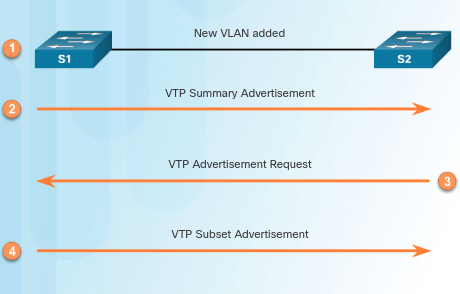
\includegraphics[width=0.6\textwidth]{pictures/VTP-operation.png}
\caption{VTP operation}
\label{VTP-operation}
\end{figure}

\section{VTP Caveats}

Suppose there is a new switch with a higher configuration revision number, and you want to install it into the existing switched network. Then, the existing VLAN configurations will be wiped out (see figure \ref{VTP-caveats}). Therefore, when a switch is added to a network, ensure that it has a default VTP configuration, or its revision number is reset to 0.\\

\begin{figure}[hbtp]
\centering
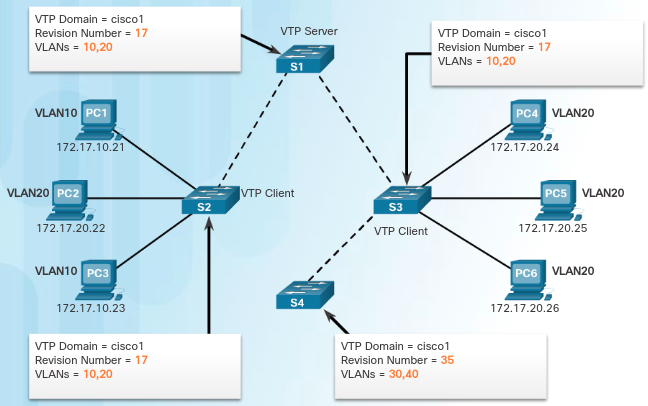
\includegraphics[width=0.8\textwidth]{pictures/VTP-caveats.png}
\caption{Incorrect VTP configuration revision number scenario}
\label{VTP-caveats}
\end{figure}

The VTP configuration revision number is stored in NVRAM and is not reset if you erase switch configuration and reload it. To reset VTP configuration revision number to zero you have two options:

\begin{itemize}
\item Change the switch's VTP domain to a nonexistent VTP domain and then change the domain back to the original name.
\item Change the switch's VTP mode to transparent and then back to previous VTP mode (Recommended).
\end{itemize}

\chapter{STP}
\section{Issues with redundancy}
Multiple cabled paths between switches provide physical redundancy in a switched network. This improves the reliability and availability of the network. However, when there is no spanning tree implementation on the switches, a Layer 2 loop occurs. A Layer 2 loop can result in the three primary issues:
\begin{itemize}
\item Duplicate unicast frames
\item MAC database instability
\item Broadcast storm
\end{itemize}
\subsection{Multiple-frame transmission}
Broadcast frames are not the only type of frames that are affected by loops. Unknown unicast frames sent onto a looped network can result in duplicate frames arriving at the destination device. An unknown unicast frame is when the switch does not have the destination MAC address in its MAC address table and must forward the frame out all ports, except the ingress port.
\subsection{MAC Database Instability}
Ethernet frames do not have a time to live (TTL) attribute. As a result, if there is no mechanism enabled to block continued propagation of these frames on a switched network, they continue to propagate between switches endlessly. \par 
Broadcast frames are forwarded out all switch ports, except the original ingress port. If there is more than one path to the destination, the frames may be forwarded back to the original switch, and create an endless loop. When a loop occurs, the MAC address table on a switch to constantly change with the updates from the broadcast frames, which results in MAC database instability. \par 
See this \href{https://ccnav6.com/s3/course/module2/2.1.1.2/2.1.1.2.html}{link} for more explanation.
\subsection{Broadcast storm}
A broadcast storm occurs when there are so many broadcast frames caught in a Layer 2 loop that all available bandwidth is consumed. Consequently, no bandwidth is available for legitimate traffic and the network becomes unavailable for data communication. This is an effective denial of service (DoS).\par 
There are other consequences of broadcast storms. Because broadcast traffic is forwarded out every port on a switch, all connected devices have to process all the broadcast traffic that is being flooded endlessly around the looped network. This can cause the end device to malfunction because of the processing requirements needed to sustain such a high traffic load on the NIC.
\section{Operation}
\subsection{Port Roles}
IEEE 802.1D STP and RSTP use the Spanning Tree Algorithm (STA) to determine which switch ports on a network must be put in blocking state to prevent loops from occurring. The STA designates a single switch as the root bridge and uses it as the reference point for all path calculations (see figure \ref{STP-operation}). \par 
\begin{figure}[hbtp]
\centering
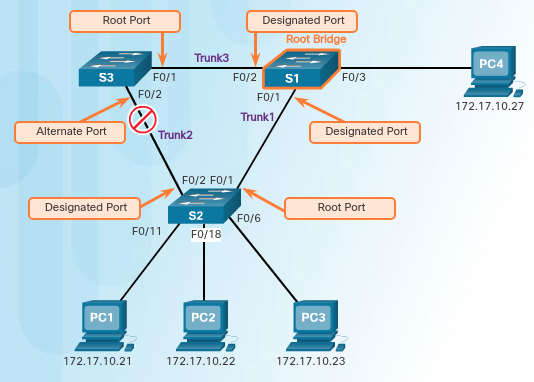
\includegraphics[width=0.8\textwidth]{pictures/STP-operation.png}
\caption{The STA designates a single switch as the root bridge and uses it as the reference point for all path calculations.}
\label{STP-operation}
\end{figure}
After  the root bridge has been determined, the STA calculates the shortest path to the root bridge, while each switch uses the STA to determine which ports to block.  When the STA has determined which paths are most desirable relative to each switch, it assigns port roles to the participating switch ports:
\begin{itemize}
\item \textbf{Root port} -- Switch ports closest to the root bridge in terms of overall cost to the root bridge.
\item \textbf{Designated port} -- All non-root ports that are still permitted to forward traffic on the network.
\item \textbf{Alternate port} -- Alternate ports and backup ports are in discarding or blocking state to prevent loops. 
\end{itemize}
Sometimes, the administrator wants to determine port roles without calculating port cost. He/She should keep in mind the following tips:
\begin{itemize}
\item There can only be one root port per non-root switch
\item If one end of a segment (the link between two switches) is a root port, then the other end is a designated port.
\item All ports on the root bridge are designated ports.
\item Alternate ports are selected only on segments where neither end is a root port.
\end{itemize}
\subsection{Root bridge}
Every switch has its own BID and a root ID:
\subsection{Bridge ID (BID)}
This field is used to uniquely identify the switch in the election process. It includes the priority, extended system ID, and MAC address (see figure \ref{BID}). The bridge priority value is automatically assigned, but can be modified by the administrator. The extended system ID is used to specify a VLAN ID or a multiple spanning tree protocol (MSTP) instance ID. 
\begin{figure}[hbtp]
\centering
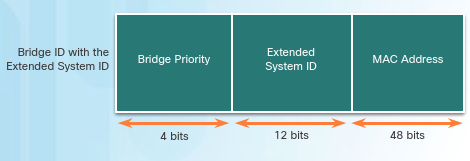
\includegraphics[width=0.6\textwidth]{pictures/BID.png}
\caption{BID fields}
\label{BID}
\end{figure}
The bridge priority is a customizable value that can be used to influence which switch becomes the root bridge. The switch with the lowest priority, which implies the lowest BID, becomes the root bridge because a lower priority value takes precedence. The default priority value for all Cisco switches is the decimal value 32768. The range is 0 to 61440 in increments of 4096.\par 
The extended system ID reserves the rightmost 12 bits for the VLAN ID and the far left 4 bits for the bridge priority. This explains why the bridge priority value can only be configured in multiples of 4096, or $2^12$.\par 
When two switches are configured with the same priority and have the same extended system ID, the switch having the MAC address with the lowest value, expressed in hexadecimal, will have the lower BID. Initially, all switches are configured with the same default priority value. The MAC address is then the deciding factor as to which switch is going to become the root bridge. 
\subsubsection{root ID}
This field indicates the BID of the root bridge. When a switch first boots, the root ID is the same as the bridge ID (BID). However, as the election occurs, the lowest BID replaces the local root ID to identify the root bridge.
\subsubsection{Election process}
All switches in the broadcast domain participate in the election process. After a switch boots, it begins to send out BPDU frames every two seconds. These BPDUs contain the switch BID and the root ID.\par 
Assuming that switch A,B,C,D resides in the same STP domain. As the switch A forward its BPDU frames, adjacent switch B reads the root ID information from the BPDU frames. If the root ID from the BPDU received is lower than the root ID on B, then the B updates its root ID, identifying the A as the root bridge. Switch B then forwards new BPDU frames with the lower root ID to switch C.\par 
The same process repeats, switch C compares its current root ID with the root ID identified in the frames, and then updates its current root ID if needed. Eventually, the switch with the lowest BID ends up being identified as the root bridge for the spanning tree instance.
\subsection{Port role decision}
After the root bridge is elected, the STA determines port roles on interconnecting links.\par 
The root bridge automatically configures all of its switch ports in the designated role. Non-root switches transition ports with the lowest root path cost to root ports, and the other to either  designated or alternate port (because there can only be one root port per non-root switch). \par 
Next step is to decide which port to configure as a designated or alternative port. On the segment, where root ports have already been defined, two switches exchange BPDU frames, which contain the BID. Generally, the switch with the lower BID has its port configured as a designated port while the other has its port configured as an alternate port. However, keep in mind that the first priority is the lowest path cost to the root bridge and that the sender’s BID is used only if the port costs are equal.
\subsection{Root path cost}
The STA considers both path and port costs when determining which ports to block.The path information, known as the internal root path cost, is determined by summing up the individual port costs along the path from the switch to the root bridge. The default port costs are defined by the speed at which the port operates. 10 Gb/s Ethernet ports have a port cost of 2, 1 Gb/s Ethernet ports have a port cost of 4, 100 Mb/s Fast Ethernet ports have a port cost of 19, and 10 Mb/s Ethernet ports have a port cost of 100.\par 
Switches send BPDUs, which include the root path cost. This is the cost of the path from the sending switch to the root bridge. When a switch receives the BPDU, it adds the ingress port cost of the segment to determine its internal root path cost.
\subsection{BPDU frame}
A Bridge Protocol Data Units (BPDU) is a frame exchanged by switches for STP. The spanning tree algorithm depends on the exchange of BPDUs to determine a root bridge. BPDUs have a destination MAC address of 01:80:C2:00:00:00, which is a multicast address for the spanning tree group.  A BPDU frame contains 12 distinct fields:
\begin{itemize}
\item The first four fields identify the protocol, version, message type, and status flags.
\item The next four fields are \textit{root ID}, \textit{bridge ID (BID)}, root path cost. They are  used to identify the root bridge and the root path cost to the root bridge.
\item The last four fields are all timer fields that determine how frequently BPDU messages are sent and how long the information received through the BPDU process is retained.
\end{itemize}
\section{Types of STP}
\begin{itemize}
\item \textbf{STP} -- This is the original IEEE 802.1D version. The protocol assumes one spanning tree instance for the entire bridged network.
\item \textbf{PVST+} -- This is a Cisco enhancement of STP that provides a separate 802.1D spanning tree instance for each VLAN configured in the network.
\item \textbf{802.1D-2004} -- This is an updated version of the STP standard, incorporating IEEE 802.1w.
\item \textbf{RSTP or IEEE 802.1w} -- This is an evolution of STP.
\item \textbf{Rapid PVST+} -- This is a Cisco enhancement of RSTP that uses PVST+.
\item \textbf{MSTP} -- Multiple Spanning Tree Protocol. This is an IEEE standard inspired by the earlier Cisco proprietary Multiple Instance STP (MISTP) implementation. MSTP maps multiple VLANs into the same spanning tree instance. The Cisco implementation of MSTP is MST, which provides up to 16 instances of RSTP
\end{itemize}
\subsection{Port states and PVST+ Operation}
To facilitate the learning of the logical spanning tree, each switch port transitions through five possible port states and three BPDU timers:
\begin{table}[h!]
\centering
\caption{Five port states in PVST+}
\label{PVST-port-state}
\begin{tabular}{|p{0.25\textwidth}|l|l|l|l|l|}
\hline
                                                    & \multicolumn{5}{c|}{Port states}                        \\ \hline
Operation allowed                                   & Blocking & Listening & Learning & Forwarding & Disabled \\ \hline
Learn MAC addresses                                 & YES      & YES       & YES      & YES        & NO       \\ \hline
Forward data frames received on interface           & NO       & NO        & YES      & YES        & NO       \\ \hline
Forward data frames switched from another interface & NO       & NO        & NO       & YES        & NO       \\ \hline
Receive and process BPDUs                           & NO       & NO        & NO       & YES        & NO       \\ \hline
\end{tabular}
\end{table}
\subsection{Rapid PVST+}
Rapid PVST+ is the Cisco implementation of RSTP on a per-VLAN basis. An independent instance of RSTP runs for each VLAN.\par 
RSTP does not have a blocking port state. Port states are defined as discarding, learning, or forwarding. RSTP also speeds the recalculation of the spanning tree when the Layer 2 network topology changes. If a port is configured to be an alternate port or a backup port, it can immediately change to a forwarding state without waiting for the network to converge.\par 
RSTP introduces new types of port: edge port. An RSTP edge port is a switch port that is never intended to be connected to another switch. It immediately transitions to the forwarding state when enabled. The RSTP edge port concept corresponds to the PVST+ PortFast feature. An edge port is directly connected to an end station and assumes that no switch device is connected to it.
\chapter{EtherChannel}
\section{Introduction}
\subsection{Advantages}
EtherChannel technology has many advantages:
\begin{itemize}
\item Most configuration tasks can be done on the EtherChannel interface instead of on each individual port, ensuring configuration consistency throughout the links.
\item EtherChannel creates an aggregation that is seen as one logical link. 
\item EtherChannel provides redundancy.
\item Load balancing takes place between links that are part of the same EtherChannel. 
\item EtherChannel relies on existing switch ports. There is no need to upgrade the link to a faster and more expensive connection to have more bandwidth.
\end{itemize}
\subsection{Implementation restrictions}
The EtherChannel provides full-duplex bandwidth between one switch and another switch or host. Currently each EtherChannel can consist of up to eight compatibly-configured Ethernet ports. However, interface types cannot be mixed. For example, Fast Ethernet and Gigabit Ethernet cannot be mixed within a single EtherChannel.\par 
EtherChannel creates a one-to-one relationship; that is, one EtherChannel link connects only two devices. The individual EtherChannel group member port configuration must be consistent on both devices. It is mandatory that all ports have the same speed, duplex setting, and VLAN information. Any port modification after the creation of the channel also changes all other channel ports. If the physical ports of one side are configured as trunks, the physical ports of the other side must also be configured as trunks within the same native VLAN. Additionally, all ports in each EtherChannel link must be configured as Layer 2 ports. 

\section{Port Aggregation Protocol (PagP)}
PAgP (pronounced “Pag – P”) is a Cisco-proprietary protocol that aids in the Passivematic creation of EtherChannel links. PAgP helps create the EtherChannel link by detecting the configuration of each side and ensuring that links are compatible so that the EtherChannel link can be enabled when needed. PAgP can be configured in one of three models:
\begin{itemize}
\item \textbf{On} -- This mode forces the interface to channel without PAgP. Interfaces configured in the on mode do not exchange PAgP packets.
\item \textbf{PAgP Active} -- This PAgP mode places an interface in an active negotiating state in which the interface initiates negotiations with other interfaces by sending PAgP packets.
\item \textbf{PAgP Passive} -- This PAgP mode places an interface in a passive negotiating state in which the interface responds to the PAgP packets that it receives, but does not initiate PAgP negotiation.
\end{itemize}
The modes must be compatible on each side as shown in table \ref{PAgP-mode}.
\begin{table}[htbp]
\caption{PAgP Establishment}
\label{PAgP-mode}
\begin{tabular}{|l|l|l|}
\hline
S1             & S2                & EtherChannel establishment \\ \hline
Active      & Passive/Active    & Yes                        \\ \hline
On             & On                & Yes                        \\ \hline
Passive           & Passive/On           & No                         \\ \hline
Not configured & Passive/Active/On & No                         \\ \hline
Active      & on                & No                         \\ \hline
\end{tabular}
\end{table}
\section{Link Aggregation Control Protocol (LACP)}
LACP is part of an IEEE specification (802.3ad) that allows several physical ports to be bundled to form a single logical channel. Because LACP is an IEEE standard, it can be used to facilitate EtherChannels in multivendor environments, including Cisco devices. LACP allows for eight active links, and also eight standby links. A standby link will become active should one of the current active links fail.
PAgP can be configured in one of three models:
\begin{itemize}
\item \textbf{On} -- This mode forces the interface to channel without LACP. Interfaces configured in the on mode do not exchange LACP packets.
\item \textbf{LACP active} -- Similar to PAgP Active mode.
\item \textbf{LACP passive} -- Similar to PAgP Passive mode. negotiation.
\end{itemize}
The modes must be compatible on each side as shown in table \ref{PAgP-mode}.
\begin{table}[htbp]
\caption{LACP Establishment}
\label{LACP-mode}
\begin{tabular}{|l|l|l|}
\hline
S1             & S2                & EtherChannel establishment \\ \hline
Active      & Passive/Active    & Yes                        \\ \hline
On             & On                & Yes                        \\ \hline
Passive           & Passive/On           & No                         \\ \hline
Not configured & Passive/Active/On & No                         \\ \hline
Active      & on                & No                         \\ \hline
\end{tabular}
\end{table}

\section{Configuration}


\part{ROUTING TECHNOLOGIES}
\chapter{Router}

The primary function of a router is: Determine the best path to send packets and Forward packets toward their destination.

\section{Packet-Forwarding Mechanisms}

\begin{itemize}
\item \textbf{Process switching:} Process switching starts finding a path every time a packet arrives, even if the destination is the same for a stream of packets. This mechanism is slow and old-fashioned.

\item \textbf{Fast switching:} The flow information for the packet is also stored in the \emph{fast-switching cache}. If another packet going to the same destination arrives on an interface, the next-hop information in the cache is reused without CPU intervention.

\item \textbf{Cisco Express Forwarding (CEF):} CEF builds a Forwarding Information Base (FIB), and an adjacency table, then stores them in the data plane. The FIB contains precomputed reverse lookups, next-hop information for routes including the interface, and Layer 2 information. Therefore, when a network has converged, the FIB and adjacency tables contain all the information a router would have to consider when forwarding a packet. This enables forwarding of packets to occur at the data plane without consulting the control plane.
\end{itemize}

\section{Router Switching Function}

The router performs the following three major steps (Figure \ref{SwitchingFunc}):

\begin{figure}[hbtp]
\caption{Encapsulating and De-encapsulating packets}\label{SwitchingFunc}
\centering
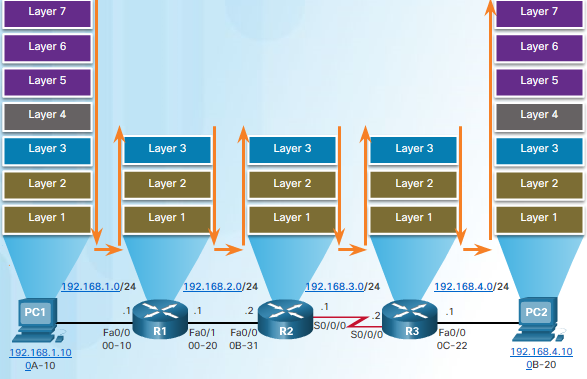
\includegraphics[scale=0.7]{pictures/SwitchingFunc.PNG}
\end{figure}


\begin{enumerate}
\item De-encapsulates the Layer 2 frame header and trailer to expose the Layer 3 packet.

\item Examines the destination IP address of the IP packet to find the best path in the routing table.

\item If the router finds a path to the destination, it encapsulates the Layer 3 packet into a new Layer 2 frame and forwards the frame out the exit interface. MAC addresses are only required on Ethernet multiaccess networks. A serial link is a point-to-point connection and uses a different Layer 2 frame that does not require the use of a MAC address. Because there are no MAC addresses on serial interfaces, a router sets the data link destination address to an equivalent of a broadcast.
\end{enumerate}

\section{Path determination}

A metric is the quantitative value used to measure the distance to a given network. The best path to a network is the path with the lowest metric. The following lists some dynamic protocols and the metrics they use:

\begin{itemize}
\item RIP -- hop count
\item OSPF -- bandwidth
\item EIGRP -- Bandwidth, delay, load, reliability
\end{itemize}

When a router has two or more paths to a destination with equal cost metrics, then the router forwards the packets using both paths equally. This is called equal cost \textbf{load balancing}. The routing table contains the single destination network but has multiple exit interfaces, one for each equal cost path. Only \emph{EIGRP} supports \emph{unequal cost load balancing}.\\

A router uses what is known as the \textbf{administrative distance (AD)} to determine the route to install into the IP routing table. The AD represents the trustworthiness of the route; the lower the AD, the more trustworthy the route source. For example, when a router has the choice of a static route (AD = 1) and an EIGRP route (AD = 90), the static route takes precedence. The following list shows the AD value of common routes:

\begin{itemize}
\item Connected interface = 0
\item Static route = 1
\item BGP = 20
\item Internal EIGRP = 90
\item OSPF = 110
\item RIP = 120
\item External EIGRP = 170
\item Internal BGP = 200
\end{itemize}
\chapter{IPv6}

\section{Representation}

IPv6 addresses are 128 bits in length and written as a string of 32 hexadecimal values. Every 4 bits is represented by a single hexadecimal digit. The preferred format for writing an IPv6 address is x:x:x:x:x:x:x:x, where each ``x'' is a single \emph{hextet}\footnote{four hexadecimal values}. For example,

\begin{verbatim}
2001:0DB8:0000:1111:0000:0000:0000:0200
\end{verbatim}

There are two rules to help reduce the number of digits needed to represent an IPv6 address.

\begin{itemize}
\item \textbf{Omit leading 0s:} Omit any leading 0s (zeros) in any hextet. This rule only applies to leading 0s, NOT to trailing 0s; otherwise, the address would be ambiguous. For example, the hextet \verb|0ABC| will become \verb|ABC|.

\begin{verbatim}
2001:0DB8:0000:1111:0000:0000:0000:0200
2001: DB8:   0:1111:   0:   0:   0: 200
\end{verbatim}

\item \textbf{Omit 0 segments:} Double colon (::) can replace any contiguous string of one or more hextets consisting of all 0s. The double colon (::) can only be used once within an address; otherwise, there would be more than one possible resulting address. 

\begin{verbatim}
2001:0DB8:0000:1111:0000:0000:0000:0200
2001: DB8:   0:1111:   0:   0:   0: 200
2001: DB8:   0:1111::200
\end{verbatim}
\end{itemize}

\section{Types of IPv6 Addresses}

There are three types of IPv6 addresses: Unicast, Multicast, and Anycast. Unlike IPv4, IPv6 does not have a broadcast address. However, there is an IPv6 all-node multicast address that essentially gives the same result.

\subsection{Unicast IPv6}

An IPv6 unicast address uniquely identifies an interface on an IPv6-enabled device. There are three types of IPv6 unicast address: Global unicast, Link-local and Unique local unicast.

\paragraph{Global unicast:} A global unicast address  is a globally unique and Internet-routable address. The ICANN\footnote{Internet Committee for Assigned Names and Numbers} assigns IPv6 Global Unicast address to organization. A global unicast address has three parts: Global routing prefix, Subnet ID, Interface ID (Figure \ref{GUA}). The \textbf{global routing prefix} (first three hextets) is the network portion of the IPv6 address that is assigned by the ISP. The \textbf{Subnet ID} (fourth hextet) is used by an organization to identify subnets within its site. The \textbf{Interface ID} (last four hextets) is the host portion of the address.

\begin{figure}[hbtp]
\caption{Global routing prefix}\label{GUA}
\centering
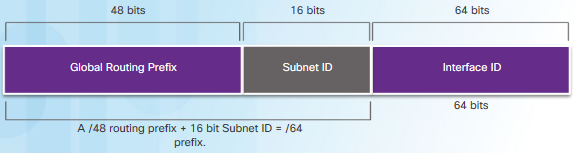
\includegraphics[scale=0.6]{pictures/GUA.PNG}
\end{figure}


\paragraph{Link-local:} Link-local addresses are used to communicate with other devices on the same local link\footnote{With IPv6, the term link refers to a subnet.}. Packets with a source or destination link-local address cannot be routed beyond the link from which the packet originated. Their uniqueness must only be confirmed on that link. If a link-local address is not configured manually on an interface, the device will automatically create its own. IPv6 link-local addresses are in the FE80::/10 range\footnote{The /10 indicates that the first 10 bits are 1111 1110 10xx xxxx. The first hextet has a range of 1111 1110 1000 0000 (FE80) to 1111 1110 1011 1111 (FEBF)}.

\paragraph{Dynamic Link-Local Addresses} A link-local address can be established dynamically or configured manually as a static link-local address. Operating systems will typically use either EUI-64 process or a randomly generated 64-bit
number to dynamically assign link-local address. By default, Cisco routers use EUI-64 to generate the Interface ID for all link-local address on IPv6 interfaces. For serial interfaces, the router will use the MAC address of an Ethernet interface.

\paragraph{Static Link-Local Addresses} A drawback to using the dynamically assigned link-local address is its long interface ID, which makes it challenging to identify and remember assigned addresses. Configuring the link-local address manually provides the ability to create an address that is recognizable and easier to remember.

\begin{verbatim}
R1(config)# interface g0/0
R1(config-if)# ipv6 address fe80::1 link-local
\end{verbatim}

The link-local address in the above example is used to make it easily recognizable as belonging to router R1. The same IPv6 link-local address is configured on all of R1's interfaces. FE80::1 can be configured on each link because it only has to be unique on that link. Similar to R1, router R2 would be configured with FE80::2 as the IPv6 link-local address on all of its interfaces

\paragraph{Unique local unicast:}Unique local addresses are used for local addressing within a site or between a limited number of sites. These addresses should not be Internet-routable and should not be translated to a global IPv6 address. Unique local addresses can be used for devices that will never need or have access from another network. Unique local addresses are in the range of FC00::/7 to FDFF::/7.

\subsection{Multicast IPv6}

IPv6 multicast addresses have the prefix FF00::/8. Multicast addresses can only be destination addresses and not source addresses. There are two types of IPv6 multicast addresses: Assigned multicast address and Solicited node multicast address.

\paragraph{Assigned mulicast addresses} are reserved multicast addresses for predefined groups of devices. For example, FF02::1 is the all-nodes multicast address, which has the same effect as broadcast IPv4 address. The all-routers multicast address FF02::2 identifies a group of all IPv6 routers\footnote{A router with the ipv6 unicast-routing global configuration command executed} on the network.

\paragraph{A solicited-node multicast address} is mapped to a special Ethernet multicast address. This allows the Ethernet NIC to filter the frame by examining the destination MAC address.

\section{ICMPv6}

\subsection{Description}

The informational and error messages found in ICMPv6 are very similar to the control and error messages implemented by ICMPv4. However, ICMPv6 has new features and improved functionality not found in ICMPv4. ICMPv6 includes four types of message: RS and RA message\footnote{Router Solicitation (RS) message, Router Advertisement (RA) message} (communication between a router and a device), NS and NA message\footnote{Neighbor Solicitation (NS) message, Neighbor Advertisement (NA) message} (communication between devices). Address resolution and DAD process use NA and NS message, while RS and RA message contribute to assigning IPv6 to devices.\\

\begin{figure}[hbtp]
\caption{Address Resolution}\label{AddressResolution}
\centering
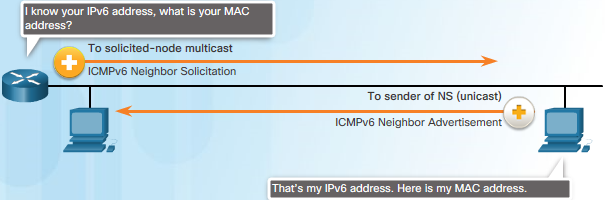
\includegraphics[scale=1]{pictures/AddressResolution.PNG}
\end{figure}


\paragraph{Address resolution} acts like ARP of IPv4. It is used to determine the MAC address of a destination IPv6 address. A device will send an NS message to the solicited node address to ask for MAC address. The message will include the known (targeted) IPv6 address. The device that has the targeted IPv6 address will respond with an NA message containing its Ethernet MAC address. Figure \ref{AddressResolution} shows two PCs exchanging NS and NA messages.

\begin{figure}[hbtp]
\caption{DAD process}\label{DADprocess}
\centering
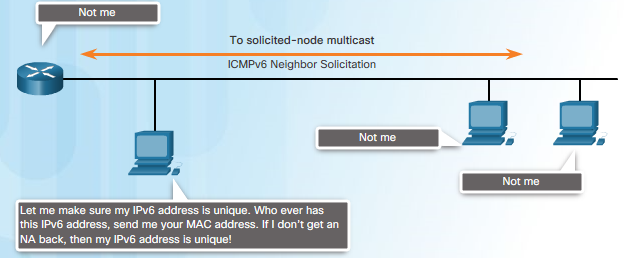
\includegraphics[scale=1]{pictures/DADprocess.PNG}
\end{figure}


\paragraph{DAD process} is a Duplicate Address Detection.  To check the uniqueness of an address, the device will send an NS message with its own IPv6 address as the targeted IPv6 address, shown in Figure \ref{DADprocess}. If another device on the network has this address, it will respond with an NA message. This NA message will notify the sending device that the address is in use. If a corresponding NA message is not returned within a certain period of time, the unicast address is unique and acceptable for use.

\subsection{Traceroute}

Traceroute (tracert) is a utility that generates a list of hops that were successfully reached along the path. Traceroute uses ICMP to accomplish its purpose.\\

Using traceroute provides round trip time for each hop along the path and indicates if a hop fails to respond. The round trip time is the time a packet takes to reach the remote host and for the response from the host to return. An asterisk (*) is used to indicate a lost or unreplied packet.\\

Traceroute makes use of a function of the TTL field in IPv4 and the Hop Limit field in IPv6 along with the ICMP time-exceeded message. The first sequence of messages sent from traceroute will have a TTL field value of 1. This causes the TTL to timeout the IPv4 packet at the first router. This router then responds with an ICMPv4 message. Traceroute now has the address of the first hop. Traceroute then progressively increments the TTL field (2, 3, 4, ...) to get the address of the next hops.\\

After the final destination is reached, the host responds with either an ICMP port \emph{unreachable} message or an ICMP \emph{echo reply} message instead of the ICMP time exceeded message.

\section{EUI-64 Process}

When the RA message is either SLAAC or SLAAC with stateless DHCPv6, the client must generate its own Interface ID using EUI-64 Process or Randomly Generated. An EUI-64 Interface ID is represented in binary and is made up of three parts (Figure \ref{EUI64}):

\begin{itemize}
\item \textbf{24-bit OUI} from the client MAC address\footnote{Ethernet MAC addresses are made up of two parts: vendor code OUI assigned by IEEE and device identifier}, but the 7th bit (the Universally/Locally (U/L) bit) is reversed. This means that if the 7th bit is a 0, it becomes a 1, and vice versa.
\item The inserted 16-bit value \textbf{FFFE} (in hexadecimal).
\item \textbf{24-bit Device Identifier} from the client MAC address.
\end{itemize}

\begin{figure}[hbtp]
\caption{EUI-64 process}\label{EUI64}
\centering
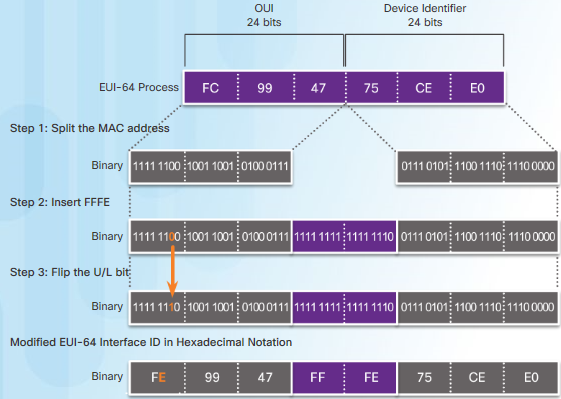
\includegraphics[scale=1]{pictures/EUI64.PNG}
\end{figure}

The advantage of EUI-64 is the Ethernet MAC address can be used to determine the Interface ID. It also allows network administrators to easily track an IPv6 address to an end device using the unique MAC address. However, this has caused privacy concerns among many users. They are concerned that their packets can be traced to the actual physical computer. Due to these concerns, a randomly generated Interface ID may be used instead. 

\section{IPv4 and IPv6 Coexistence}

Several techniques have been developed to accommodate a variety of transition IPv4-to-IPv6 scenarios:

\begin{itemize}
\item \textbf{Dual-stack:} A device interface is running both IPv4 and IPv6 protocols enabling it to communicate with either network.
\item \textbf{Tunneling:} The process of encapsulating an IPv6 packet inside an IPv4 packet. This allows the IPv6 packet to be transmitted over an IPv4-only network.
\item \textbf{Translation:} NAT64 allows IPv6-enabled devices to communicate with IPv4-enabled devices using a translation technique similar to NAT for IPv4. An IPv6 packet is translated to an IPv4 packet and vice versa.
\end{itemize}
\chapter{Static routing}

\section{Overview}

\begin{table}[hbtp]
\centering\caption{Dynamic vs Static routing}
\begin{tabular}{ p{2cm} p{8cm} p{8cm} }
\toprule
\head{Feature} & \head{Dynamic routing} & \head{Static routing} \\
\midrule

Configuration complexity & Independent of network size & Increase with network size \\

Topology changes & Automatically adapt to changes & Administrator intervention required \\

Usage & Complex and growing network, normal route & Small network, Stub network, default route, summary route, backup route \\

Resource & CPU, memory, bandwidth & No resources needed \\

Predictability & Depends on current topology & Always the same \\

Security & Advertise protocol message over the entire network, resulting security risk & Not advertised over the network, resulting in better security \\

Configuration & simple, nearly error-free & error-prone, require complete knowledge of the whole network for proper configuration \\

\bottomrule
\end{tabular}
\end{table}

\section{IPv4 route configuration}

Static routes are configured using the \verb|ip route| global configuration command. The basic syntax for the command is as follows:

\begin{verbatim}
Router(config)# ip route network-addr subnet-mask {ip-address | exit-intf} [distance]
\end{verbatim}

The \verb|network-addr| and \verb|subnet-mask| are the IP address and subnet mask of the destination network. The \verb|distance| parameter specifies AD. By default, static route has AD of 1.\\

The next hop can be identified by an IP address (\verb|ip-address|), exit interface (\verb|exit-intf|), or both. The way the destination is specified creates one of the three following route types:

\begin{itemize}
\item \textbf{Next-hop} static route: Only the next-hop IP address is specified.

\begin{verbatim}
R1(config)# ip route 172.16.1.0 255.255.255.0 172.16.2.2
\end{verbatim}

\item \textbf{Directly connected} static route: Only the router exit interface is specified.

\begin{verbatim}
R1(config)# ip route 172.16.1.0 255.255.255.0 s0/0/0
\end{verbatim}

\item \textbf{Fully specified} static route: The next-hop IP address and exit interface are specified. When the exit interface is a multiaccess network (e.g. Ethernet network), it is recommended that a fully specified static route be used. 

\begin{verbatim}
R1(config)# ip route 172.16.1.0 255.255.255.0 g0/0 172.16.2.2
\end{verbatim}
\end{itemize}

A route that does not reference an exit interface must perform a \emph{recursive lookup}. Recursive lookup means that the router searches through the routing table to find the interface that match the next-hop IP address. 

Along with \verb|ping| and \verb|traceroute|, useful commands to verify static routes include these:
\begin{verbatim}
R1# show ip route
R1# show ip route static
R1# show ip route 192.168.1.0
R1# show running-config | section ip route
\end{verbatim}

\section{IPv6 route configuration}

The \verb|ipv6 unicast-routing| global configuration command must be configured to enable the router to forward IPv6 packets. Static routes for IPv6 are configured using the \verb|ipv6 route| global configuration command. The syntax is as follows:

\begin{verbatim}
Router(config)# ipv6 route ipv6-prefix/prefix-length {ipv6-address | exit-intf}

R1(config)# ipv6 route 2001:DB8:ACAD:2::/64 2001:DB8:ACAD:4::2
R1(config)# ipv6 route 2001:DB8:ACAD:2::/64 s0/0/0
R1(config)# ipv6 route 2001:db8:acad:2::/64 s0/0/0 fe80::2
\end{verbatim}

\note  If the IPv6 static route uses an IPv6 link-local address as the next-hop address, a fully specified static route including the exit interface must be used.\\

Along with \verb|ping| and \verb|traceroute|, useful commands to verify static routes include these:

\begin{verbatim}
R1# show ipv6 route
R1# show ipv6 route static
R1# show ipv6 route 2001:db8:acad:3::
R1# show running-config | section ipv6 route
\end{verbatim}

\section{Types}

There are four types static routes: Standard, Default, Summary, and Floating.

\subsection{IPv4 Default static route}  

A default route is used when no other routes in the routing table match the destination IP address of the packet. It acts as the Gateway of Last Resort. The command syntax for a default static route is similar to any other static route, except that the network address is \verb|0.0.0.0| and the subnet mask is \verb|0.0.0.0|.

\begin{verbatim}
R1(config)# ip route 0.0.0.0 0.0.0.0 172.16.2.2
\end{verbatim}

Note the asterisk (*) next to the route with code \verb|S| in the output of the \verb|show| command. The asterisk indicates that this static route is a candidate default route, which is why it is selected as the Gateway of Last Resort.

\begin{verbatim}
R1# show ip route static
<output omitted>
Gateway of last resort is 172.16.2.2 to network 0.0.0.0
S* 0.0.0.0/0 [1/0] via 172.16.2.2
\end{verbatim}

\subsection{IPv6 Default static route}  

Unlike IPv4, IPv6 does not explicitly state that the default IPv6 is the Gateway of Last Resort. The command syntax for a default static route is similar to any other static route, except that the ipv6-prefix/prefix-length is \verb|::/0|, which matches all routes.

\begin{verbatim}
Router(config)# ipv6 route ::/0 {ipv6-address | exit-intf}
R1(config)# ipv6 route ::/0 2001:DB8:ACAD:4::2
\end{verbatim}

\subsection{Summary static route}

To reduce the number of routing table entries, multiple static routes can be summarized into a single static route in the following circumstances:

\begin{itemize}
\item The destination networks are contiguous and can be summarized into a single network address.
\item All the multiple static routes use the same exit interface or next-hop IP address.
\end{itemize}

\paragraph{Floating static route}

Floating static routes are static routes that are used to provide a backup path, in the event of a link failure. This route is only used when the primary route is not available. To accomplish this, the floating static route is configured with a higher AD\footnote{The AD represents the trustworthiness of a route. If multiple paths to the destination exist, the router will choose the path with the lowest AD.} than that of another static route or dynamic routes. The floating route is not shown in the routing table until the primary route is not available.

\begin{verbatim}
R1(config)# ip route 0.0.0.0 0.0.0.0 10.10.10.2 5
R3(config)# ipv6 route ::/0 2001:db8:acad:6::2 5
\end{verbatim}

\subsection{Static host routes}

A host route is an IPv4 address with a 32-bit mask or an IPv6 address with a 128-bit mask. There are three ways a host route can be added to the routing table:

\begin{itemize}
\item Automatically installed when an IP address is configured on the router
\item Configured as a static host route
\item Host route automatically obtained through other methods (discussed in
\end{itemize}

Cisco IOS automatically installs a host route, also known as a \emph{local host route}, when an interface address is configured on the router. A host route allows for a more efficient process for packets that are directed to the router itself, rather than for packet forwarding. This is in addition to the connected route, designated with a C in the routing table for the network address of the interface.

\begin{verbatim}
Branch# show ip route
Gateway of last resort is not set
    198.51.100.0/24 is variably subnetted, 2 subnets, 2 masks
C     198.51.100.0/30 is directly connected, Serial0/0/0
L     198.51.100.1/32 is directly connected, Serial0/0/0

Branch# show ipv6 route
C     2001:DB8:ACAD:1::/64 [0/0]
        via Serial0/0/0, directly connected
L     2001:DB8:ACAD:1::1/128 [0/0]
        via Serial0/0/0, receive
\end{verbatim}

A host route can be a manually configured static route to dire ct traffic to a specific destination device, such as an authentication server.

\begin{verbatim}
Branch(config)# ip route 209.165.200.238 255.255.255.255 198.51.100.2
Branch(config)# ipv6 route 2001:db8:acad:2::99/128 2001:db8:acad:1::2
Branch(config)# ipv6 route 2001:db8:acad:2::99/128 s0/0/0 fe80::2
\end{verbatim}
\chapter{EIGRP}

\section{Basic features}

Enhanced Interior Gateway Routing Protocol (EIGRP) is a powerful \emph{distance vector} routing protocol and is relatively easy to configure for basic networks. Features of EIGRP:

\begin{itemize}
\item Use DUAL algorithm
\item Use RTP  instead of TCP or UDP
\item Partial and Bounded Updates -- Sends updates only when there is a change and only to the routers that need the information
\item Supports Equal and Unequal cost load balancing
\item Does not encrypt the routing updates
\item \textbf{Authentication:} Only accepts routing information from other routers with the same authentication information 
\end{itemize}

\paragraph{Protocol Dependent Modules (PDM)}sends and receives EIGRP packets that are encapsulated in IPv4 or IPv6.

\paragraph{Reliable Transport Protocol (RTP)}EIGRP was designed as a network layer independent routing protocol. Because of this design, EIGRP cannot use UDP or TCP, but use RTP instead. RTP includes both reliable and unreliable delivery of EIGRP packets, similar to TCP and UDP, respectively. RTP can send EIGRP packets as unicast or multicast. EIGRP multicast address is 224.0.0.10 for IPv4 and  FF02::A for IPv6.

\section{Packet types}

\subsection{Hello packets}

EIGRP uses small Hello packets to discover other EIGRP-enabled routers on directly connected links. Hello packets are used by routers to form EIGRP neighbor adjacencies.\\
 
Hello packets are sent as multicast packets \emph{every five seconds}. However, on slow network (e.g. multipoint, NBMA networks with access links of T1), Hello packets are sent as unicast packets every 60 seconds.\\
 
EIGRP uses a Hold timer to determine the maximum time the router should wait to receive the next Hello before declaring that neighbor as unreachable. By default, the Hold timer is \emph{three times the Hello interval}. If the hold time expires, EIGRP declares the route as down and DUAL searches for a new path by sending out queries.\\

Hello intervals and hold times are configurable on a per-interface basis and \emph{do not have to match} with other EIGRP routers to establish or maintain adjacencies. If the Hello interval is changed, ensure that the Hold time value is not less than the Hello interval. Otherwise, neighbor adjacency goes down after the Hold timer expires and before the next Hello interval. 

\subsection{Update packets}

EIGRP sends Update packets to propagate routing information. Update packets are sent only when necessary. EIGRP updates contain only the routing information needed, and are sent only to those routers that require it.\\
 
EIGRP uses \emph{partial update} and \emph{bounded update}. A partial update means that the update only includes information about route changes. A bounded update refers to the sending of partial updates only to the routers that are affected by the changes. Bounded updates help EIGRP minimize the bandwidth that is required to send EIGRP updates.

\subsection{Acknowledgment packets}

EIGRP sends Acknowledgment (ACK) packets when RTP reliable delivery is used. An EIGRP acknowledgment is an EIGRP Hello packet without any data. RTP uses reliable delivery for Update, Query, and Reply packets.

\subsection{Query and reply packets}

DUAL uses Query and Reply packets when searching for networks and other tasks. Queries can use multicast or unicast, whereas replies are always sent as unicast.

\section{Encapsulating EIGRP Messages}
The EIGRP packet headers and TLV (Type, Length, Value) field are encapsulated in an IP packet.

\subsection{IP packet header}

In the IP packet header (figure \ref{EIGRP-packet-header}), the protocol field is set to \textbf{88} to indicate EIGRP. The destination address is set to the multicast 224.0.0.10 for IPv4, and FF02::A for IPv6. If the EIGRP packet is encapsulated in an Ethernet frame, the destination MAC address is the multicast address 01-00-5E-00-00-0A.

\subsection{EIGRP packet header}

\begin{figure}[hbtp]
\centering
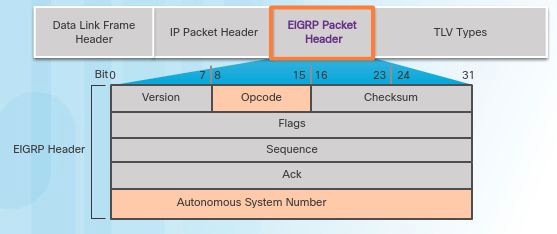
\includegraphics[width=0.6\textwidth]{pictures/EIGRP-packet-header.png}
\caption{EIGRP packet header} \label{EIGRP-packet-header}
\end{figure}

\paragraph{Opcode field} specifies EIGRP packet type. Specifically, it identifies the EIGRP messages as either Update (1), Query (3), Reply (4), and Hello (5).\\
 
\paragraph{Autonomous system (AS) number}specifies the EIGRP routing process. Unlike RIP, multiple instances of EIGRP can run on a network. The autonomous system number is used to track each running EIGRP process.

\subsection{TLV fields}

There are three types of TLV: EIGRP parameters (figure \ref{EIGRP-parameters}), IP internal routes (figure \ref{EIGRP-internal-route}), and IP external routes (figure \ref{EIGRP-external-route}).\\

\begin{figure}[hbtp]
\centering
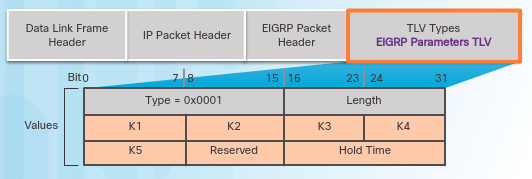
\includegraphics[width=0.6\textwidth]{pictures/EIGRP-parameters.png}
\caption{EIGRP TLV: EIGRP parameters} \label{EIGRP-parameters}
\end{figure}

The \emph{length} field identifies the size (in bytes) of the \emph{value} field. The \emph{value} field contains data for EIGRP message. The \emph{type} field specifies the type of TLV: EIGRP parameters (1), IP internal routes (258), and IP external routes (259).\\

\begin{figure}[hbtp]
\centering
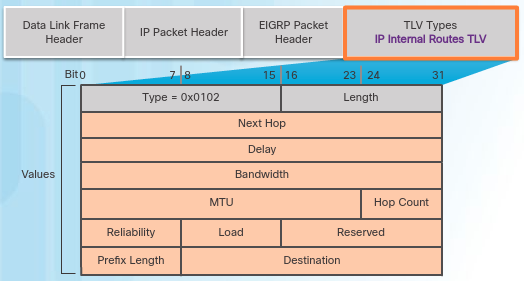
\includegraphics[width=0.6\textwidth]{pictures/EIGRP-internal-route.png}
\caption{EIGRP internal routes TLV fields} \label{EIGRP-internal-route}
\end{figure}

The EIGRP parameters include the weights that EIGRP uses for its composite metric (K1 -- K5). By default, only bandwidth and delay are weighted. Both are weighted equally; therefore, the K1 field for bandwidth and the K3 field for delay are both set to one (1). The other K values are set to zero (0).\\

\begin{figure}[hbtp]
\centering
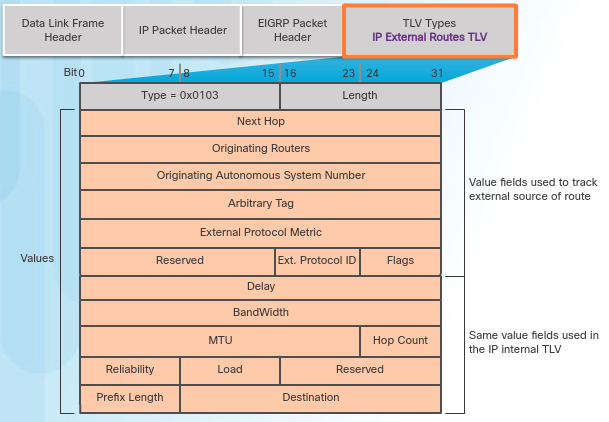
\includegraphics[width=0.6\textwidth]{pictures/EIGRP-external-route.png}
\caption{EIGRP external route TLV fields} \label{EIGRP-external-route}
\end{figure}
 
Each IP internal route or IP external route contains one route entry and the metric information for specific route. These types of TLV are included in EIGRP Update packets. The IP internal route message is used to advertise EIGRP routes within an autonomous system. The IP external message is used to import default static route, as well as routes outside the autonomous system, into the EIGRP routing process.
 
\section{Operation}

\subsection{Neighbor adjacency}
EIGRP uses Hello packets to establish and maintain neighbor adjacencies. To accomplish this, two EIGRP routers must use the same K values and autonomous system number.\\

\begin{figure}[hbtp]
\caption{Establish EIGRP adjacency}\label{EIGRPadjacency}
\centering
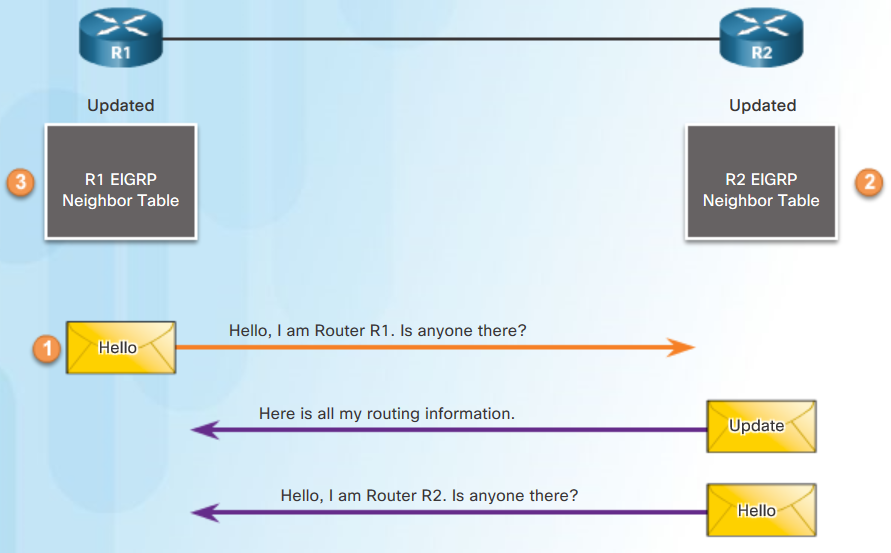
\includegraphics[scale=0.6]{pictures/EIGRPadjacency.PNG}
\end{figure}

 
Each EIGRP router maintains a neighbor table, which contains a list of routers that have an EIGRP adjacency with this router. The neighbor table is used to track the status of these EIGRP neighbors.\\

Figure \ref{EIGRPadjacency} shows two EIGRP routers exchanging initial EIGRP Hello packets. When an EIGRP enabled router receives a Hello packet on an interface, it adds that router to its neighbor table:

\begin{enumerate}
\item A new router (R1) comes up on the link and sends an EIGRP Hello packet through all of its EIGRP-configured interfaces.

\item Router R2 receives the Hello packet on an EIGRP-enabled interface. R2 replies with an EIGRP update packet that contains all the routes it has in its routing table, except those learned through that interface (split horizon). However, the neighbor adjacency is not established until R2 also sends an EIGRP Hello packet to R1.

\item After both routers have exchanged Hellos, the neighbor adjacency is established. R1 and R2 update their EIGRP neighbor tables adding the adjacent router as a neighbor.
\end{enumerate}

\subsection{Topology table}

The topology table includes all destinations advertised by neighboring (adjacent) routers and the cost (metric) to reach each network. When a router receives the EIGRP update from a neighbor, it adds all update entries to its topology table. Because EIGRP update packets use RTP reliable delivery, the router replies with an EIGRP acknowledgment packet.

\subsection{Metric}

By default, EIGRP uses the following values in its composite metric to calculate the preferred path to a network:

\begin{itemize}
\item \textbf{Bandwidth} -- The slowest bandwidth among all of the outgoing interfaces, along the path from source to destination.
\item \textbf{Delay} -- The cumulative (sum) of all interface delay along the path (in tens of microseconds).
\end{itemize}

Default composite formula:
\[ \text{metric} = \left( \text{bandwidth} + \text{bandwidth} \right) \times 256 \]

Complete composite formula:
\[ \text{metric} = \left( K1\times\text{bandwidth} + \frac{K2\times\text{bandwidth}}{256\times\text{load}} + K3\times\text{delay} \right) \times \frac{K5}{K4+\text{reliability}} \times 256 \]
This is a conditional formula. If $K5=0$, the last term is replaced by 1. Default values for each parameter:

\begin{itemize}
\item K1 (bandwidth) = 1
\item K2 (load) = 0
\item K3 (delay) = 0
\item K4 (reliability) = 0
\item K5 (reliability) = 0
\end{itemize}

\subsubsection{Examining interface metric values}

The \verb|show interfaces <interface>| command displays interface information (figure \ref{EIGRPmetric}), including the parameters used to compute the EIGRP metric.

\begin{figure}[hbtp]
\caption{Examine interface metric values}\label{EIGRPmetric}
\centering
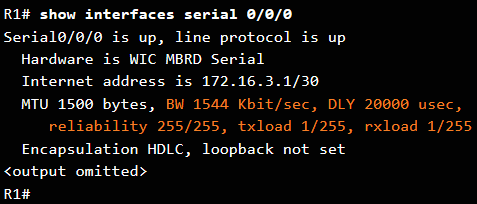
\includegraphics[scale=0.8]{pictures/EIGRPmetric.PNG}
\end{figure}

\begin{itemize}
\item \textbf{BW} -- Bandwidth of the interface (in kilobits per second).
\item \textbf{DLY} -- Delay of the interface (in microseconds).
\item \textbf{Reliability} - Reliability of the interface as a fraction of 255 (255/255 is 100\% reliability), calculated as an exponential average over five minutes. By default, EIGRP does not include its value in computing its metric.
\item \textbf{Txload, Rxload} -- Transmit and receive load on the interface as a fraction of 255 (255/255 is completely saturated), calculated as an exponential average over five minutes. By default, EIGRP does not include its value in computing its metric.
\end{itemize}

\subsubsection{Bandwidth}

EIGRP uses the slowest bandwidth along the path to the destination network. EIGRP divides a reference bandwidth value of $10^7$ by the interface bandwidth value in kb/s. If the result is not a whole number, then the value is rounded down. For example, $10^7$ divided by 1024 equals 9765.625. The .625 is dropped to yield 9765 for the bandwidth portion of the composite metric.

\subsubsection{Delay}

EIGRP uses the sum of all delays along the path to the destination. The sum of these delays is divided by 10. See also table \ref{delay-value} for default delay values.\\

For example, along the path R1$\rightarrow$R2$\rightarrow$R3, the s0/0/1 interface on R2 has a delay of 20,000 microseconds, the g0/0 interface on R3 has a delay of 10 microseconds. The delay is $ \left( 20000 + 10 \right) \div 10 = 2001 $.

\begin{table}[h!]
\centering
\caption{Default delay values}
\label{delay-value}
\begin{tabular}{|l|l|}
\hline
Media            & Delay \\ \hline
Ehternet         & 1000  \\ \hline
Fast Ethernet    & 100   \\ \hline
Gigabit Ethernet & 10    \\ \hline
Serial link      & 20000 \\ \hline
\end{tabular}
\end{table}

\subsection{DUAL algorithm}

EIGRP uses the Diffusing Update Algorithm (DUAL) to provide the best loop-free path and loop-free backup paths. DUAL uses several terms, which are discussed in more detail throughout this section:

\begin{itemize}
\item \textbf{Successor} is a neighboring router that is used for packet forwarding and is the least-cost route to the destination network. The IP address of a successor is shown in a routing table entry right after the word via (see figure \ref{EIGRP-FD}). 

\item \textbf{Feasible Distance (FD)} is the lowest calculated metric to reach the destination network. FD is the metric listed in the routing table entry as the second number inside the brackets (see figure \ref{EIGRP-FD}). As with other routing protocols, this is also known as the metric for the route.

\item \textbf{Feasible Successor (FS)} is a neighbor that has a loop-free backup path to the same network as the successor, and it satisfies the Feasibility Condition (FC). FS is not represented in the routing table until the Successor is down. Instead, we can view FS in topology table (figure \ref{FS}).

\item \textbf{Reported Distance (RD)} is simply an EIGRP neighbor’s FD to the same destination network.

\item \textbf{Feasible Condition (FC)} is met when a neighbor’s RD to a network is less than the local router’s FD to the same destination network. If the RD is less, it represents a loop-free path. 
\end{itemize}

\begin{figure}[hbtp]
\centering
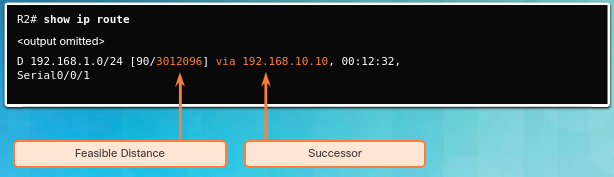
\includegraphics[ width=0.8\textwidth ]{pictures/EIGRP-FD.png}
\caption{Successor and Feasible Distance} \label{EIGRP-FD}
\end{figure}

The decision process for all route computations is done by the DUAL Finite State Machine (FSM). The DUAL FSM tracks all routes and uses EIGRP metrics to select efficient, loop-free paths, and to identify the routes with the least-cost path to be inserted into the routing table.\\

\begin{figure}[hbtp]
\caption{Feasible Successor in Topology table}\label{FS}
\centering
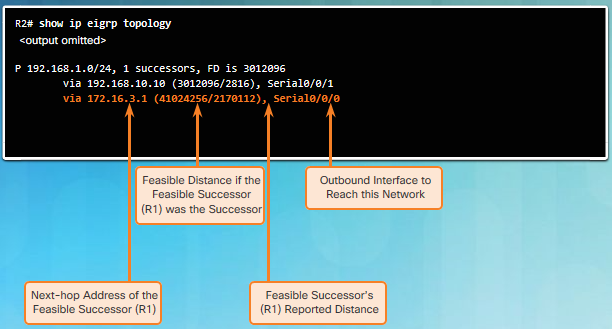
\includegraphics[ width=0.8\textwidth ]{pictures/FS.PNG}
\end{figure}


Recomputation of the DUAL algorithm can be processor-intensive. EIGRP avoids recomputation whenever possible by maintaining a list of backup routes that DUAL has already determined to be loop-free. If the primary route in the routing table fails, the best backup route is immediately added to the routing table.\\

\begin{figure}[hbtp]
\centering
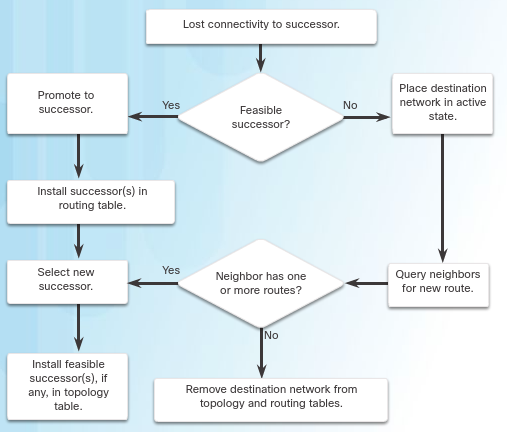
\includegraphics[width=0.7\textwidth]{pictures/EIGRP-DUAL.png}
\caption{DUAL Finite State machine} \label{EIGRP-DUAL}
\end{figure}

When the Successor is no longer available and there is no FS, DUAL puts the route into an \emph{active} state. DUAL sends EIGRP queries asking other routers for a path to the network. Other routers return EIGRP replies, letting the sender of the EIGRP query know whether or not they have a path to the requested network. If none of the EIGRP replies have a path to this network, the sender of the query does not have a route to this network. See also figure \ref{EIGRP-DUAL}.

\subsection{Automatic summarization}

Route summarization allows a router to group networks together and advertises them as one large group using a single, summarized route. Summarization decreases the number of entries in routing updates and lowers the number of entries in local routing tables. It also reduces bandwidth utilization for routing updates and results in faster routing table lookups.\\

However, in classes IP network, the only way that all routers can find the best routes for each individual subnet is for neighbors to send subnet information. In this situation, automatic summarization should be disabled. \\

A problem associated with automatic route summarization is that a summary address also advertises networks that are not available on the advertising router. For example, R1 is advertising the summary address 172.16.0.0/16, but it is only connected to 172.16.1.0/24. Therefore, R1 may receive incoming packets to destinations that do not exist (for example, 172.16.2.0/24). It then forwards a request to a destination network that does not exist, creating a routing loop.\\

EIGRP uses the Null0 interface to avoid the above problem. The Null0 interface is a virtual IOS interface that is a route to nowhere. If R1 receives a packet destined for a network that is advertised by the classful mask but does not exist, it discards the packets by sending them to Null0.\\
 
\note  The Null0 summary route is removed when autosummarization is disabled.

\section{Configuration}

\subsection{EIGRP for IPv4}

\begin{enumerate}
\item Enable EIGRP routing with AS number
	\begin{verbatim}
	R1(config)# router eigrp 10
	\end{verbatim}
	
\item (Optional) Disable auto summarization using \verb|no auto-summary| command.
	
\item Advertise the directly connected networks using the wildcard mask
	\begin{verbatim}
	R1(config-router)# do show ip route | inc C
	R1(config-router)# network 10.1.1.0 0.0.0.3
	R1(config-router)# network 192.168.1.0 0.0.0.255 
	R1(config-router)# network 10.3.3.0 0.0.0.3
	\end{verbatim}
	
\item Configure passive interfaces 
	\begin{verbatim}
	R1(config-router)# passive-interface g0/0
	R1(config-router)# passive-interface g0/1
	\end{verbatim}
	
\item If there are too many passive interfaces, you can make all interfaces of the router to be passive using \verb|passive-interface default|, then configure necessary interface to be active again using \verb|no passive-interface|
	\begin{verbatim}
	R1(config-router)# passive-interface default
	R1(config-router)# no passive-interface s0/0/0
	R1(config-router)# no passive-interface s0/0/1
	\end{verbatim}

\item Examine the EIGRP neighbor table (figure \ref{neigborTable}
	\begin{figure}[hbtp]
	\caption{Examine EIGRP neigbor table}\label{neigborTable}
	\centering
	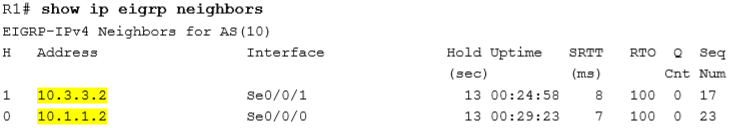
\includegraphics[scale=0.8]{pictures/neigborTable.PNG}
	\end{figure}
	
\item Examine the IP EIGRP routing table using \verb|show ip route eigrp| (figure \ref{EIGRProutingTable})
	\begin{figure}[hbtp]
		\caption{EIGRP routing table}\label{EIGRProutingTable}
		\centering
		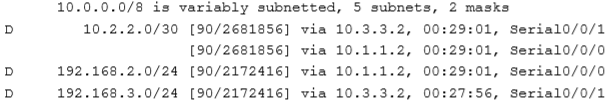
\includegraphics[scale=0.8]{pictures/EIGRProutingTable.PNG}
		\end{figure}

\item Examine the EIGRP topology table using \verb|show ip eigrp topology| (figure \ref{EIGRPtopologyTable})	
	\begin{figure}[hbtp]
			\caption{EIGRP topology table}\label{EIGRPtopologyTable}
			\centering
			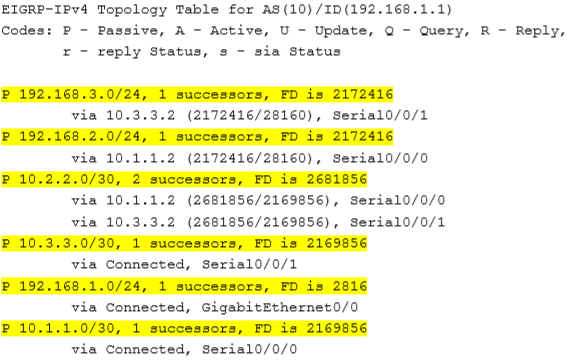
\includegraphics[scale=0.8]{pictures/EIGRPtopologyTable.PNG}
			\end{figure}

\item Verify the EIGRP routing parameters, passive interfaces and networks advertised (figure \ref{EIGRPparameters})
	\begin{figure}[hbtp]
	\caption{EIGRP routing parameters and networks advertised}\label{EIGRPparameters}
	\centering
	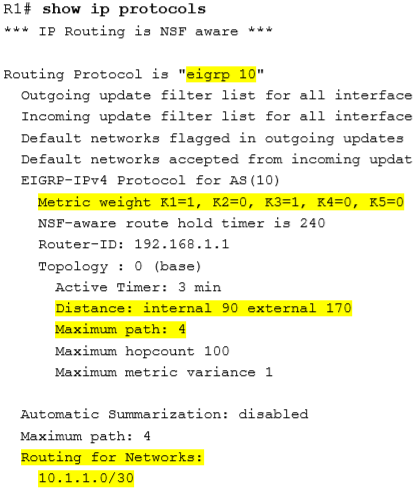
\includegraphics[scale=0.8]{pictures/EIGRPparameters.PNG}
	\end{figure}
						
\end{enumerate}

\subsection{EIGRP for IPv6}

\begin{enumerate}
\item Enable IPv6 routing on the router
	\begin{verbatim}
	R1(config)# ipv6 unicast-routing 
	\end{verbatim}
	
\item Enable EIGRP for IPv6
	\begin{verbatim}
	R1(config)# ipv6 router eigrp 1 
	R1(config-rtr)# no shutdown 
	\end{verbatim}	
	
\item Assign a router ID to each router and 
	\begin{verbatim}
	R1(config)# ipv6 router eigrp 1 
	R1(config-rtr)# eigrp router-id 1.1.1.1
	\end{verbatim}

\item Configure passive interfaces
	\begin{verbatim}
	R1(config)# ipv6 router eigrp 1 
	R1(config-rtr)# passive-interface g0/0 
	\end{verbatim}
	
\item If there are too many passive interfaces, you can make all interfaces of the router to be passive using \verb|passive-interface default|, then configure necessary interface to be active again using \verb|no passive-interface|
	\begin{verbatim}
	R1(config-router)# passive-interface default
	R1(config-router)# no passive-interface s0/0/0
	R1(config-router)# no passive-interface s0/0/1
	\end{verbatim}	
	
\item Configure EIGRP for IPv6 with AS number on each interface
	\begin{verbatim}
	R1(config)# interface g0/0 
	R1(config-if)# ipv6 eigrp 1 
	R1(config-if)# no shutdown
	\end{verbatim}
	
\item Examine the neighbor adjacencies using \verb|show ipv6 eigrp neighbors|
\item Examine the IPv6 EIGRP routing table using \verb|show ipv6 route eigrp|
\item Examine the EIGRP topology using \verb|show ipv6 eigrp topology|
\item Verify the parameters and current state of the active IPv6 routing protocol processes using \verb|show ipv6 protocols|
	
\end{enumerate}
\chapter{OSPF}

\section{Overview}

\subsection{Operation}

\begin{enumerate}
\item \textbf{Establish neighbor adjacencies:} An OSPF-enabled router sends Hello packets out all OSPF-enabled interfaces to determine if neighbors are present on those links.

\item \textbf{Building the Link-State Packets:} Each router builds a link-state packet (LSP) containing the state of \emph{each} directly connected link. 

\item \textbf{Flooding the LSP:} Routers flood their LSPs to all neighbors. To do this, whenever a router receives an LSP from a neighboring router, it immediately sends that LSP out all other interfaces, except the interface that received the LSP. This process creates a flooding effect of LSPs from all routers throughout the routing area.

\item \textbf{Build the Topology Table:} Routers build the topology table (LSDB) based on the received LSPs. 

\item \textbf{Execute the SPF Algorithm:} Routers use the SPF algorithm to create the SPF tree.

\item \textbf{Insert best path to routing table:} From the SPF tree, the best paths are inserted to the IP routing table. The route will remain the routing table unless there is another route with lower administrative distance (AD). Routing decisions are made based on the entries in the routing table, not LSDB.
\end{enumerate}
	
\subsection{OSPF network types}

OSPF defines five network types:

\begin{itemize}
	\item \textbf{Point-to-point} -- Two routers interconnected over a common link. No other routers are on the link. (Figure \ref{point-to-point})
	\item \textbf{Multiaccess} -- Multiple routers interconnected over a switch. (Figure \ref{multiaccess})
	\item \textbf{Nonbroadcast multiaccess (NBMA)} -- Multiple routers interconnected in a network that does not allow broadcasts, such as Frame Relay. (Figure \ref{NBMA})
	\item \textbf{Point-to-multipoint} -- Multiple routers interconnected in a hub-and-spoke topology over an NBMA network (Figure \ref{point-to-multipoin}).
	\item \textbf{Virtual links} -- Special OSPF network used to interconnect distant OSPF areas to the backbone area (Figure \ref{virtual-link}). In this scenario, area 51 cannot connect directly to area 0. A special OSPF area must be configured to connect area 51 to area 0. The R1 and R2 in area 1 must be configured as a virtual link.
\end{itemize}
	
\begin{figure}%
	\centering
	\subfigure[Point-to-point]{\includegraphics[width=0.4\textwidth]{point-to-point.png} \label{point-to-point}}
	\subfigure[Multiaccess]{\includegraphics[width=0.4\textwidth]{multiaccess.png} \label{multiaccess}}
	\subfigure[Nonbroadcast multiaccess]{\includegraphics[width=0.4\textwidth]{pictures/NBMA.png} \label{NBMA}}
	\subfigure[Point-to-multipoint]{\includegraphics[width=0.4\textwidth]{pictures/point-to-multipoint.png} \label{point-to-multipoin}}
	\subfigure[Virtual link]{\includegraphics[width=0.4\textwidth]{pictures/virtual-link.png} \label{virtual-link}}
	\caption{OSPF network types}
	\label{network-types}
	\end{figure}
	
\subsection{OSPF cost}

OSPF uses \textbf{cost} as a metric, where lower cost indicates a better path. The cost of an interface is inversely proportional to the bandwidth of the interface:
\[ \text{cost}=\frac{\text{Reference bandwidth}}{\text{Interface bandwidth}} \]
The default reference bandwidth is 100 Mb/s, therefore the formula is:
\[ \text{cost}=\frac{10^8}{\text{Interface bandwidth in bps}} \]
Notice that any interfaces faster than 100 Mb/s share the same cost 1, because the OSPF cost value must be an integer. To avoid this, changing reference bandwidth to a higher value than 100 Mb/s is required. \\

\note Changing the reference bandwidth does not actually affect the physical bandwidth of the device; rather, it simply affects the calculation used to determine the metric.

\section{Protocol components}
The OSPF routing protocol has three main components:
\begin{itemize}
	\item Data structures
	\item Routing protocol messages
	\item Algorithm
	\end{itemize}
	
\subsection{Data structure}

Data structures are the tables or databases that OSPF builds in order to operate. OSPF creates and maintains three databases. These databases are kept and maintained in RAM.

\begin{itemize}
	\item \textbf{Adjacency database} (neighbor table) is a list of all neighbor routers, and unique for each router. It can be viewed using \texttt{show ip ospf neigbor} command.
	\item \textbf{Link-state database or LSDB} (topology table) shows the network topology and is identical for all routers in one area. It can be viewed using \texttt{show ip ospf database} command.
	\item \textbf{Forwarding database} (Routing table) is a list of best routes to reach networks. In the routing table, OSPF intra-area routes start with O, inter-area routes start with O IA, external routes start with O E1 (or O E2).
\end{itemize}

\subsection{Messages}

OSPF messages are transmitted to multicast address 01-00-5E-00-00-0\textbf{5} and 01-00-5E-00-00-0\textbf{6} in MAC address, 224.0.0.5 and 224.0.0.4 in IPv4, or FF02::5 and FF02::6 in IPv6. The protocol field in IP packet header is set to \textbf{89} for OSPF protocol.\\

OSPF uses five types of packets to convey routing information:
\begin{itemize}
	\item \textbf{Hello packets} establish neighbor adjacency, and facilitate the DR, BDR election in multiaccess network.
	\item \textbf{Database description (DBD) packets} contain an abbreviated LSDB.
	\item \textbf{Link-State Request (LSR) packets} request additional information about network.
	\item \textbf{Link-State Update (LSU) packets} are sent only to neighbors \emph{every 30 minutes}, or as a response to LSRs, or when a change is perceived.
	\item \textbf{Link-State Acknowledgment (LSAck) packets} are used to confirm receipt of the LSU.
\end{itemize}

\subsubsection{Hello and dead intervals}

The frequency at which the router sends hello packets is specified by hello interval in packet header. The default hello interval on point-to-point and multiaccess network is 10 seconds, on NBMA is 30 seconds.\\

Another important timer is dead interval, which is the period that the router waits to receive a hello packet before declaring the neighbor down. By default, dead interval is \emph{four times hello interval}.

\subsubsection{Link-State Advertisement}

The link-state advertisement (LSA) is a basic communication means of the OSPF routing protocol. It describes a building block of the LSDB. Individually, they act as database records and provide specific OSPF network details.\\
 
LSAs are not LSPs, they are actually packaged inside LSPs to convey different kinds of routing information. The use of terms LSU, LSP and LSA can sometimes confusing because these terms are often used interchangeably. However, they are different: \emph{An LSU is a type of LSP, an LSP contains one or more LSAs}.\\
 
LSA has its own header, which includes link-state type, link's cost, sequence number, the address of advertising router, and link ID. The \emph{link ID} field identifies the piece of the routing domain based on LSA type (see table \ref{LSA-type}).

\begin{table}[h]
\centering
\caption{Link-State Advertisment types}
\label{LSA-type}
\begin{tabular}{ | p{2em} | p{3em} | p{0.4\textwidth} | p{0.2\textwidth} | p{0.2\textwidth} | }
\hline
LSA type & Sending router & Description                                            & Flooding area        & Link ID                             \\ \hline
1        & all routers    & Introduce directly connected networks to its neighbors & one area             & router ID of the originating router \\ \hline
2        & DR             & Give other routers info about multiaccess network      & one area             & IP interface address of DR		\\ \hline
3        & ABR            & Propagates info of each area to all other routers      & between areas        & network address                 \\ \hline
4        & ABR            & Identify ASBR and provide the route to it              & entire routing domain& router ID of ASBR                 \\ \hline
5        & ASBR, ABR      & Advertise external network                             & entire routing domain& external network address         \\ \hline
\end{tabular}
\end{table}

Receiving a type 3 LSA does not cause a router to run the SPF algorithm, but the routes being advertised in the type 3 LSAs are appropriately updated to the routing table.

\subsection{Algorithm}\label{sec:algorithm}

When an OSPF router is initially connected to a network, it goes through the following states in order:
\begin{enumerate}
\item \textbf{Down state} (send hello packets but cannot receive them)
\item \textbf{Init state} (send and receive hello packets)
\item \textbf{Two-way state} (elect a DR and a BDR)
\item \textbf{ExStart state} (decide which router will send the DBD packets first, the router with higher router ID will be the first one to send DBD packets)%negotiate the master/slave relationship and DBD packet sequence number
\item \textbf{Exchange state} (exchange DBD packets)
\item \textbf{Loading state} (if the information in DBD packets is different from the LSDB, a router will transition to this state to gain additional route information, using LSRs)
\item \textbf{Full state} (reach convergence)
\end{enumerate}

SPF algorithm calculates the best paths in order: calculate intra-area routes $\rightarrow$ calculate inter-area routes $\rightarrow$ calculate external routes.

\section{DR election}

\subsection{Terminologies}

\paragraph{Multiaccess network} can create challenges for the flooding of LSPs. Ethernet network interconnects routers over a common link, therefore each router considers all counterparts in multiaccess network are its neighbors and establish adjacency to each of them (see figure \ref{multiple-adjacencies}). This could lead to extensive flooding of LSPs when OSPF is initialized or when topology changes.

\begin{figure}[hbtp]
\centering
\includegraphics[width=0.7\textwidth]{multiple-adjacencies.png} 
\caption{Creating adjacencies with every neighbors in multiaccess network}
\label{multiple-adjacencies}
\end{figure}
	
\paragraph{Designated Router (DR)} is the solution to the problems on multiaccess network. On multiaccess networks and multiaccess networks only, OSPF elects a DR to be the collection and distribution point for LSPs sent and received. The router with the  The router ID of DR can be viewed using \texttt{show ip ospf interface} command on any routers within the multiaccess network.
	
\paragraph{Backup Designated Router (BDR)} is also elected. The BDR listens passively to this exchange and maintains a relationship with all the routers. If the DR stops producing Hello packets, the BDR promotes itself and assumes the role of DR.
	
\paragraph{DROTHERs} are all other routers that are neither the DR nor the BDR. Each DROTHER forms full adjacencies (Full state) with the DR and BDR and form 2-way adjacencies (Two-way state) with any DROTHERs (see figure \ref{DR-adjacency}). DROTHERs only send their LSPs to the DR and BDR using the multicast address \textbf{224.0.0.6} (DR-routers address). All DROTHER routers still receive Hello packets from each other.
	
\begin{figure}[hbtp]
\centering
\includegraphics[width=0.4\textwidth]{pictures/dr-bdr.jpeg}
\caption{DROTHERs only form full adjacencies with the DR and BDR in the network}
\label{DR-adjacency}
\end{figure}

\emph{Every router requires a router ID to participate in an OSPF domain.} The router ID is used by the OSPF-enabled router to Uniquely identify the router and Participate in DR election. Cisco routers derive the router ID in one of three ways and with the following precedence: 

\begin{enumerate}
\item Router ID configured with the OSPF router-id command, if present 
\item Highest IP address of any of the router’s loopback addresses, if present 
\item Highest active IP address on any of the router’s physical interfaces
\end{enumerate}

\subsection{Election decision}
	
The OSPF DR and BDR election decision is based on the following criteria, in sequential order:

\begin{enumerate}
\item The routers in the network elect the router with the highest interface priority as the DR. The router with the second highest interface priority is elected as the BDR.
\item If the interface priorities are equal, then the router with the highest router ID is elected the DR. The router with the second highest router ID is the BDR.
\end{enumerate}
	
After the DR is elected, it remains the DR until one of the following events occurs:

\begin{itemize}
\item The DR fails
\item The OSPF process on the DR fails or is stopped
\item The multiaccess interface on the DR fails or is shutdown
\end{itemize}
	
The DR and BDR elections are not pre-emptive. If a new router with a higher priority or higher router ID is added to the network after the DR and BDR election, the newly added router does not take over the DR or the BDR role. This is because those roles have already been assigned. The addition of a new router does not initiate a new election process.\\

If the DR fails, the BDR is automatically promoted to DR. This is the case even if a new router with a higher priority or router ID is added to the network after the initial DR/BDR election. However, after a BDR is promoted to DR, a new BDR election occurs and the new router is elected as BDR.

\section{OSPF area}
An OSPF area is a group of routers that share the same link-state information in their LSDBs. An instance of OSPF can have several areas (called Multi-area OSPF). Implementing multiple OSPF areas has many advantages:

\begin{itemize}
\item Smaller routing table (There are fewer routing table entries as network addresses can be summarized between areas.)
\item Reduced link-state update overhead (Fewer routers exchanging LSAs because LSA flooding stops at the area boundary.)
\item Reduced frequency of SPF calculations (Routing still occurs between the areas, however, the CPU intensive routing operation of recalculating the SPF algorithm is done only for routes within an area.)
\end{itemize}

To make multi-area OSPF more efficient and scalable, a two-layer area hierarchy is implemented:

\begin{itemize}
\item \textbf{Backbone (Transit) area} -- A backbone area directly connected with all other areas. All traffic moving from one area to another area must traverse the backbone area. Generally, end users are not found within a backbone area. The backbone area is always OSPF area 0.
\item \textbf{Regular (Non-backbone) area} -- Connects users and resources. By default, a regular area does not allow traffic from another area to use its links to reach other areas. All traffic from other areas must cross a transit area.
\end{itemize}

In multi-area OSPF, there are four different types of OSPF routers:

\begin{itemize}
\item Internal router (have all interfaces in the same area)
\item Backbone router (reside in backbone area)
\item Area border router or ABR (have interfaces attached to multiple areas)
\item Autonomous System Boundary Router or ASBR (have at least one interface attached to an external network)
\end{itemize}

\section{Configuration}

\subsection{Recommendations}

The optimal number of routers per area varies based on factors such as network stability, but Cisco recommends the following guidelines:
\begin{itemize}
\item An area should have no more than 50 routers.
\item A router should not be in more than three areas.
\item Any single router should not have more than 60 neighbors.
\end{itemize}

Also keep the following notes in mind:
\begin{itemize}
\item Propagating type 3 and 5 LSAs can cause significant flooding problems. For this reason, it is strongly recommended that manual route summarization be configured on the ABRs and ASBR.
\item For routers to become adjacent, their Hello interval, Dead interval, area ID (not process ID), subnet masks, and Stub area flag must match.
\item  The dead interval must be larger than Hello interval.
\end{itemize}

\subsection{OSPF for IPv4}

\begin{enumerate}
\item Enable OSPF routing with process ID
	\begin{verbatim}
	R1(config)# router ospf 1
	\end{verbatim}
	
\item Configure the network statements for directly connected network
	\begin{verbatim}
	R1(config-router)# network 192.168.1.0 0.0.0.255 area 0 
	R1(config-router)# network 192.168.12.0 0.0.0.3 area 1 
	R1(config-router)# network 192.168.13.0 0.0.0.3 area 2
	\end{verbatim}
	
\item Configure passive interfaces
	\begin{verbatim} 
	R1(config-rtr)# passive-interface g0/0 
	R1(config-rtr)# passive-interface g0/1
	\end{verbatim}	

\item If there are too many passive interfaces, you can make all interfaces of the router to be passive using \verb|passive-interface default|, then configure necessary interface to be active again using \verb|no passive-interface|
	\begin{verbatim}
	R1(config-router)# passive-interface default
	R1(config-router)# no passive-interface s0/0/0
	R1(config-router)# no passive-interface s0/0/1
	\end{verbatim}		
	
\item Propagating a default static route. \note Do not use \verb|redistribute static| as this command will not recognize default static route (due to auto summarization, it only recognizes classful route).
	\begin{verbatim}
	R1(config)# router ospf 1
	R1(config-router)# default-information originate
	\end{verbatim}
	
\item Verify configuration using the following commands:
	\begin{itemize}
	\item \verb|show ip protocols|
	\item \verb|show ip ospf neighbor|
	\item \verb|show ip route ospf|
	\item \verb|show ip ospf|
	\item \verb|show ip ospf interface brief|
	\end{itemize}		
\end{enumerate}

\subsection{OSPF for IPv6}

\begin{enumerate}
\item Enable IPv6 routing on the router
	\begin{verbatim}
	R1(config)# ipv6 unicast-routing 
	\end{verbatim}
	
\item Enable OSPF for IPv6
	\begin{verbatim}
	R1(config)# ipv6 router ospf 1 
	R1(config-rtr)# no shutdown 
	\end{verbatim}	
	
\item Assign a router ID to each router
	\begin{verbatim}
	R1(config)# ipv6 router ospf 1 
	R1(config-rtr)# router-id 1.1.1.1
	\end{verbatim}

\item Configure passive interfaces
	\begin{verbatim}
	R1(config)# ipv6 router ospf 1 
	R1(config-rtr)# passive-interface g0/0 
	\end{verbatim}
	
\item If there are too many passive interfaces, you can make all interfaces of the router to be passive using \verb|passive-interface default|, then configure necessary interface to be active again using \verb|no passive-interface|
	\begin{verbatim}
	R1(config-router)# passive-interface default
	R1(config-router)# no passive-interface s0/0/0
	R1(config-router)# no passive-interface s0/0/1
	\end{verbatim}	
	
\item Configure OSPF for IPv6 with area number on each interface
	\begin{verbatim}
	R1(config)# interface g0/0 
	R1(config-if)# ipv6 ospf 1 area 0
	R1(config-if)# no shutdown
	R1(config-if)# interface g0/1       
	R1(config-if)# ipv6 ospf 1 area 55
	R1(config-if)# no shutdown
	\end{verbatim}     
	
\end{enumerate}	

\subsection{Summarization}

The following command enables Inter-area route summarization (for ABRs only). It summarizes all routes in an area to the specified summary address.

\begin{verbatim}
R1(config)# router ospf 1
R1(config-router)# area 1 range 192.168.64.0 255.255.224.0
\end{verbatim}

The following command enables External route summarization (for ASBRs only). It advertises a single route for all redistributed routes that are covered by a specified network.

\begin{verbatim}
R1(config)# router ospf 1
R1(config-router)# summary-address 192.168.64.0 255.255.224.0
\end{verbatim}

\subsection{Priority}

Configure OSPF priority for each interface. The higher the priority value (from 0 to 255), the more likely the router becomes the DR or BDR on the interface.	The priority of 0 means that the router will never  become a DR or BDR. On the other hand, 255 means the router will always be DR or BDR. As for IPv6, replace \verb|ip| by \verb|ipv6|.
	\begin{verbatim}
	R1(config)# interface g0/0 
	R1(config)# ip ospf priority 150
	\end{verbatim}
	
\subsection{Dead and Hello interval}

Configure OSPF Dead interval, Hello interval (in seconds). \note The Dead interval must not be smaller than the Hello interval. By default, the Dead interval is four times the Hello interval. As for IPv6, replace \verb|ip| by \verb|ipv6|.
	\begin{verbatim}
	R1(config)# interface g0/0
	R1(config-if)# ip ospf hello-interval 20 
	R1(config-if)# ip ospf dead-interval 80
	\end{verbatim}
	
\subsection{Reference bandwidth}	

Change reference bandwidth to 1000 Mb/s.
	\begin{verbatim}
	R1(config)# interface g0/0
	R1(config-if)# auto-cost reference-bandwidth 1000
	\end{verbatim}
	
\subsection{Assign OSPF cost}	

Directly assign OSPF cost. The cost is a number between 1 and 65,535. As for IPv6, replace \verb|ip| by \verb|ipv6|.
	\begin{verbatim}
	R1(config)# interface g0/0
	R1(config-if)# ip ospf cost 1564
	\end{verbatim}

\subsection{Verification}
Examine the neighbor adjacencies using \verb|show ip ospf neighbors|, routing table using \verb|show ip route ospf|, topology using \verb|show ip ospf interface|. Verify the parameters and current state of OSPF processes using \verb|show ipv6 protocols|.	As for IPv6, replace \verb|ip| by \verb|ipv6|.

\part{WAN TECHNOLOGIES}
\chapter{PPP}

\section{Introduction}

HDLC is the default serial encapsulation method when connecting two Cisco routers and it can only work with other Cisco devices. HDLC is now the basis for \emph{synchronous} point-to-point used by many servers to connect to a WAN, most commonly the Internet. However, when there is a need to connect to a non-Cisco router, PPP encapsulation should be used.\\

There are many advantages to using PPP, including the fact that it is not proprietary. PPP provides router-to-router and host-to-network connections over \emph{synchronous} and \emph{asynchronous} circuits. PPP includes many features not available in HDLC: The link quality management feature (LQM) monitors the quality of the link, PAP and CHAP authentication.\\

\begin{figure}[hbtp]
\caption{PPP layered architecture}\label{PPPlayers}
\centering
\includegraphics[ width=0.8\textwidth ]{pictures/PPPlayers.PNG}
\end{figure}

PPP contains three main components: HDLC-like framing, LCP, and NCPs. \\

Figure \ref{PPPlayers} maps the layered architecture of PPP against the OSI model. PPP and OSI share the same physical layer, but PPP distributes the functions of LCP and NCP differently. Most of the work done by PPP happens at the data link and network layers, by LCP and NCPs.

\section{Operation}

\subsection{Frame Structure}

A PPP frame consists of six fields. The following descriptions summarize the PPP frame fields illustrated in the figure \ref{PPPframe}: 

\begin{figure}[hbtp]
\caption{PPP Frame fields}\label{PPPframe}
\centering
\includegraphics[ width=0.8\textwidth ]{pictures/PPPframe.PNG}
\end{figure}


\begin{itemize}
\item \textbf{Flag:}  A single byte that indicates the beginning or end of a frame. The Flag field consists of the binary sequence 01111110 (63 in decimal). 


\item \textbf{Address:}   A single byte that contains the broadcast address because PPP does not assign individual station addresses. 


\item \textbf{Control:}   A single byte that contains the binary sequence 00000011, which calls for transmission of user data in an unsequenced frame. 

\item \textbf{Protocol:}   Two bytes that identify the protocol encapsulated in the information field of the frame. The 2-byte Protocol field identifies the protocol of the PPP payload.  

\item \textbf{Frame Check Sequence (FCS):} This is 2 bytes. If the receiver’s calculation of the FCS does not match the FCS in the PPP frame, the PPP frame is silently discarded.
\end{itemize}

\subsection{Establishing a PPP Session}

There are three phases of establishing a PPP session:

\begin{itemize}
\item \textbf{Phase 1: Link establishment and configuration negotiation} -- The LCP opens the connection and negotiates configuration options. This phase is complete when the receiving router sends a configuration-acknowledgment frame back to the router initiating the connection. 


\item \textbf{Phase 2: Link quality determination (optional)} -- The LCP tests the link to determine whether the link quality is sufficient to bring up network layer protocols. The LCP can delay transmission of network layer protocol information until this phase is complete. 


\item \textbf{Phase 3: Network layer protocol configuration negotiation} -- After the LCP has finished the link quality determination phase, the appropriate NCP can separately configure the network layer protocols. If the LCP closes the link, it informs NCPs so that they can take appropriate action.
\end{itemize}

\subsection{LCP}

Link Control Protocol (LCP) operation uses three classes of LCP frames to accomplish the work of each of the LCP phases: Link-establishment $\rightarrow$ Link-maintenance $\rightarrow$ Link-termination (Figure \ref{PPPEstablishment}).

\begin{figure}[hbtp]
\caption{Establish PPP session: Link-establishment, Link-maintenance, Link-termination}\label{PPPEstablishment}
\centering
\includegraphics[ width=0.6\textwidth ]{pictures/PPPEstablishment.PNG}
\end{figure}


\subsubsection{Link Establishment}

The link establishment process starts with the initiating device sending a Configure-Request frame to the responder. The initiator includes the options for how it wants the link created, including protocol or authentication parameters. The responder processes the request: 

\begin{itemize}
\item If the options are not acceptable or not recognized, the responder sends a Configure-Nak or Configure-Reject message. If this occurs and the negotiation fails, the initiator must restart the process with new options. 


\item If the options are acceptable, the responder responds with a Configure-Ack message and the process moves on to the authentication stage. The operation of the link is handed over to the NCP.
\end{itemize}

\subsubsection{Link Maintenance}

When NCP has completed all necessary configurations, LCP transitions into link maintenance. During link maintenance, LCP can use messages to provide feedback and test the link using:

\begin{itemize}
\item Echo-Request, Echo-Reply, and Discard-Request: These frames can be used for testing the link.


\item Code-Reject and Protocol-Reject: These frame types provide feedback when one device receives an invalid frame. The sending device will resend the packet.
\end{itemize} 

\subsubsection{Link termination}

After the transfer of data at the network layer completes, the LCP terminates the link, as shown in Figure \ref{PPPEstablishment}. NCP only terminates the network layer and NCP link. The link remains open until the LCP terminates it. If the LCP terminates the link before NCP, the NCP session is also terminated. \\

The LCP closes the link by exchanging Terminate packets. The device initiating the shutdown sends a Terminate-Request message. The other device replies with a Terminate-Ack. 

\subsection{NCP}

After the LCP has configured and authenticated the basic link, the appropriate NCP is invoked to complete the specific configuration of the network layer protocol being used.\\

IPCP is an example of NCP. IPCP is responsible for configuring, enabling, and disabling the IPv4 modules on both ends of the link. IPCP negotiates two options:

\begin{itemize}
\item \textbf{Compression:} Allows devices to negotiate an algorithm to compress TCP and IP headers and save bandwidth.

\item \textbf{IPv4-Address:} Allows the initiating device to specify an IPv4 address to use for routing IP over the PPP link, or to request an IPv4 address for the responder.
\end{itemize}

\subsection{Authentication}

\paragraph{PAP}is a very basic \textbf{two-way handshake}. There is no encryption. The username and password are sent in plaintext. If it is accepted, the connection is allowed. CHAP is more secure than PAP. PAP may be used in the following environments: CHAP is not supported, or simulate a login at the remote host. 

\paragraph{PAP Process}\emph{After link establishment phase}, the remote node sends a username-password pair in plain text across the link. At the receiving node, the username-password is checked. This device either allows or denies the connection. An accept or reject message is returned to the requester.

\paragraph{CHAP}Unlike PAP, which only authenticates once, CHAP uses a \textbf{three-way handshake}, and conducts periodic challenges to make sure that the remote node still has a valid password value. The password value is variable and changes unpredictably while the link exists. Thus, CHAP provides protection against a playback attack.

\paragraph{CHAP process}\emph{After link establishment phase}, the local router sends a challenge message to the remote node. The remote node responds with a value that is calculated using a one-way hash function. The local router checks the response against its own calculation. If the values match, the initiating node acknowledges the authentication. If the values do not match, the initiating node immediately terminates the connection.

\section{Configuration}

\paragraph{Basic:} To set PPP as the encapsulation method used by a serial interface, use the encapsulation ppp interface configuration command.
	\begin{verbatim}
	interface s0/0/0
		encapsulation ppp
		no shutdown
	\end{verbatim}
	
\paragraph{Compression:} Point-to-point software compression on serial interfaces can be configured after PPP encapsulation is enabled. If the traffic already consists of compressed files, such as .zip, .tar, or .mpeg, do not use this option.
	\begin{verbatim}
	compress [predictor | stac]	
	\end{verbatim}
	
\paragraph{Quality check:} The \verb|ppp quality 80| command ensures that the link meets the quality requirement set (80\%); otherwise, the link closes down.

\paragraph{Multilink PPP:} provides a method for spreading traffic across multiple physical WAN links. allows packets to be fragmented and sends these fragments simultaneously over multiple point-to-point links to the same remote address. 
	\begin{verbatim}
	interface s0/0/0
		no ip address
		encapsulation ppp
		ppp multilink	
		ppp multilink group 1
		no shutdown
		
	interface s0/0/1
		no ip address
		encapsulation ppp
		ppp multilink	
		ppp multilink group 1
		no shutdown
		
	interface Multilink 1
		ip address 10.0.1.1 255.255.255.252
		ppp multilink	
		ppp multilink group 1			
	\end{verbatim}
	
\paragraph{CHAP Authentication:} The hostname (e.g. R3, R2, ISP) on one router must match the username the other router has configured in the command \verb|username <name> password <password>| . The passwords must also match.
	\begin{verbatim}
	Router(config)# hostname ISP
	ISP(config)# username R3 secret cisco
	ISP(config)# interface s0/0/0
	ISP(config-if)# ppp authentication chap
	
	Router(config)# hostname R3
	R3(config)# username ISP secret cisco
	R3(config)# interface serial0/1/0
	R3(config-if)# ppp authentication chap	
	\end{verbatim}
	
\paragraph{PAP Authentication:} The PAP username and password are configured in the command \verb|ppp pap sent-username|. Theses username and password must match those specified with the \verb|username <name> password <password>| command on the other router.
	\begin{verbatim}
	R1(config)# username R3 secret class
	R1(config)# interface s0/0/0
	R1(config-if)# ppp authentication pap
	R1(config-if)# ppp pap sent-username R1 password cisco
	
	R3(config)# username R1 secret cisco
	R3(config)# interface s0/0/0
	R3(config-if)# ppp authentication pap
	R3(config-if)# ppp pap sent-username R3 password class	
	
	username R3 secret class
	ppp pap sent-username R3 password class
	
	username R1 secret cisco
	ppp pap sent-username R1 password cisco
	\end{verbatim}
\chapter{PPPoE, GRE, eBGP}

\section{PPPoE}

Ethernet links do not natively support PPP. A solution to this problem is PPP over Ethernet (PPPoE). PPPoE creates a PPP tunnel over an Ethernet connection. This allows PPP frames to be sent across the Ethernet cable to the ISP from the customer’s router.\\

To create a PPP tunnel, the configuration uses a \emph{dialer interface}. A dialer interface is a virtual interface. The PPP configuration is placed on the dialer interface, not the physical interface. The PPP CHAP is then configured with hostname Cust1 and password cisco123. Then, dialer interface is linked to the Ethernet interface with the \verb|dialer pool| command. Remember to set MTU to 1492 to accommodate PPPoE headers. The physical Ethernet interface g0/1 with PPPoE is enabled with the command \verb|pppoe enable| interface configuration command. Then it is linked to the Dialer interface with the \verb|pppoe-client dial-pool-number <number>| interface configuration command.


\begin{sexylisting}{PPPoE}
interface dialer 1
  encapsulation ppp
  ip address negotiated
interface dialer 1
  ppp authentication chap callin
  ppp chap host name Cust1
  ppp chap password cisco123  
interface dialer 1
  dialer pool 1
  mtu 1492
  no shutdown  
interface g0/1
  no ip address
  pppoe enable
  pppoe-client dial-pool-number 1
end

show ip int brief
show int dialer 1
show ip route
show pppoe session
debug ppp {negotiation | authentication | events}  
\end{sexylisting}

\section{GRE}

\subsection{Introduction}

GRE, IPsec, web-based SSL are the three methods of establishing a VPN connection offered by Cisco devices. GRE is a out-dated, non-secure, stateless, site-to-site VPN tunneling protocol. GRE supports the encapsulation of \textbf{any OSI Layer 3 protocol} and \textbf{47} is used in the protocol field in IP header (figure \ref{GREpacket}). GRE also supports multiprotocol and IP multicast tunneling.\\

GRE is the default tunnel interface mode for Cisco IOS software. GRE does not provide encryption or any other security mechanisms. Therefore, data that is sent across a GRE tunnel is not secure.\\

\begin{figure}[hbtp]
\caption{Header for GRE encapsulated packet header}\label{GREpacket}
\centering
\includegraphics[scale=1]{pictures/GREpacket.PNG}
\end{figure}

Three circumstances can cause a GRE tunnel to be in an up/down state:
\begin{itemize}
\item The tunnel interface is down.
\item A valid route to the destination address is missing from the routing table.
\item The tunnel address is routed through the tunnel itself.
\end{itemize}

\subsection{Configuration}

Five steps to configuring a GRE tunnel (figure \ref{GREexample}):

\begin{figure}[hbtp]
\caption{Configure GRE VPN tunnel}\label{GREexample}
\centering
\includegraphics[scale=0.5]{pictures/GREexample.PNG}
\end{figure}

\begin{enumerate}
\item \textbf{Create a tunnel interface:} \\

Configure the tunnel interface on the WEST router. Use s0/0/0 as the tunnel source interface and 10.2.2.1 (IP address of EAST router s0/0/1) as the tunnel destination.

\begin{verbatim}
WEST(config)# interface tunnel 0
WEST(config-if)# ip address 172.16.12.1 255.255.255.252
WEST(config-if)# tunnel source s0/0/0
WEST(config-if)# tunnel destination 10.2.2.1
\end{verbatim}

Configure the tunnel interface on the EAST router. Use s0/0/1 as the tunnel source interface and 10.1.1.1 (IP address of WEST router s0/0/0) as the tunnel destination.

\begin{verbatim}
EAST(config)# interface tunnel 0
EAST(config-if)# ip address 172.16.12.2 255.255.255.252
EAST(config-if)# tunnel source 10.2.2.1
EAST(config-if)# tunnel destination 10.1.1.1
\end{verbatim}

\item \textbf{Verify that the GRE tunnel is functional:} Verify the status of the tunnel interface on the WEST and EAST routers using \verb|show interface tunnel 0| and \verb|show ip interface brief| commands.

\item \textbf{Enable routing over the GRE Tunnel:} After the GRE tunnel is set up, the routing protocol can be implemented. For GRE tunneling, a network statement will include the \underline{IP network of the tunnel}, instead of the network associated with the serial interface. Remember that the ISP router is not participating in this routing process.

\begin{verbatim}
WEST(config)# router ospf 1
WEST(config-router)# network 172.16.12.0 0.0.0.3 area 0

EAST(config)# router ospf 1
EAST(config-router)# network 172.16.12.0 0.0.0.3 area 0
\end{verbatim}

If BGP is used instead of OSPF or EIGRP, the neighbor statement will include the \underline{IP network of the tunnel}, instead of the network associated with the serial interface.

\begin{verbatim}
WEST(config)# router bgp 65000 
WEST(config-router)# neighbor 172.16.12.2 remote-as 65001

EAST(config)# router bgp 65001
EAST(config-router)# neighbor 172.16.12.1 remote-as 65000
\end{verbatim}

\end{enumerate}

\section{eBGP}

\subsection{Introduction}

Border Gateway Protocol (BGP) is an Exterior Gateway Protocol (EGP). BGP updates are encapsulated over TCP on port \textbf{179}. We use BGP when an autonomous system (AS) has connections to \emph{multiple} ASs (known as multi-homed). BGP should not be used when there is a \emph{single} connection to the Internet or another AS (known as single-homed).\\

There are three common ways an organization can choose to implement BGP in a multi-homed environment: Default Route Only, Default Route and ISP Routes, All Internet Routes (this would include routes to over 550,000 networks).\\

External BGP is the routing protocol used between routers in different autonomous systems. Internal BGP is the routing protocol used between routers in the same AS. Two routers exchanging BGP routing information are known as BGP peers.\\

Internal routing protocols (OSPF, EIGRP, RIP, etc.) use a specific metric (e.g. OSPF’s cost) for determining the best paths to destination networks. BGP does \emph{not} use a \emph{single} metric like IGPs. Instead it uses several \emph{attributes} including a list of AS numbers necessary to reach a destination network. Therefore BGP is known as a \emph{path vector} routing protocol. Also, because of this, a misconfiguration of a BGP router could have negative effects throughout the entire Internet.

\subsection{Configuration}

To implement eBGP for this course, you will need to complete the following tasks:
\begin{enumerate}
\item Enable BGP routing and identify the AS number
\item Configure BGP neighbor(s) (peering).
\item Advertise network(s) originating from this AS.
\end{enumerate}

\begin{verbatim}
R2(config)# router bgp 65000 
R2(config-router)# neighbor 209.165.200.1 remote-as 65001
R2(config-router)# network 198.133.219.0 mask 255.255.255.248 
R2(config-router)# end
R2# show ip route
R2# show ip bgp 
R2# show ip bgp summary
\end{verbatim}


\chapter{Quality of Service}

\section{Introduction}

\subsection{Traffic characteristics}

\paragraph{Voice}Voice traffic is predictable and smooth. However, voice is delay-sensitive and there is no reason to re-transmit voice if packets are lost. Therefore, voice packets must receive a higher priority than other types of traffic. Latency should be no more than \textbf{150 ms}. Jitter should be no more than \textbf{30 ms}, and voice packet loss should be no more than \textbf{1\%}. Voice traffic requires at least \textbf{30 Kbps} of bandwidth.

\paragraph{Video}Video traffic tends to be unpredictable, inconsistent, and bursty compared to voice traffic. Compared to voice, video is less resilient to loss and has a higher volume of data per packet. Latency should be no more than \textbf{400 ms}. Jitter should be no more than \textbf{50 ms}, and video packet loss should be no more than \textbf{1\%}. Video traffic requires at least \textbf{384 Kbps} of bandwidth.

\paragraph{Data}Data traffic is relatively insensitive to drops and delays compared to voice and video. The two main factors a network administrator needs to ask about the flow of data traffic are the following: Does the data come from an interactive application? Is the data mission critical?

\paragraph{Delay} Network congestion causes delay. Two types of delays are fixed and variable. A fixed delay is a specific amount of time a specific process takes, such as how long it takes to place a bit on the transmission media. A variable delay take an unspecified amount of time and is affected by factors such as how much traffic is being processed. \emph{Jitter} is the variation in the delay of received packets.

\subsection{QoS tools}

When the volume of traffic is greater than what can be transported across the network, network devices (router, switch, etc.) hold the packets in memory until resources become available to transmit them. If the number of packets continues to increase, the memory within the device fills up and packets are dropped. This problem can be solved by either increasing link capacity or implementing QoS.\\

A device implements QoS only when it is experiencing congestion. There are three categories of QoS tools: Classification and marking, Congestion avoidance, Congestion management. Refer to Figure \ref{QoStools} to help understand the sequence of how these tools are used when QoS is applied to packet flows.\\

\begin{figure}[hbtp]
\caption{QoS sequence}\label{QoStools}
\centering
\includegraphics[ width=0.8\textwidth ]{pictures/QoStools.PNG}
\end{figure}

\section{Congestion management}
When traffic exceeds available network resources, Congestion management buffers and prioritizes packets before being transmitted to the destination. Common Cisco IOS-based congestion management tools include CBWFQ and LLQ algorithms.

\subsection{WFQ}

WFQ (Weighted Fair Queuing) is an automated scheduling method that provides fair bandwidth allocation to all network traffic. \\

WFQ applies priority to identified traffic and classifies it into flows, as shown in the figure \ref{WFQ}. WFQ then determines how much bandwidth each flow is allowed. WFQ classifies traffic into different flows based on packet header addressing.\\

\begin{figure}[hbtp]
\caption{WFQ example}\label{WFQ}
\centering
\includegraphics[ width=0.8\textwidth ]{pictures/WFQ.PNG}
\end{figure}

WFQ is not supported with tunneling and encryption. It does not allow users to take control over bandwidth allocation.

\subsection{CBWFQ}

Class-Based Weighted Fair Queuing (CBWFQ) extends the standard WFQ functionality to provide support for user-defined traffic classes. For CBWFQ, you define traffic classes based on match criteria including protocols, access control lists (ACLs), and input interfaces.\\

To characterize a class, you assign it bandwidth, weight, and queue limit. After a queue has reached its configured queue limit, adding more packets to the class causes tail drop. Tail drop means a router simply discards any packet that arrives at the end of a queue.

\subsection{LLQ}

The Low Latency Queuing (LLQ) feature brings strict priority queuing to CBWFQ. Strict PQ allows voice to be sent first. Without LLQ, CBWFQ services fairly based on weight; no class of packets may be granted strict priority. This scheme poses problems for voice traffic that is largely intolerant of delay.

\section{QoS models}
The three models for implementing QoS are: Best-effort model, Integrated services (IntServ), Differentiated services (DiffServ). Best-effort model means \emph{no QoS} is implemented. QoS is really implemented in a network using either IntServ or DiffServ.

\subsection{Best effort}

The best-effort model (meaning no QoS) treats all network packets in the same way. This model is used when QoS is not required. The table \ref{BestEffort} lists the benefits and drawbacks of the best effort model. 

\begin{table}[hbtp]
\centering
\caption{Pros and Cons of Best-effort}\label{BestEffort}
\begin{tabular}{ll}
\toprule
\head{Benefits} & \head{Drawbacks} \\ 
\midrule 
Most scalable & No guarantees of delivery \\  
Scalability is limited by bandwidth & Packets can arrive in any order \\ 
No special QoS mechanism required & No packets have preferential treatment \\ 
Easy to deploy & Critical data is treated the same as casual one \\ 
\bottomrule
\end{tabular}
\end{table} 

\subsection{Integrated services}

Integrated Services (IntServ) is a multiple-service model that can accommodate multiple QoS requirements.\\

It uses resource reservation and admission-control mechanisms as building blocks to establish and maintain QoS. Each individual communication must explicitly specify its traffic descriptor and requested resources to the network (Figure \ref{IntServ}). The edge router performs admission control to ensure that available resources are sufficient in the network.\\

\begin{figure}[hbtp]
\caption{Simple IntServ example}\label{IntServ}
\centering
\includegraphics[scale=0.7]{pictures/IntServ.PNG}
\end{figure}

IntServ uses the Resource Reservation Protocol (RSVP) to signal the QoS needs of an application’s traffic along devices in the end-to-end path through the network. If network devices along the path can reserve the necessary bandwidth, the originating application can begin transmitting. If the requested reservation fails along the path, the originating application does not send any data.\\

\begin{table}[hbtp]
\centering
\caption{Pros and Cons of IntServ}
\begin{tabular}{ll}
\toprule
\head{Benefits} & \head{Drawbacks} \\ 
\midrule 
Explicit end-to-end resource admission control & Resource intensive \\  
Per-request policy admission control & Not scalable \\ 
Signaling of dynamic port numbers &  \\ 
\bottomrule
\end{tabular}
\end{table} 

\subsection{Differentiated services}

The DiffServ design overcomes the limitations of both the best-effort and IntServ models. Unlike IntServ, DiffServ is not an end-to-end QoS strategy and does not use signaling. Instead, DiffServ uses a “soft QoS” approach (Figure \ref{DiffServ1}). For example, DiffServ can provide low-latency guaranteed service to voice or video while providing best-effort traffic to web traffic or file transfers.\\

\begin{figure}[hbtp]
\caption{Simple DiffServ example}\label{DiffServ1}
\centering
\includegraphics[scale=0.7]{pictures/DiffServ.PNG}
\end{figure}


Specifically, DiffServ divides network traffic into classes based on business requirements. Each of the classes can then be assigned a different level of service. You pay for a level of service. Throughout the network, the level of service you paid for is recognized and your package is given either preferential or normal traffic, depending on what you requested.\\

\begin{table}[hbtp]
\centering
\caption{Pros and Cons of DiffServ}\label{DiffServ2}
\begin{tabular}{ll}
\toprule
\head{Benefits} & \head{Drawbacks} \\ 
\midrule 
Highly scalable & No absolute guarantee of delivery \\  
Many different levels of quality & Requires complex mechanisms \\ 
\bottomrule
\end{tabular}
\end{table} 

\section{Classification and marking}

Before a packet can have a QoS policy applied to it, the packet has to be classified. Classification and marking identifies types of packets. Traffic should be classified and marked as close to its source as technically and administratively feasible. This defines the trust boundary. \\

Marking means that we are adding a value to the packet header. Devices receiving the packet look at this field to see if it matches a defined policy.\\

Trusted endpoints have the capabilities and intelligence to mark application traffic to the appropriate Layer 2 CoS and/or Layer 3 DSCP values. Examples of trusted endpoints include IP phones, wireless access points, videoconferencing gateways and systems, IP conferencing stations, and more.\\

Methods of classifying traffic flows at Layer 2 and 3 include using interfaces, ACLs, and class maps.

\subsection{Marking at Layer 2}

802.1Q is the IEEE standard that supports VLAN tagging at layer 2 on Ethernet networks. The 802.1Q standard also includes the QoS prioritization scheme known as IEEE 802.1p. The 802.1p standard uses the first three bits in the Tag Control Information (TCI) field (Figure \ref{CoS}). Known as the Priority (PRI) field, this 3-bit field identifies the Class of Service (CoS) markings.\\

\begin{figure}[hbtp]
\caption{Ethernet Class of Service values}\label{CoS}
\centering
\includegraphics[ width=0.8\textwidth ]{pictures/CoS.PNG}
\end{figure}

\subsection{Marking at Layer 3}

The benefit of deploying Layer 3 marking is that it can carry QoS information end-to-end unlike Layer 2 marking, which changes frame header as well as QoS information hop by hop.\\

Both IPv4 and IPv6 support an 8-bit field for marking, the Type of Service (ToS) field for IPv4 and the Traffic Class field for IPv6. Figure \ref{ToS} displays the contents of the 8-bit field. The field has 6-bits allocated for QoS, called the \textbf{DiffServ} Code Point (DSCP) field. The remaining two IP Extended Congestion Notification (ECN) bits can be used by ECN-aware routers to mark packets instead of dropping them. The ECN marking informs downstream routers that there is congestion in the packet flow. \\

\begin{figure}[hbtp]
\caption{Type of Service/Traffic Class Field}\label{ToS}
\centering
\includegraphics[ width=0.8\textwidth ]{pictures/ToS.PNG}
\end{figure}

The DSCP values are organized into three categories: 
\begin{itemize}
\item \textbf{Best-Effort (BE):} When a router experiences congestion, these packets will be dropped. No QoS plan is implemented.
\item \textbf{Expedited Forwarding (EF):} DSCP decimal value is 46 (binary 101110). At Layer 3, Cisco recommends that EF only be used to mark voice packets.
\item \textbf{Assured Forwarding (AF):} Use the 5 most significant DSCP bits to indicate queues and drop preference. As shown in Figure \ref{DSCP}, the first 3 most significant bits are used to designate the class. The 4th and 5th most significant bits are used to designate the drop preference. The 6th most significant bit is set to zero. The AFxy formula shows how the AF values are calculated. For example, AF32 belongs to class 3 (binary 011) and has a medium drop preference (binary 10).
\end{itemize}

\begin{figure}[hbtp]
\caption{Assured forwarding values}\label{DSCP}
\centering
\includegraphics[ scale=0.7 ]{pictures/DSCP.PNG}
\end{figure}

\section{Congestion Avoidance}

We avoid congestion by dropping lower-priority packets before congestion occurs. When the queue fills up to the maximum threshold, a small percentage of packets are dropped. When the maximum threshold is passed, all packets are dropped. WRED, traffic shaping, and traffic policing are three mechanisms provided by Cisco IOS QoS software to prevent congestion. 

\paragraph{WRED} is the primary congestion avoidance tool. It regulates TCP data traffic before tail drops (caused by queue overflows) occur.

\paragraph{Traffic shaping}retains excess packets in a queue and then schedules the excess for later transmission over increments of time. The result of traffic shaping is a smoothed packet output rate, as shown in Figure \ref{Spacing}. Ensure that you have sufficient memory when enabling shaping.\\

\begin{figure}[hbtp]
\caption{Spacing traffic example}\label{Spacing}
\centering
\includegraphics[scale=0.7]{pictures/Spacing.PNG}
\end{figure}

\paragraph{Traffic policing}Shaping is an outbound concept; packets going out an interface get queued and can be shaped. In contrast, policing is applied to inbound traffic on an interface. When the traffic rate reaches the configured maximum rate, excess traffic is dropped (or remarked), as shown in figure \ref{policing}.\\

\begin{figure}[hbtp]
\caption{Spacing traffic example}\label{policing}
\centering
\includegraphics[ scale=0.7 ]{pictures/policing.PNG}
\end{figure}

\part{INFRASTRUCTURE SERVICE}
\chapter{DHCPv4}

\section{Operation}

DHCPv4 works in a client/server mode. When a client communicates with a DHCPv4 server, the server assigns or leases an IPv4 address to that client. The client connects to the network with that leased IP address until the lease expires.\\

The client must contact the DHCP server periodically to extend the lease. This lease mechanism ensures that clients that move or power off do not keep addresses that they no longer need. When a lease expires, the DHCP server returns the address to the pool where it can be reallocated as necessary.\\

\subsection{Lease origination}

When the client boots (or otherwise wants to join a network), it begins DORA\footnote{DORA = Discovery, Offer, Request, Acknowledgement} process to obtain a lease.

\begin{enumerate}
\item A client starts the process with a broadcast \textbf{DHCP-DISCOVER} message to finds available DHCPv4 servers.

\item When the DHCPv4 server receives a DHCP-DISCOVER message, it reserves an available IPv4 address to lease to the client. It then sends a \textbf{DHCP-OFFER} message to the requesting client. The server also creates an ARP entry consisting of the MAC address of the requesting client and the leased IPv4 address of the client.

\item When the client receives the DHCP-OFFER from the server, it broadcasts\textbf{DHCP-REQUEST} messages. The DHCP-REQUEST serves as an acceptance notice to the selected server and an implicit decline to any other servers.

\item On receiving the DHCP-REQUEST message, the server verifies the lease information with an ICMP ping to that address to ensure it is not being used already. If there is \emph{no} ICMP echo reply, then the address is is not being used by any client. Otherwise, that address is being used and the server has to send DHCP-OFFER again.

\item DHCP server sends  unicast \textbf{DHCP-ACK} message to the client. The DHCP-ACK message informs the client that the IP address is valid. Because The DHCP-ACK message is a duplicate of the DHCP-OFFER, it also provides IP information for the client.

\item When the client receives the DHCPACK message, performs an ARP lookup for the assigned address.
If there is no reply to the ARP, the client knows that the IPv4 address is valid and starts using it as its own.
\end{enumerate}



\subsection{Lease renewal}

\begin{enumerate}
\item Before the lease expires, the client sends a DHCPREQUEST message directly to DHCPv4 server. If a DHCPACK is not received within a specified amount of time, the client broadcasts another DHCPREQUEST so that one of the other DHCPv4 servers can extend the lease.

\item On receiving the DHCPREQUEST message, the server verifies the lease information by returning a DHCPACK
\end{enumerate}

\subsection{Relay agent}

Sometimes, network clients are not on the same subnet as DHCP servers. Because routers do not forward broadcasts, the DHCP-REQUEST from clients are not sent to DHCP server.\\

Cisco offers a solution called Cisco IOS helper address. This solution enables a router to forward DHCP-REQUEST broadcasts to the DHCPv4 server. When
a router forwards address assignment/parameter requests, it is acting as a DHCPv4 \emph{relay agent}.

\section{Message}

DHCPv4 messages UDP encapsulation. The server uses port 67, the client uses port 68.

\subsection{Message format}

\paragraph{Operation (OP) code}specifies general type of message: request (1), reply (2).

\begin{figure}[hbtp]
\caption{DHCPv4 message format}
\centering
\includegraphics[ width=0.8\textwidth ]{pictures/DHCPmessage.PNG}
\end{figure}

\paragraph{Hardware type} Ethernet (1), Frame Relay (15), Serial (20)

\paragraph{Hop}Controls the forwarding of messages. Set to 0 by a client before transmitting a request.

\paragraph{Transaction identifier} used by client to match the request with replies from DHCPv4 server.

\paragraph{Seconds} amount of time (in seconds) elapsed since a client attempted to acquire or renew a lease.

\paragraph{Flag}Used by a client that does not know its IPv4 address when it sends a
request. Only one of the 16 bits—the broadcast flag—is used. A value of 1 in
this field tells the DHCPv4 server or relay agent receiving the request that the
reply should be sent as a broadcast.

\subsection{DHCP-DISCOVER}

When the client boots, it has no way of knowing the subnet to which it belongs. Therefore, destination
IPv4 address of DCHP-DISCOVER is 255.255.255.255, the destination MAC address is FF:FF:FF:FF:FF:FF. The source MAC address is the MAC address of the client. The client does not have a configured IPv4 address
yet, so the source IPv4 address is 0.0.0.0 

\subsection{DHCP-OFFER}

DHCP-OFFER contains initial configuration information
for the client: IPv4 address for client, subnet mask, lease duration, and IPv4 address of the DHCPv4 server. The DHCPOFFER message can be configured to include other information, such as the lease renewal time and DNS address.


\section{Configuration}

\subsection{DHCPv4 server}

\begin{description}
\item[Step 1.] \textbf{Exclude addresses:} Some IPv4 addresses in a pool are assigned to network devices that require static address assignments. Therefore, these IPv4 addresses should not be assigned to other devices.

\begin{verbatim}
R1(config)# ip dhcp excluded-address <ip-address>
R1(config)# ip dhcp excluded-address 192.168.10.1

R1(config)# ip dhcp excluded-address <range-of-address>
R1(config)# ip dhcp excluded-address 192.168.10.1 192.168.10.9
\end{verbatim}

\item[Step 2.] \textbf{Configure address pool:} Define a pool of addresses to assign to clients.

\begin{verbatim}
R1(config)# ip dhcp pool <pool-name>
R1(dhcp-config)# network <network-range>

R1(config)# ip dhcp pool LAN-POOL-1
R1(dhcp-config)# network 192.168.10.0 255.255.255.0
\end{verbatim}

\item[Step 3.] Define the default gateway router for clients. 

\begin{verbatim}
R1(dhcp-config)# default-router 192.168.10.1
\end{verbatim}

\item[Step 4.] \textbf{Relay agent:} If network clients are not on the same subnet as DHCP servers, configure the default gateway as a relay agent.

\begin{verbatim}
R1(config)# interface g0/0
R1(config-if)# ip helper-address 192.168.11.6
\end{verbatim}

\item[Step 4 (Optional)] Other DHCP specifics

\begin{verbatim}
R1(dhcp-config)# dns-server 192.168.11.5
R1(dhcp-config)# domain-name example.com
\end{verbatim}

\item[Step 5. Verification] The \verb|show ip dhcp binding| command displays a list of all IPv4 address to MACaddress bindings that have been provided by the DHCPv4 service. The \verb|show ip dhcp server statistics| command verifies that messages are being received or sent by the router. This command displays count information regarding the number of DHCPv4 messages that have been sent and received.

\begin{verbatim}
R1# show run | sec dhcp
R1# show ip dhcp binding
R1# show ip dhcp statistics
\end{verbatim}
\end{description}

\subsection{DHCPv4 client}

\begin{verbatim}
SOHO(config)# interface g0/1
SOHO(config-if)# ip address dhcp
SOHO(config-if)# no shutdown
\end{verbatim}


\chapter{DHCPv6}

\section{General Operation}

When the client boots up, it sends DHCPv6 SOLICIT message to FF02::1:2, which is the multicast all-DHCPv6-server address. One or more servers respond with a DHCPv6 ADVERTISE unicast message to inform the client that the server is available for DHCPv6 service. The client responds with either a DHCPv6 REQUEST or a DHCPv6 INFORMATION-REQUEST unicast message: 

\begin{itemize}
\item DHCPv6 INFORMATION-REQUEST unicast message is used for Stateless DHCPv6 (i.e. SLAAC, Stateless DHCPv6 and SLAAC) to request only additional information, such as DNS server addresses, domain name.
\item DHCPv6 REQUEST unicast message is used for Stateful DHCPv6 to ask for IP configuration parameters from the server.
\end{itemize}

The server sends a DHCPv6 REPLY unicast message to the client containing the information requested in the DHCPv6 REQUEST or DHCPv6 INFORMATION REQUEST message.

\section{SLAAC}

Stateless Address AutoConfiguration (SLAAC) is enabled by default. Both the M flag and the O flag are set to 0 in the RA. In SLAAC, a host automatically obtains its IP configuration from an IPv6-enabled router. The host generates its own unique IPv6 address. A DHCPv6 server is not required. SLAAC operation includes the following steps:

\begin{enumerate}
\item Client asks for IPv6 configuration by sending an RS to the router R1.
\item R1 receives the RS message and responds with an RA message.
\item PC1 receives the RA, and uses the information in the message to create its own IPv6 global unicast address. 
\item Because SLAAC is a stateless process, PC1 must verify that this newly created IPv6 address is unique using DAD process.
\end{enumerate}

\begin{figure}[hbtp]
\caption{Verify SLAAC method}
\centering
\includegraphics[scale=0.8]{pictures/SLAAC.PNG}
\end{figure}


To configure SLAAC, use the \verb|no ipv6 nd managed-config-flag| and \verb|ipv6 nd other-config-flag| in router interface configuration mode.

\section{SLAAC and Stateless DHCPv6}

A host obtains IP configuration (prefix, prefix-length, default gateway) using SLAAC and additional information (DNS server, domain name, etc.) from a stateless DHCPv6 server. The host generates its own unique IPv6 address. \\

There are four steps to configure a router as a DHCPv6 server:

\begin{enumerate}
\item Enable IPv6 Routing using \verb|ipv6 unicast-routing| command
\item Use \verb|ipv6 dhcp pool <pool-name>| command to create a pool and enter the router in DHCPv6 configuration mode
\item (Optional) In DHCPv6 configuration mode, configure DNS server address (\verb|dns-server <ip-address>|) and domain name (\verb|domain-name <name>|).
\item In the interface configuration mode, we bind the DHCPv6 pool to the interface using \verb|ipv6 dhcp server <pool-name>|
\item For stateless DHCPv6, the O flag is 1 and the M flag is 0, therefore, to indicate stateless DHCPv6, use the \verb|ipv6 nd other-config-flag| in router interface configuration mode.
\end{enumerate}

\begin{figure}[hbtp]
\caption{Verify Stateless DHCPv6 method}
\centering
\includegraphics[scale=0.8]{pictures/Stateless-DHCPv6.PNG}
\end{figure}


\begin{verbatim}
R1(config)# ipv6 unicast-routing
R1(config)#
R1(config)# ipv6 dhcp pool IPV6-STATELESS
R1(config-dhcpv6)# dns-server 2001:db8:cafe:aaaa::5
R1(config-dhcpv6)# domain-name example.com
R1(config-dhcpv6)# exit
R1(config)#
R1(config)# interface g0/1
R1(config-if)# ipv6 address 2001:db8:cafe:1::1/64
R1(config-if)# ipv6 dhcp server IPV6-STATELESS
R1(config-if)# ipv6 nd other-config-flag
R1(config-if)# end
R1# show ipv6 dhcp pool 
R1# show ipv6 interface
R1# debug ipv6 dhcp detail
\end{verbatim}

The \verb|show ipv6 dhcp pool| command verifies the name of the DHCPv6 pool and its parameters. The \verb|show ipv6 interface| command  confirms that the interface has ``Stateless address autoconfig enabled'' and has an IPv6 global unicast address. 

\section{Stateful DHCPv6}

In stateful DHCPv6, all IP information information must be obtained from a stateful DHCPv6 server. However, the default router information is not from the DHCPv6 server, but
it was determined by using the source IPv6 address from the RA message. This is known as \emph{stateful} DHCPv6 because the DHCPv6 server maintains IPv6 state information.\\

DHCPv6 messages from the server to the client use \textbf{UDP} destination port \textbf{546}. The client sends DHCPv6 messages to the server using \textbf{UDP} destination port \textbf{547}.\\

There are four steps to configure a router as a DHCPv6 server:

\begin{enumerate}
\item Enable IPv6 Routing using \verb|ipv6 unicast-routing| command
\item Use \verb|ipv6 dhcp pool <pool-name>| command to create a pool and enter the router in DHCPv6 configuration mode
\item In DHCPv6 configuration mode, \verb|address prefix <prefix/length> lifetime <time> <preferred-time>|. The \verb|lifetime| option indicates the valid and preferred lease times in seconds.
\item (Optional) Configure DNS server address (\verb|dns-server <ip-address>|) and domain name (\verb|domain-name <name>|).
\item In the interface configuration mode, we bind the DHCPv6 pool to the interface using \verb|ipv6 dhcp server <pool-name>|
\item Because the M flag indicates whether or not to use stateful DHCPv6 and the O flag is not involved, to signify stateful DHCPv6, we set the M flag as 1 using \verb|ipv6 nd managed-config-flag| in router interface configuration mode.
\end{enumerate}

\begin{figure}[hbtp]
\caption{Verify stateful DHCPv6}
\centering
\includegraphics[scale=0.8]{pictures/Stateful-DHCPv6.PNG}
\end{figure}


\begin{verbatim}
R1(config)# ipv6 unicast-routing
R1(config)#
R1(config)# ipv6 dhcp pool IPV6-STATEFUL
R1(config-dhcpv6)# address prefix 2001:DB8:CAFE:1::/64 lifetime infinite infinite
R1(config-dhcpv6)# dns-server 2001:db8:cafe:aaaa::5
R1(config-dhcpv6)# domain-name example.com
R1(config-dhcpv6)# exit
R1(config)#
R1(config)# interface g0/1
R1(config-if)# ipv6 address 2001:db8:cafe:1::1/64
R1(config-if)# ipv6 dhcp server IPV6-STATEFUL
R1(config-if)# ipv6 nd managed-config-flag
R1(config-if)# end
\end{verbatim}

The \verb|show ipv6 dhcp pool| command verifies the name of the DHCPv6 pool and its parameters. The \verb|show ipv6 dhcp binding| command in Example 8-22 displays the automatic
binding between the link-local address of the client and the address that the server assigns. 

\section{Router as DHCPv6 client}

In the following commands, a Cisco router is used as the stateless DHCPv6 client. The \verb|ipv6 enable| command is used because the router does not yet have a global unicast address. The \verb|ipv6 address autoconfig| command enables automatic configuration of IPv6 addressing using SLAAC. By assumption, the server router is configured for stateless DHCPv6, so it sends an RA message to inform the client router to use stateless DHCPv6 to obtain DNS information.

\begin{verbatim}
R3(config)# interface g0/1
R3(config-if)# ipv6 enable
R3(config-if)# ipv6 address autoconfig
R3(config-if)# end
\end{verbatim}

\section{Relay agent}

If the DHCPv6 server is located on a different network than the client, the IPv6 router can be configured as a DHCPv6 relay agent using \verb|ipv6 dhcp relay destination 2001:db8:cafe:1::6| command in interface configuration mode.

\section{Message}

\paragraph{Router solicitation (RS)} The client sends an RS message to the router. The destination address of the message is \textbf{all-routers} multicast address \textbf{FF02::2}.

\paragraph{Router advertisement (RA)} is sent by routers to provide IP configuration to clients. The RA message includes IPv6 configuration for clients (prefix, prefix-length, DNS server, MTU, and default gateway information). A router sends an RA message periodically (every 200s) or in response to an RS message. RA messages are always sent to the IPv6 \textbf{all-nodes} multicast address \textbf{FF02::1}.\\

The two flags are the Managed Address Configuration flag (M flag) and the Other Configuration flag (O flag). Using different combinations of the M and O flags, RA messages have one of three addressing options for the IPv6 device:

\begin{itemize}
\item SLAAC (M = 0, O = 0)
\item SLAAC and Stateless DHCPv6 (M = 0, O = 1)
\item Stateful DHCPv6 (M = 1)
\end{itemize}



\chapter{HSRP}

\section{Operations}

One way to prevent a single point of failure at the default gateway, is to implement a virtual router. To implement this type of router redundancy, multiple routers are configured by First Hop Redundancy Protocol (FHRP) to work together as an illusion of a single router to the hosts on the LAN. One the most popular options for FHRP is Hot Standby Router Protocol (HSRP). HSRP was designed by Cisco to allow for gateway redundancy without any additional configuration on end devices.\\
 
One of the routers is selected by HSRP to be the active router. The active router will act as the default gateway for end devices. The other router will become the standby router. The default gateway address is a virtual IPv4 address along with a virtual MAC address that is shared amongst both HSRP routers. End devices use this virtual IPv4 address as their default gateway address.(See figure \ref{HSRP-topology}). The virtual IPv4 address is configured by the network administrator. The virtual MAC address is created automatically.

\begin{figure}[hbtp]
\centering
\includegraphics[width=0.6\textwidth]{pictures/HSRP.png}
\caption{HSRP topology}
\label{HSRP-topology}
\end{figure}

\section{Priority}

HSRP priority can be used to determine the active router. The router with the highest HSRP priority will become the active router. By default, the HSRP priority is 100. If the priorities are equal, the router with the numerically highest IPv4 address is elected as the active router.

\section{Preemption}

By default, after a router becomes the active router, it will remain the active router even if another router comes online with a higher HSRP priority. This means that the router which boots up first will become the active router if there are no other routers online during the election process.\\

To force a new HSRP election process, preemption must be enabled. Preemption is the ability of an HSRP router to trigger the re-election process. With preemption enabled, a router that comes online with a higher HSRP priority will assume the role of the active router. Preemption only allows a router to become the active router if it has a higher priority. However, a router with equal priority will not preempt an active router, even if it has higher IPv4 address.

\section{States and timers}

When an interface is configured with HSRP, it exchanges HSRP hello packets to determine which router is active. Hello packets are sent to the HSRP group multicast address every 3 seconds (hello timer), by default. The standby router will become active if it does not receive a hello message from the active router after 10 seconds (hold timer). To avoid increased CPU usage and unnecessary standby state changes, do not set the hello timer below 1 second or the hold timer below 4 seconds.

\section{Configuration}
Complete the following steps to configure HSRP (see figure \ref{HSRP-config} for example):
\begin{enumerate}
    \item Configure HSRP version 2.
    \item Configure the virtual IP address for the group.
    \item Configure the priority for the desired active router to be greater than 100.
    \item Configure the active router to preempt the standby router in cases where the active router comes online after the standby router.
    \end{enumerate}
\begin{verbatim}
R1(config)# interface g0/1
R1(config-if)# ip address 172.16.10.2 255.255.255.0
R1(config-if)# standby version 2
R1(config-if)# standby 1 ip 172.16.10.1
R1(config-if)# standby 1 priority 150
R1(config-if)# standby 1 preempt
R1(config-if)# no shutdown
\end{verbatim}


\part{INFRASTRUCTURE SECURITY}
\chapter{NAT}

\section{What is NAT?}

NAT provides the translation of private addresses to public addresses. Its primary use is to conserve public IPv4 addresses. A NAT router typically operates at the border of a stub network\footnote{A stub network is a network that has a single connection to its neighboring network -- one way in and one way out of the network.} (Figure \ref{NATborder}). Table \ref{ProsAndCons} shows the advantages and disadvantages of NAT.\\

\begin{figure}[hbtp]
\caption{NAT border}\label{NATborder}
\centering
\includegraphics[ width=0.7\textwidth ]{pictures/NATborder.PNG}
\end{figure}

\begin{table}[hbtp]
\centering\caption{Pros and Cons of NAT}\label{ProsAndCons}
\begin{tabular}{ p{7cm} p{7cm} }
\toprule
\head{Advantages} & \head{Disadvantages} \\

Conserves the legally registered addressing scheme by allowing the privatization of intranets &
End-to-end functionality is degraded\footnote{NAT increases forwarding delays because the translation of each IPv4 address within the packet headers takes time.} \\

Increases the flexibility of connections to the public network &
End-to-end IP traceability is lost \\

Provides consistency for internal network addressing schemes\footnote{NAT allows the existing private IPv4 address scheme to remain while allowing for easy change to a new public addressing scheme. This means an organization could change ISPs and not need to change any of its inside clients.} & 
Tunneling becomes more complicated \\
\bottomrule
\end{tabular}
\end{table}

In NAT terminology, the inside network is the set of networks that is subject to translation. The outside network refers to all other networks. NAT includes four types of addresses:

\begin{figure}[hbtp]
\caption{Types of NAT addresses}
\centering
\includegraphics[ width=0.7\textwidth ]{pictures/NATterm.PNG}
\end{figure}


\begin{itemize}
\item \textbf{Inside address:} The address of the device that NAT is translating.
\item \textbf{Outside address:} The address of the destination device.
\item \textbf{Local address:} A local address is any address that appears on the inside portion of the network.
\item \textbf{Global address:} A global address is any address that appears on the outside portion of the network.
\end{itemize}

There are three types of NAT translation: static NAT, dynamic NAT, PAT (Port address translation).

\section{Operation}

In Figure \ref{NAToperation}, PC1 with private address 192.168.10.10 wants to communicate with an outside web server with public address 209.165.201.1.

\begin{figure}[hbtp]
\caption{NAT in action}\label{NAToperation}
\centering
\includegraphics[ width=0.6\textwidth ]{pictures/NAToperation.PNG}
\end{figure}

When the packet arrives at R2 (NAT-enabled router), R2 reads the source IPv4 address of the packet to determine if the packet matches the criteria specified for translation. In this case, the source IPv4 address does match the criteria and is translated from 192.168.10.10 (inside local address) to 209.165.200.226 (inside global address). R2 adds this mapping of the local to global address to the NAT table. R2 sends the packet with the translated source address toward the destination.\\

The web server responds with a packet addressed to the inside global address of PC1 (209.165.200.226). R2 receives the packet with destination address 209.165.200.226. R2 checks the NAT table and finds an entry for this mapping. R2 uses this information and translates the inside global address (209.165.200.226) to the inside local address (192.168.10.10), and the packet is forwarded toward PC1.

\section{Static NAT}

Static NAT is \textbf{one-to-one} address mapping between local and global addresses. Static NAT is particularly useful for servers or devices that must have a consistent address. There are three basic steps when configuring static NAT translations:

\begin{enumerate}
\item Create a mapping between the inside local address and the inside global addresses using the \verb|ip nat inside | \verb|source static <local-ip> <global-ip>| in global configuration.

\item The interfaces participating in the translation are configured as inside or outside relative to NAT. Inside interfaces are configured with the \verb|ip nat inside| interface configuration command, whereas the outside interface is configured with the \verb|ip nat outside| interface configuration command.

\item Verify NAT configuration using \verb|show ip nat translations| or \verb|show ip nat statistics|.
\end{enumerate}

\begin{verbatim}
R2(config)# ip nat inside source static 192.168.10.254 209.165.201.5
R2(config)#
R2(config)# interface Serial0/0/0
R2(config-if)# ip nat inside
R2(config-if)# interface Serial0/1/0
R2(config-if)# ip nat outside
R2(config-if)# end
\end{verbatim}

\section{Dynamic NAT}

Dynamic NAT is \textbf{many-to-many} address mapping between local and global addresses. If there are 100 inside local addresses and 10 inside global addresses, at any given time only 10 of the 100 inside local addresses can be translated. Dynamic NAT uses a pool of public addresses and assigns them on a first-come, firstserved basis. There are six steps when configuring dynamic NAT translations:

\begin{enumerate}
\item Define the pool of addresses to be used for translation. The pool is assigned a name to identify it. Use \verb|ip nat pool | \verb|<pool-name> <start-ip> <end-ip>| \verb|netmask <netmask>|.

\item Configure a standard ACL

\item Bind the ACL to the pool. Use the \verb|ip nat inside | \verb|source list | \verb|<ACL-name>| \verb|pool| \verb|<pool-name>| global configuration.

\item The interfaces participating in the translation are configured as inside or outside relative to NAT. Inside interfaces are configured with the \verb|ip nat inside| interface configuration command, whereas the outside interface is configured with the \verb|ip nat outside| interface configuration command.

\item Verify NAT configuration using \verb|show ip nat translations| or \verb|show ip nat statistics|.
\end{enumerate}

\begin{verbatim}
R2(config)# ip nat pool NAT-POOL1 209.165.200.226 209.165.200.240 netmask 255.255.255.224
R2(config)#
R2(config)# access-list 1 permit 192.168.0.0 0.0.255.255
R2(config)#
R2(config)# ip nat inside source list 1 pool NAT-POOL1
R2(config)#
R2(config)# interface Serial0/0/0
R2(config-if)# ip nat inside
R2(config-if)# exit
R2(config)#
R2(config)# interface Serial0/1/0
R2(config-if)# ip nat outside
R2(config-if)#
\end{verbatim}

\section{PAT}

PAT (also known as NAT overloading) is a \textbf{many-to-one} address mapping between local and global addresses. With PAT, multiple addresses can be mapped to one or to a few addresses because each private address is also tracked by a port number. For example, if there are 100 inside local addresses and 10 inside global addresses, PAT uses ports as an additional parameter to provide a multiplier effect, making it possible to reuse any one of the 10 inside global addresses.\\

When the NAT router receives a packet from the client, it uses its source port number to uniquely identify the specific NAT translation. PAT ensures that devices use a different TCP port number for each session with a server on the Internet. When a response comes back from the server, the source port number, which becomes the destination port number on the return trip, determines to which device the router forwards the packets. \\

\begin{figure}[hbtp]
\caption{PAT in action}\label{PAT}
\centering
\includegraphics[ width=0.6\textwidth]{pictures/PAT.PNG}
\end{figure}

\begin{table}[hbtp]
\centering \caption{PAT table of Figure \ref{PAT} }
\begin{tabular}{ll | l}
\toprule
\head{Inside local} & \head{Inside global} & \head{Outside global} \\
\midrule
192.168.10.10:1555 & 209.165.200.226:1555 & 209.165.201.1:80 \\
192.168.10.11:1331 & 209.165.200.226:1331 & 209.165.202.129:80 \\
\bottomrule
\end{tabular}
\end{table}

In Figure \ref{PAT}, R2 uses port numbers (1331 and 1555) to identify the device from which the packet originated. In this example, the service port is 80, which is HTTP. For the source address, R2 translates the inside local address to an inside global address with the port number added. Note that, the client port numbers, 1331 and 1555, did not change at the NAT-enabled router. The destination address is the outside global IPv4 address of servers. \\

When there are no more ports available and there is more than one external address in the address pool, PAT moves to the next address to try to allocate the original source port. This process continues until there are no more available ports or external IPv4 addresses.\\

PAT also translates some protocols that do not use TCP or UDP. Each of these types of protocols is handled differently by PAT. For example, ICMPv4 query messages, echo requests, and echo replies include a Query ID. ICMPv4 uses the Query ID to identify an echo request with its corresponding echo reply. \\

There are six steps when configuring dynamic PAT translations. The six steps are identical to configuring dynamic NAT except for step 3.

\begin{enumerate}
\item Define the pool of addresses to be used for translation. The pool is assigned a name to identify it. Use \verb|ip nat pool | \verb|<pool-name> <start-ip> <end-ip>| \verb|netmask <netmask>|.

\item Configure a standard ACL

\item Bind the ACL to the pool. Use the \verb|ip nat inside | \verb|source list | \verb|<ACL-name>| \verb|pool| \verb|<pool-name>| \verb|overload| in global configuration mode. The \verb|overload| keyword is the primary difference between PAT and dynamic NAT.

\item The interfaces participating in the translation are configured as inside or outside relative to NAT. Inside interfaces are configured with the \verb|ip nat inside| interface configuration command, whereas the outside interface is configured with the \verb|ip nat outside| interface configuration command.

\item Verify NAT configuration using \verb|show ip nat translations| or \verb|show ip nat statistics|. 
\end{enumerate}

\begin{verbatim}
R2(config)# ip nat pool NAT-POOL2 209.165.200.226 209.165.200.240 netmask
255.255.255.224
R2(config)#
R2(config)# access-list 1 permit 192.168.0.0 0.0.255.255
R2(config)#
R2(config)# ip nat inside source list 1 pool NAT-POOL2 overload
R2(config)#
R2(config)# interface Serial0/0/0
R2(config-if)# ip nat inside
R2(config-if)# exit
R2(config)#
R2(config)# interface Serial0/1/0
R2(config-if)# ip nat outside
R2(config-if)#
\end{verbatim}

There are two ways to configure PAT. In the example above, we allocate more than one public IPv4 address to the inside network, and in the following, it allocates a single public IPv4 address.

\begin{enumerate}
\item Configure a standard ACL

\item Bind the ACL to the pool. Use the \verb|ip nat inside | \verb|source list | \verb|<ACL-name>| \verb|interface| \verb|<int-name>| \verb|overload| in global configuration mode. The interface mentioned in this command is the one connected to the outside network.

\item The interfaces participating in the translation are configured as inside or outside relative to NAT. Inside interfaces are configured with the \verb|ip nat inside| interface configuration command, whereas the outside interface is configured with the \verb|ip nat outside| interface configuration command.

\item Verify NAT configuration using \verb|show ip nat translations| or \verb|show ip nat statistics|. 
\end{enumerate}

\section{Port forwarding}

Port forwarding forwards traffic addressed to a specific network \emph{port} from one network node to another. In other words, in Port forwarding, NAT translate not only IP addresses but also ports that users want to access. This technique allows an external user to reach a port on a private IPv4 address (inside a LAN) from the outside, through a NAT-enabled router. A specific user usually access a single port on a server. \\

\begin{verbatim}
R2(config)# ip nat inside source static tcp 192.168.10.254 80 209.165.200.225 8080
R2(config)#
R2(config)# interface Serial0/0/0
R2(config-if)# ip nat inside
R2(config-if)# exit
R2(config)#
R2(config)# interface Serial0/1/0
R2(config-if)# ip nat outside
R2(config-if)#
\end{verbatim}

In the example, 192.168.10.254 is the inside local IPv4 address of the web server listening on port 80. Users access this internal web server using the global IPv4 address 209.165.200.225, a globally unique public IPv4 address. The global port is configured as 8080. This will be the destination port used, along with the global IPv4 address of 209.165.200.225 to access the internal web server.\\

Notice within the NAT configuration the following command parameters:

\begin{itemize}
\item local-ip = 192.168.10.254
\item local-port = 80
\item global-ip = 209.165.200.225
\item global-port = 8080
\end{itemize}
\chapter{ACL}

\section{ACL Operation Overview}

An ACL contains a sequential list of permit or deny statements, known as access control entrie (ACEs). ACEs are also commonly called ACL statements. 

\subsection{ACEs Logic Operations}

ACLs are processed in a top down manner. When an ACL is inspected, if the information in a packet header and an ACL statement match, the remaining statements are not examined, and the packet is either denied or permitted through as specified by the ACL. \\

If a packet header does not match an ACL statement, the packet is tested against the next statement in the list. This matching process continues until the end of the list is reached. If no conditions match, the address is rejected. In a nut shell, ACL always stops testing conditions after the first match, therefore, the order of the ACEs is critical. \\

At the end of every ACL is a statement is an implicit deny any statement and because of this statement, an ACL should have at least one permit statement in it; otherwise, the ACL blocks all traffic.

\subsection{Inbound and Outbound ACL Logic}

The Figure \ref{InOut} shows the logic of routing and ACL processes. When a packet arrives at a router interface, the router checks for an ACL on the inbound interface. If an ACL exists, the packet is tested against the statements in the list. \\

\begin{figure}[hbtp]
\caption{Inbound and Outbound ACLs}\label{InOut}
\centering
\includegraphics[scale=1]{pictures/InOut.PNG}
\end{figure}

If the packet matches a statement, the packet is either permitted or denied. If the packet is accepted, it is then checked against routing table entries to determine the destination interface. If a routing table entry exists for the destination, the packet is then switched to the outgoing interface, otherwise the packet is dropped. \\

Next, the router checks whether the outgoing interface has an ACL. If an ACL exists, the packet is tested against the statements in the list. If the packet matches a statement, it is either permitted or denied. \\

If there is no ACL or the packet is permitted, the packet is encapsulated in the new Layer 2 protocol and forwarded out the interface to the next device.

\subsection{Numbered and Named ACLs}

Standard and extended ACLs can be created using either a number or a name to identify the ACL and its list of statements.

\paragraph{Numbered ACL} Assign a number based on the following rules:
\begin{itemize}
\item (1 to 99) and (1300 to 1999): Standard ACL
\item (100 to 199) and (2000 to 2699): Extended ACL
\end{itemize}

\paragraph{Named ACL} Assign a name based on the following rules:
\begin{itemize}
\item Cannot contain spaces or punctuation
\item Names are case-sensitive
\item Can contain alphanumeric characters
\item It is suggested that the name be written in CAPITAL LETTER
\end{itemize}
	
\section{Standard ACL}

\subsection{Overview}

A standard IPv4 ACL can filter traffic based on source IP addresses only. Unlike an extended ACL, it cannot filter traffic based on Layer 4 ports.\\
 
Because standard ACLs do not specify destination addresses, place them as close to the destination as possible. If a standard ACL was placed at the source of the traffic, the \textit{permit} or \textit{deny} will occur based on the given source address no matter where the traffic is destined. 

\subsection{Standard ACL placement}

In the figure \ref{standardACLex}, the administrator wants to prevent traffic originating in the 192.168.10.0/24 network from reaching the 192.168.30.0/24 network.\\

\begin{figure}[hbtp]
\caption{Standard ACL placement}\label{standardACLex}
\centering
\includegraphics[ width=0.8\textwidth ]{pictures/standardACLex.PNG}
\end{figure}

Following the basic placement guidelines of placing the standard ACL close to the destination, the figure shows two possible interfaces on R3 to apply the standard ACL:

\begin{itemize}
\item R3 S0/0/1 interface - Applying a standard ACL to prevent traffic from 192.168.10.0/24 from entering the S0/0/1 interface will prevent this traffic from reaching 192.168.30.0/24 and all other networks that are reachable by R3. This includes the 192.168.31.0/24 network. Because the intent of the ACL is to filter traffic destined only for 192.168.30.0/24, a standard ACL should not be applied to this interface.

\item R3 G0/0 interface - Applying the standard ACL to traffic exiting the G0/0 interface will filter packets from 192.168.10.0/24 to 192.168.30.0/24. This will not affect other networks that are reachable by R3. Packets from 192.168.10.0/24 will still be able to reach 192.168.31.0/24.
\end{itemize}

\section{Extended ACLs}

\subsection{Overview}

Extended ACLs filter packets based on:

\begin{itemize}
\item Protocol type (e.g. IP, ICMP, UDP, TCP)
\item Source and destination IP addresses
\item Source and destination TCP and UDP ports (HTTP port 80, SSH port 22, etc.)
\end{itemize}

Extended ACLs are used more often than standard ACLs because they provide a greater degree of control. We usually locate extended ACLs as close as possible to the source of the traffic. This way, undesirable traffic is denied close to the source network without crossing the network infrastructure.

\subsection{Extended ACL Placement}

In figure \ref{extendedACLex}, the administrator wants to deny Telnet and FTP traffic from the .11 network to Company B's 192.168.30.0/24 (.30, in this example) network. At the same time, all other traffic from the .11 network must be permitted to leave Company A without restriction.\\

\begin{figure}[hbtp]
\caption{Extended ACL Placement}\label{extendedACLex}
\centering
\includegraphics[ width=0.8\textwidth ]{pictures/extendedACLex.PNG}
\end{figure}

A better solution is to place an extended ACL on R1. There are two possible interfaces on R1 to apply the extended ACL:

\begin{itemize}
\item R1 S0/0/0 interface (outbound) - One possibility is to apply an extended ACL outbound on the S0/0/0 interface. Because the extended ACL can examine both source and destination addresses, only FTP and Telnet packets from 192.168.11.0/24 will be denied. Other traffic from 192.168.11.0/24 and other networks will be forwarded by R1. The disadvantage of placing the extended ACL on this interface is that all traffic exiting S0/0/0 must be processed by the ACL including packets from 192.168.10.0/24.

\item R1 G0/1 interface (inbound) - Applying an extended ACL to traffic entering the G0/1 interface means that only packets from the 192.168.11.0/24 network are subject to ACL processing on R1. Because the filter is to be limited to only those packets leaving the 192.168.11.0/24 network, applying the extended ACL to G0/1 is the best solution.
\end{itemize}

\section{IPv6 ACLs}

In IPv4 there are two types of ACLs, standard and extended and both types of ACLs can be either numbered or named ACLs. With IPv6, there is only one type of ACL, which is equivalent to an IPv4 extended named ACL and there are no numbered ACLs in IPv6. An IPv4 ACL and an IPv6 ACL cannot share the same name. There are three significant differences between IPv4 and IPv6 ACLs:

\begin{itemize}
\item The command used to apply an IPv6 ACL to an interface is \texttt{ipv6 traffic-filter} command.
\item IPv6 ACLs do not use wildcard masks but instead specifies the prefix-length
\item Besides \texttt{deny ipv6 any any}, An IPv6 ACL adds two implicit permit statements at the end of each IPv6 access list: \texttt{permit icmp any any nd-na} and \texttt{permit icmp any any nd-ns}
\end{itemize}
	
Because IPv6 ACLs must be configured with both a source and a destination, they should be applied closest to the source of the traffic.

\section{Configurations}

\begin{example}
The figure shows an example of an ACL designed to permit a single network. Only traffic from the 192.168.10.0/24 network will be permitted out the Serial 0/0/0 interface.
\begin{verbatim}
access-list 1 permit 192.168.10.0 0.0.0.255
interface s0/0/0
ip access-group 1 out
\end{verbatim}
\end{example}

\begin{example}
Figure below shows the commands used to configure a standard named ACL on router R1, interface G0/0, which denies host 192.168.11.10 access to the 192.168.10.0 network.
\begin{verbatim}
ip access-list standard NO_ACCESS
  deny host 192.168.11.10
  permit any
  exit
interface g0/0
  ip access-group NO_ACCESS out
\end{verbatim}
\end{example}

\begin{example}
Design an IPv4 named access list HQServer to prevent any computers attached to the g0/0 interface of the Branch router from accessing HQServer.pka (172.16.0.1). All other traffic is permitted. Configure the access list on the appropriate router, apply it to the appropriate interface and in the appropriate direction.
\begin{verbatim}
ip access-list extended HQServer
  deny ip any host 172.16.0.1
  permit ip any any
  exit
int g0/0
  ip access-group HQServer in
\end{verbatim}
\end{example}

\begin{example}
Design an IPv4 named access list BranchServer to prevent any computers attached to the Gigabit Ethernet 0/0 interface of the HQ router from accessing the HTTP and HTTPS service of the Branch server (172.16.128.1/20). All other traffic is permitted. Configure the access list on the appropriate router, apply it to the appropriate interface and in the appropriate direction.
\begin{verbatim}
access-list extended BranchServer
  deny tcp any host 172.16.128.1 eq 80
  deny tcp any host 172.16.128.1 eq 443
  permit ip any any
  exit
int g0/0
 ip access-group HQServer in
\end{verbatim}
\end{example}

\begin{example}
 Design an IPv6 access-list named NO-B1 to prevent any IPv6 traffic originating on B1 (2001:DB8:ACAD:B1::2/64) to reach the BranchServer.pka (2001:DB8:ACAD:B2::3/64). No traffic should be permitted from B1 to BranchServer.pka. Apply the IPv6 access to the most appropriated location (interface and direction).
\begin{verbatim}
ipv6 access-list NO-B1
  deny ipv6 host 2001:DB8:ACAD:B1::2 host 2001:DB8:ACAD:B2::3
  permit ipv6 any any
  exit
int g0/1
  ipv6 traffic-filter NO-B1 out
\end{verbatim}
\end{example}

\begin{example}
The network administrator configured an ACL to allow users from the 192.168.10.0/24 network to browse both insecure and secure websites. In this topology (figure \ref{example4}) the interface closest to the source of the target traffic is the G0/0 interface of R1.
\begin{figure}[hbtp]
\caption{Extended ACL example}\label{example4}
\centering
\subfigure[]{ \includegraphics[ width=0.7\textwidth ]{pictures/example4-1.PNG} }
\subfigure[]{ \includegraphics[ scale=1 ]{pictures/example4-2.PNG} }
\end{figure}
Web request traffic from users on the 192.168.10.0/24 LAN is inbound to the G0/0 interface. Return traffic from established connections to users on the LAN is outbound from the G0/0 interface. The example applies the ACL to the G0/0 interface in both directions. The inbound ACL, 103, checks for the type of traffic. The outbound ACL, 104, checks for return traffic from established connections. This will restrict 192.168.10.0 Internet access to allow only website browsing.
\end{example}

\begin{example}
Configure an extended IPv4 ACL named INTOHQ such that: 
\begin{itemize}
\item Allow any hosts from the Internet to access the County DNS Svr. There should be two ACEs, one for TCP and the other UDP. Both use port 53.
\item Allow any hosts from the Internet to access the County Web Svr. Only port 80 is needed.
\item Allow return TCP traffic from the Internet that was initiated from the hosts in the Central networks to pass (with the established keyword).
\item Apply the ACL to the Central S0/0/0 interface.
\end{itemize}
\begin{verbatim}
ip access-list extended INTOHQ
  permit tcp any host 172.16.10.5 eq 53
  permit udp any host 172.16.10.5 eq 53
  permit tcp any host 172.16.10.10 eq 80
  permit tcp any any established
  exit
int s0/0/0
  ip access-group INTOHQ in
\end{verbatim}
\end{example}

\begin{example}
Configure an extended ACL named SNMPACCESS such that 
\begin{itemize}
\item The SNMP operation runs UDP on port 161.
\item Allow only the County-Admin-PC to access the Central router for the SNMP connection.
\item SNMP connections from other hosts on the Central LAN should fail.
\item Allow all other IP traffic.
\item Apply this ACL on the Central router, G0/0 interface.
\end{itemize}
\begin{verbatim}
ip access-list extended SNMPACCESS
  permit udp host 192.168.10.5 host 192.168.10.1 eq 161
  deny udp any host 192.168.10.1 eq 161
  permit ip any any
  exit
 interface g0/0
  ip access-group SNMPACCESS in
\end{verbatim}
\end{example}

\section{Troubleshoot}

Using the \texttt{show access-lists} command to reveal most of the common ACL errors. The most common errors are entering ACEs in the wrong order and not applying adequate criteria to the ACL rules. Following these steps to troubleshoot ACL:

\begin{enumerate}
\item Check the criteria of ACL rules
\item Check the order of ACEs
\item Check the direction of ACL (inbound, outbound)
\item Check the location of ACL (which router, which interface). Remember that extended ACLs are placed as close as possible to the source and standard ACLs are placed as close as possible to the destination.
\end{enumerate}

\begin{example}
The 192.168.10.0/24 network cannot use TFTP to connect to the 192.168.30.0/24 network.
\begin{verbatim}
R3# show access-lists 120
Extended IP access list 120
    10 deny tcp 192.168.10.0 0.0.0.255 any eq telnet
    20 deny tcp 192.168.10.0 0.0.0.255 host 192.168.31.12 eq smtp
    30 permit tcp any any
\end{verbatim}
The 192.168.10.0/24 network cannot use TFTP to connect to the 192.168.30.0/24 network because TFTP uses the transport protocol UDP. Statement 30 in access list 120 allows all other TCP traffic. However, because TFTP uses UDP instead of TCP, it is implicitly denied. Recall that the implied deny any statement does not appear in show access-lists output and therefore matches are not shown. Statement 30 should be \texttt{permit ip any any}.
\end{example}


\begin{example}
The 192.168.11.0/24 network can use Telnet to connect to 192.168.30.0/24, but according to company policy, this connection should not be allowed. The results of the show access-lists 130 command indicate that the permit statement has been matched.
\begin{verbatim}
R1# show access-lists 130
Extended IP access list 130
    10 deny tcp any eq telnet any
    20 deny tcp 192.168.11.0 0.0.0.255 host 192.168.31.12 eq smtp
    30 permit tcp any any (12 match(es))
\end{verbatim}
The 192.168.11.0/24 network can use Telnet to connect to the 192.168.30.0/24 network because the Telnet port number in statement 10 of access list 130 is listed in the wrong position in the ACL statement. Statement 10 currently denies any source packet with a port number that is equal to Telnet. To deny Telnet traffic inbound on G0/1, deny the destination port number that is equal to Telnet, for example, 10 deny tcp 192.168.11.0 0.0.0.255 192.168.30.0 0.0.0.255 eq telnet.
\end{example}

\part{INFRASTRUCTURE MANAGEMENT}
\chapter{Network Security and Monitoring}
\section{Security attacks}
\subsection{CDP Reconnaissance Attack}
The Cisco Discovery Protocol (CDP) is a proprietary Layer 2 link discovery protocol. It is enabled on all Cisco devices by default. CDP broadcasts are sent unencrypted and unauthenticated. Therefore, an attacker could interfere with the network infrastructure by sending crafted CDP frames containing bogus device information to directly-connected Cisco devices. \par 
To mitigate the exploitation of CDP, limit the use of CDP on devices or ports. For example, disable CDP on edge ports that connect to untrusted devices. 
\subsection{Telnet Attacks}
There are two types of Telnet attacks:
\begin{itemize}
\item Brute Force Password Attack: The attacker tries to discover the administrative password. 
\item Telnet DoS Attack: The attacker continuously requests Telnet connections in an attempt to render the Telnet service unavailable and preventing an administrator from remotely accessing a switch.
\end{itemize}
\subsection{MAC Address Table Flooding Attack}
MAC address tables are limited in size. MAC flooding attacks exploit this limitation with fake source MAC addresses until the switch MAC address table is full. When the MAC address table becomes full of fake MAC addresses, the switch enters into what is known as fail-open mode. In this mode, the switch broadcasts all frames to all machines on the network. As a result, the attacker can capture all of the frames, even frames that are not addressed to its MAC address table.\par 
Configure \textbf{port security} on the switch to mitigate MAC address table overflow attacks.
\subsection{VLAN Attacks}
The attacker attempts to gain VLAN access by configuring a host to spoof a switch and use the 802.1Q trunking protocol and the Cisco-proprietary Dynamic Trunking Protocol (DTP) feature to trunk with the connecting switch. If successful and the switch establishes a trunk link with the host and the attacker can then access all the VLANS on the switch and hop (i.e., send and receive) traffic on all the VLANs. The best way to prevent basic VLAN attacks:
\begin{itemize}
\item Disable DTP (auto trunking) negotiations on non-trunking ports and non-trunking ports using the \texttt{switchport nonegotiate} interface configuration command. Additionally explicitly force the access ports by using the \texttt{switchport mode access} interface configuration command..
\item Manually enable the trunk link on a trunking port using the switchport mode trunk interface configuration command.
\item Disable DTP (auto trunking) negotiations on trunking   
\item Set the native VLAN to be something other than VLAN 1.
\item Disable unused ports and assign them to an unused VLAN.
\end{itemize}
\subsection{DHCP Attacks}
There are two types of DHCP attacks which can be performed against a switched network: 
\begin{itemize}
\item DHCP spoofing attack: A DHCP spoofing attack occurs when a rogue DHCP server is connected to the network and provides false IP configuration parameters to legitimate clients. Security best practices recommend using DHCP snooping to mitigate DHCP spoofing attacks. 
\item DHCP starvation attack: An attacker floods the DHCP server with bogus DHCP requests and eventually leases all of the available IP addresses in the DHCP server pool. After these IP addresses are issued, the server cannot issue any more addresses, and this situation produces a DoS\footnote{A DoS attack is any attack that is used to overload specific devices and network services with illegitimate traffic, thereby preventing legitimate traffic from reaching those resources.} attack as new clients cannot obtain network access. 
\end{itemize}
	\begin{figure}[hbtp]
	\caption{Trusted and Untrusted ports}\label{DHCPsnooping}
	\centering
	\includegraphics[scale=1]{pictures/DHCPsnooping.PNG}
	\end{figure}
DHCP snooping recognizes two types of ports (see figure \ref{DHCPsnooping}):
\begin{itemize}
\item Trusted DHCP ports: Only ports connecting to upstream DHCP servers should be trusted. These ports should lead to legitimate DHCP servers replying with DHCP Offer and DHCP Ack messages. Trusted ports must be explicitly identified in the configuration.
\item Untrusted ports: These ports connect to hosts that should not be providing DHCP server messages. By default, all switch ports are untrusted.
\end{itemize}
\subsection{Cisco solution}
There are four Cisco switch security solutions to help mitigate Layer 2 attacks:
\begin{itemize}
\item Port security prevents MAC address flooding, DHCP starvation
\item DHCP snooping prevents DHCP spoofing and DHCP starvation
\item DAI (Dynamic ARP inspection) prevents ARP spoofing and ARP poisoning 
\item IPSG (IP Source Guard) prevents MAC and IP address spoofing
\end{itemize}
\subsection{The AAA framework}
The Authentication, Authorization, and Accounting (AAA) framework is used to help secure device access.\par 
An AAA-enabled router uses either the Terminal Access Controller Access Control System (TACACS+) protocol or the Remote Authentication Dial-In User Service (RADIUS) protocol to communicate with the AAA server. While both protocols can be used to communicate between a router and AAA servers, TACACS+ is considered the more secure protocol. This is because all TACACS+ protocol exchanges are encrypted, while RADIUS only encrypts the user’s password. RADIUS does not encrypt user names, accounting information, or any other information carried in the RADIUS message.\par 
Cisco provides two common methods of implementing AAA services:
\begin{itemize}
\item Local AAA Authentication -Local AAA uses a local database for authentication. This method is sometimes known as self-contained authentication. This method stores usernames and passwords locally in the Cisco router, and users authenticate against the local database. Local AAA is ideal for small networks.
\item Server-Based AAA Authentication - Server-based AAA authentication is a much more scalable solution. With server-based method, the router accesses a central AAA server. The AAA server contains the usernames and password for all users and serves as a central authentication system for all infrastructure devices.
\end{itemize}
\subsection{802.1X}
The IEEE 802.1X standard defines a port-based access control and authentication protocol. IEEE 802.1X restricts unauthorized workstations from connecting to a LAN through publicly accessible switch ports. 
	\begin{figure}[hbtp]
	\caption{802.1X roles}\label{8021X}
	\centering
	\includegraphics[ width=0.8\textwidth ]{pictures/8021X.PNG}
	\end{figure}
With 802.1X port-based authentication, the devices in the network have specific roles, as shown in the figure \ref{8021X}:
\begin{itemize}
\item Client (Supplicant): The device is a PC running 802.1X-compliant client software.
\item Switch (Authenticator): This controls physical access to the network based on the authentication status of the client. The switch requests identifying information from the client, verifies that information with the authentication server, and relays a response to the client.
\item Authentication server: validates the identity of the client and notifies the switch or other authenticator such as a wireless access point whether the client is authorized to access the LAN and switch services.
\end{itemize}
\section{SNMP}
\subsection{Introduction to SNMP}
Simple Network Management Protocol (SNMP) was developed to allow administrators to manage nodes such as servers, workstations, routers, switches, and security appliances, on an IP network.
The SNMP system consists of three elements:
\begin{itemize}
\item \textbf{SNMP manager}: is part of a network management system (NMS), run SNMP management software. 
\item \textbf{SNMP agents} (managed node):  responsible for providing access to the local MIB. The SNMP agent and MIB reside on SNMP client devices.
\item \textbf{MIB} (Management Information Base): store data about the device and operational statistics 
\end{itemize}
\subsection{SNMP operation}
\subsubsection{SNMP requests}
The SNMP manager uses the get and set actions to perform the operations described in the table in Figure \ref{SNMPoperation}.
	\begin{figure}[hbtp]
	\caption{SNMP operations}\label{SNMPoperation}
	\centering
	\includegraphics[scale=1]{pictures/SNMPoperation.PNG}
	\end{figure}
\subsubsection{SNMP Agent Traps}
An NMS periodically polls the SNMP agents residing on managed devices, by querying the device for data using the get request. Using this process, a network management application can collect information to monitor traffic loads and to verify device configurations of managed devices.\par 
Periodic SNMP polling does have disadvantages. First, there is a delay between the time that an event occurs and the time that it is noticed (via polling) by the NMS. Second, there is a trade-off between polling frequency and bandwidth usage.\par 
To mitigate these disadvantages, it is possible for SNMP agents to generate and send traps to inform the NMS immediately of certain events. Traps are unsolicited messages alerting the SNMP manager to a condition or event on the network. 
\subsubsection{Community string}
SNMPv1 and SNMPv2c use community strings that control access to the MIB. Community strings are plaintext passwords. There are two types of community strings: Read-only (\textbf{ro}) and Read-write (\textbf{rw}).
\subsubsection{object ID}
MIB saves data in variables and organizes them hierarchically. Formally, the MIB defines each variable as an object ID (OID). OIDs uniquely identify managed objects in the MIB hierarchy (figure \ref{OID-tree}).
	\begin{figure}[hbtp]
	\caption{OID tree}\label{OID-tree}
	\centering
	\includegraphics[scale=1]{pictures/OID-tree.png}
	\end{figure}
For example, OIDs belonging to Cisco, are numbered as follows: .iso (1).org (3).dod (6).internet (1).private (4).enterprises (1).cisco (9). Therefore the OID is 1.3.6.1.4.1.9.
The data is retrieved via the snmpget utility, issued on the NMS. Using the snmpget utility, one can manually retrieve real-time data or have the NMS run a report which would give you a period of time that you could use the data to get the average. 
\section{SNMP configuration}
\subsection{SNMPv2}
\begin{listing}
\includegraphics[scale=1]{pictures/SNMPv2.PNG} 
\end{listing}
\begin{enumerate}
\item (Required) Configure the community string and access level (read-only or read-write) with the snmp-server community string ro | rw command.

\item (Optional) Document the location of the device using the snmp-server location text command.

\item (Optional) Document the system contact using the snmp-server contact text command.

\item (Optional) Restrict SNMP access to NMS hosts (SNMP managers) that are permitted by an ACL: define the ACL and then reference the ACL with the snmp-server community string access-list-number-or-name command. This command can be used both to specify a community string and to restrict SNMP access via ACLs. Step 1 and Step 4 can be combined into one step, if desired; the Cisco networking device combines the two commands into one if they are entered separately.

\item (Optional) Specify the recipient of the SNMP trap operations with the snmp-server hosthost-id [version {1| 2c | 3 [auth | noauth | priv]}] community-string command. By default, no trap manager is defined.

\item (Optional) Enable traps on an SNMP agent with the snmp-server enable traps notification-types command. If no trap notification types are specified in this command, then all trap types are sent. Repeated use of this command is required if a particular subset of trap types is desired.
\end{enumerate}
\note To verify SNMP configuration, use any of the variations of the \texttt{show snmp} command.\\ \note Only the first step is required, the rest are optional.\\
\note By default, SNMP does not have any traps set. Without this command, SNMP managers must poll for all relevant information. 
\subsection{SNMPv3}
SNMPv3 provides three security features: Message integrity and authentication, Encryption, Access control. SNMPv3 can be secured with the four steps.\\
\begin{listing}
\includegraphics[scale=1]{pictures/SNMPv3steps.PNG} 
\end{listing}

\begin{verbatim}
1	R1(config)# ip access-list standard PERMIT-ADMIN
2	R1(config-std-nacl)# permit 192.168.1.0 0.0.0.255
3	R1(config-std-nacl)# exit
4	R1(config)# snmp-server view SNMP-RO iso included
5	R1(config)# snmp-server group ADMIN v3 priv read SNMP-RO access PERMIT-ADMIN
6	R1(config)# snmp-server user BOB ADMIN v3 auth sha cisco12345 priv aes 128 cisco54321
7	R1(config)# end
\end{verbatim}
\begin{description}
\item[line 1,2] The above example configures a standard ACL named PERMIT-ADMIN. 
\item[line 4] An SNMP view is named SNMP-RO and is configured to include the entire ISO tree from the MIB. 
\item[line 5] An SNMP group is configured with the name ADMIN. SNMP is set to version 3 with authentication and encryption required. The group is allowed read-only access to the view SNMP-RO. Access for the group is limited by the PERMIT-ADMIN ACL. 
\item[line 6] An SNMP user, BOB, is configured as a member of the group ADMIN. Authentication is set to use SHA, and an authentication password is configured. Although R1 supports up to AES 256 encryption, the SNMP management software only supports AES 128. Therefore, the encryption is set to AES 128 and an encryption password is configured.
\end{description}

\section{SPAN}
\subsection{Introduction}
A packet analyzer is typically software that captures packets entering and exiting a network interface card (NIC). However, the basic operation of a modern switched network disables the packet analyzer ability to capture traffic from other sources. For instance, a user running Wireshark can only capture traffic going to their NIC.\par 
The solution to this dilemma is to enable port mirroring. The port mirroring feature allows a switch to copy and send Ethernet frames from specific ports to the destination port connected to a packet analyzer. The Switched Port Analyzer (SPAN) feature on Cisco switches is a type of port mirroring that sends copies of the frame entering a port, out another port on the same switch.\par 
SPAN is commonly implemented to deliver traffic to specialized devices including: Packet analyzers (such as Wireshark) and IPSs (Intrusion Prevention Systems)
\subsection{Local SPAN}
Local SPAN is when traffic on a switch is mirrored to another port on that switch. A SPAN session is the association between source ports (or VLANs) and a destination port. Traffic entering or leaving the source port (or VLAN) is replicated by the switch on the destination port. There are three important things to consider when configuring SPAN:
\begin{itemize}
\item The destination port cannot be a source port, and the source port cannot be a destination port.
\item The number of destination ports is platform-dependent. Some platforms allow for more than one destination port.
\item The destination port is no longer a normal switch port. Only monitored traffic passes through that port.
\end{itemize}
\begin{verbatim}
S1(config)# monitor session 1 source interface f0/1
S1(config)# monitor session 1 destination interface f0/2
S1(config)# end
S1# show monitor
\end{verbatim}
The above command is used to associate a source port and a destination port with a SPAN session. A separate monitor session command is used for each session. A VLAN can be specified instead of a physical port. Use \texttt{show monitor} to verify SPAN configuration.\par
	\begin{figure}[hbtp]
	\caption{Verifying SPAN}\label{SPAN}
	\centering
	\includegraphics[scale=0.8]{pictures/SPAN.PNG}
	\end{figure}
In the output of show command shown in Figure \ref{SPAN}, the session number is 1, the source port for both traffic directions (receive and transmit) is F0/1, and the destination port is F0/2. The ingress SPAN is disabled on the destination port, so only traffic that leaves the destination port is copied to that port.
\subsection{RSPAN}
Remote SPAN (RSPAN) allows source and destination ports to be in different switches. RSPAN uses two sessions. One session is used as the source and one session is used to copy or receive the traffic from a VLAN. The traffic for each RSPAN session is carried over trunk links in a user-specified RSPAN VLAN that is dedicated (for that RSPAN session) in all participating switches. 
\chapter{Troubleshooting}

\section{Documentation}

For network administrators to be able to monitor and troubleshoot a network, they must have a complete set of accurate and current network documentation. This documentation includes:

\begin{itemize}
\item Configuration files, including network configuration files and end-system configuration files
\item Physical and logical topology diagrams 
\item A network baseline 
\end{itemize}

\subsection{Configuration files}

Network configuration files contain accurate, up-to-date records of the hardware (routers, switches, cables etc.) and software (routing protocols, IOS, etc.) used in a network. End-system configuration files focus on the hardware and software used in end-system devices, such as servers, network management consoles, and user workstations. See also figures \ref{Configuration} and \ref{EndSystem}.

\begin{figure}[hbtp]
\caption{Network configuration file}\label{Configuration}
\centering
\includegraphics[ width=0.8\textwidth ]{pictures/Configuration.PNG}
\end{figure}

\begin{figure}[hbtp]
\caption{End-system configuration file}\label{EndSystem}
\centering
\includegraphics[ width=0.8\textwidth ]{pictures/EndSystem.PNG}
\end{figure}

\subsection{Topology diagrams}

There are two types of network topology diagrams: the physical topology and the logical topology. A physical network topology shows the physical layout of the devices connected to the network. It is useful when troubleshooting physical layer problems. A logical network topology illustrates how devices are logically connected to the network, meaning how devices actually transfer data across the network when communicating with other devices. Symbols are used to represent network elements.

\subsection{Network baseline}

A baseline is used to establish normal network or system performance. Establishing a network performance baseline requires collecting performance data from the ports and devices that are essential to network operation. A network baseline helps:

\begin{itemize}
\item monitor network behavior
\item keep track of the performance
\item keep track of the traffic patterns
\item check whether the current network design can meet business requirements
\item measure the optimum nature of network traffic and congestion levels
\item show the true nature of congestion or potential congestion in a network
\item reveal areas in the network that are underutilized 
\end{itemize}

To establish and capture an initial network baseline, perform the following steps:

\begin{enumerate}
\item Determine what types of data to collect
\item Identify devices and ports of interest
\item Determine the baseline duration (a baseline needs to last no more than six weeks, a two-to-four-week baseline is adequate.)
\end{enumerate}

Baseline measurements should not be performed during times of unique traffic patterns, because the data would provide an inaccurate picture of normal network operations. Baseline analysis of the network should be conducted on a regular basis. Perform an annual analysis of the entire network or different sections of the network on a rotating basis. Analysis must be conducted regularly to understand how the network is affected by growth and other changes.

\section{Troubleshooting process}

\subsection{General procedures}

\begin{enumerate}
\item \textbf{Gather symptoms:} the network administrator determines which network components have been affected and how the functionality of the network has changed compared to the baseline.
\item \textbf{Isolate the problem:}  Isolating is the process of eliminating variables until a single problem, or a set of related problems has been identified as the cause.
\item \textbf{Implement corrective action:} implementing, testing, and documenting possible solutions.
\end{enumerate}

\subsubsection{Gathering symptoms}

There are five information gathering steps:

\begin{enumerate}
\item \textbf{Gather information:} Get information from trouble ticket or questioning users. Table \ref{tab:questioning} provides some guidelines and sample end-user question.
\item \textbf{Determine ownership:} If the problem is outside the boundary of the organization's control, contact an administrator for the external system.
\item \textbf{Narrow the scope:} Determine in which layer the problem occurs (core, distribution, or access layer).
\item \textbf{Gather symptoms from suspect devices:} Use a layered troubleshooting approach and Gather hardware and software symptoms. To gather symptoms, use Cisco IOS commands (ping, traceroute, telnet, show, debug) or packet captures, device logs.
\item \textbf{Document symptoms} 
\end{enumerate}

\begin{table}[hbtp]\label{tab:questioning}
\centering
\begin{tabular}{ p{0.4\textwidth} p{0.4\textwidth} }
\toprule
\head{Guidelines} & \head{Sample questions}\\
\midrule
Ask questions that are pertinent to the problem & What does not work? \\
Questions that help eliminate or discover the possible problems & Are things that do work and the things that do not work related? \\
Speak at technical level that the user can understand & Has the thing that does not work ever worked? \\
Ask the user when the problem was first noticed & When was the problem first noticed? \\
Determine whether anything unusual since the last time it worked & What has changed since the last time it did work? \\
Recreate the problem & Can you reproduce the problem? \\
What happened before the problem occurred & When exactly does the problem occur?\\
\bottomrule
\end{tabular}
\end{table}

\subsubsection{Implement corrective action}

The severity of the problem should be weighed against the impact of the solution. For example, if a critical server or router must be offline for a significant amount of time, it may be better to wait until the end of the workday to implement the fix. This is called \textbf{change-control procedures}.\\

If the corrective action creates another problem or does not solve the problem, the attempted solution is documented, the changes are removed, and the network administrator returns to gathering symptoms and isolating the issue.

\subsection{Troubleshooting methods}

\paragraph{Bottom-up}you start with the physical components of the network and move up through the layers of the OSI model until the cause of the problem is identified. Bottom-up troubleshooting is a good approach to use when the problem is suspected to be a physical one.\\

\paragraph{Top-down}starts with the end-user applications and moves down through the layers of the OSI model until the cause of the problem has been identified. Use this approach for simpler problems, or when you think the problem is with a piece of software. The disadvantage with the top-down approach is it requires checking every network application until the possible cause of the problem is found.

\paragraph{Divide-conquer}The network administrator selects a layer and tests in both directions from that layer. You make an informed guess as to which OSI layer to start your investigation. When a layer is verified to be functioning properly, it can be assumed that the layers below it are functioning. The administrator can work up the OSI layers. If an OSI layer is not functioning properly, the administrator can work down the OSI layer model.

\paragraph{Educated guess}The network administrator guesses the solution based on the symptoms of the problem. This method is more successfully implemented by seasoned network administrators, because seasoned network administrators rely on their extensive knowledge and experience to decisively isolate and solve network issues. 

\paragraph{Comparison}Comparing a working to a non-working situation involves comparing configurations, software versions, and hardware changes. The aim is to identify the changes that led to a non-working environment. Using this method may lead to a working solution, but without clearly revealing the cause of the problem. This method can be helpful when the network administrator is lacking an area of expertise, or when the problem needs to be resolved quickly. After the fix has been implemented, the network administrator can do further research on the actual cause of the problem.

\paragraph{Substitution}involves swapping the problematic device with a known, working one. If the problem is fixed, that the network administrator knows the problem is with the removed device. If the problem remains, then the cause may be elsewhere. In specific situations, this can be an ideal method for quick problem resolution.

\section{Using IP SLA}

\subsection{Introduction}

Network engineers use IP SLAs to simulate network data and IP services to collect network performance information in real time. Multiple IP SLA operations may be configured on a device. There are additional benefits for using IP SLAs: 

\begin{itemize}
\item Service-level agreement monitoring, measurement, and verification
\item Network performance monitoring
\item IP service network health assessment to verify that the existing QoS is sufficient for IP services
\item Edge-to-edge network availability monitoring for proactive connectivity verification of network resources
\end{itemize}

Instead of using ping manually, a network engineer can use the IP SLA ICMP Echo operation to test the availability of network devices. The IP SLA ICMP Echo operation provides the following measurements:

\begin{itemize}
\item Availability monitoring (packet loss statistics)
\item Performance monitoring (latency and response time)
\item Network operation (end-to-end connectivity)
\end{itemize}

\subsection{Configuration}

To create an IP SLA operation and enter IP SLA configuration mode, use the \verb|ip sla <operation-number>| global configuration command. From IP SLA configuration mode, you can configure the IP SLA operation as an ICMP Echo operation and enter ICMP echo configuration mode using the following command:

\begin{verbatim}
Router(config-ip-sla)# icmp-echo { dest-ip-address | dest-hostname } 
						[ source-ip { ip-address | hostname } 
						| source-interface interface-id ] 
\end{verbatim}

Next, set the rate at which a specified IP SLA operation repeats using the \verb|frequency <seconds>| command. To schedule the IP SLA operation, use the following global configuration command:

\begin{verbatim}
Router(config)# ip sla schedule operation-number 
                [ life { forever | seconds }] 
                [ start-time { hh : mm [: ss ] [ month day | day month ] 
                | pending | now | after hh:mm:ss ] [ ageout seconds ] 
                [ recurring ] 
\end{verbatim}

\subsection{Sample}

The configuration below configures an IP SLA operation with an operation number of 1.  Each operation can be referred to by its operation-number. The \verb|icmp-echo| command identifies the destination address to be monitored. The frequency command is setting the IP SLA rate to 30 second intervals. The \verb|ip sla schedule| command is scheduling the IP SLA operation number 1 to start immediately (now) and continue until manually cancelled (forever).

\begin{verbatim}
R1(config)# ip sla 1
R1(config-ip-sla)# icmp-echo 192.168.1.5
R1(config-ip-sla)# frequency 30
R1(config-ip-sla)# exit
R1(config)# ip sla schedule 1 start-time now life forever
\end{verbatim}

\section{Troubleshooting tools}

\subsection{Software}

\paragraph{Network management system (NMS)}includes device-level monitoring, configuration, and \emph{fault-management} tools.  These tools can be used to investigate and correct network problems.

\paragraph{Knowledge base} is a \emph{vendor-based webpage} that provides information on hardware and software. It contains troubleshooting procedures, implementation guides, and original white papers on most aspects of networking technology.

\paragraph{Baselining tools}automate  the network documentation and baselining process. For example, they can draw network diagrams, help keep network software and hardware documentation up-to-date, and help to cost-effectively measure baseline network bandwidth use.

\paragraph{Protocol analyzer} useful to \emph{investigate packet} content while flowing through the network. The information displayed by a protocol analyzer includes the physical, data link, protocol, and descriptions for each frame. Protocol analyzers such as Wireshark can help troubleshoot network performance problems, verify authentication, etc.

\subsection{Hardware}

\paragraph{Digital multimeters (DMMs)}are test instruments that are used to directly measure electrical values of \emph{voltage}, current, and resistance. We use them to check power supply voltage levels. 

\paragraph{Cable testers} are designed for testing \emph{data communication cabling}. It can be used to detect broken wires, crossed-over wiring, shorted connections, and improperly paired connections. There is one type of cable testers called time-domain reflectometers (TDRs). These devices are used to pinpoint the \emph{distance} to break in a cable.

\paragraph{Cable analyzers} are used to test and \emph{certify} \emph{copper} and \emph{fiber} cables. It can detect near-end \emph{crosstalk} (NEXT), return loss (RL), etc.

\paragraph{Portable network analyzers} are used for troubleshooting \emph{VLANs} and \emph{switched} networks. Using this device, the network engineer can view interface details, see which switch port is connected to which device, discover VLAN configuration, analyze network traffic, etc.

\paragraph{Network analysis module (NAM)} provides embedded \emph{browser-based} interface that generates report on the network \emph{resources}.

\section{Symptoms and causes}

\subsection{Physical layer}

\begin{itemize}
\item \textbf{Performance lower than baseline:} overloaded or underpowered servers, unsuitable switch or router configurations, traffic congestion on a low-capacity link, chronic frame loss.

\item \textbf{Loss of connectivity:} a cable or device fails, a loose or oxidized connection.

\item \textbf{Network bottlenecks or congestion:} a router, interface, or cable fails.

\item \textbf{High CPU utilization rates:} a device, such as a router, switch, or server, is operating at or exceeding its design limits
\end{itemize}

\subsection{Data Link layer}

\begin{itemize}
\item \textbf{Encapsulation errors:} the encapsulation at one end of a WAN link is configured differently from the encapsulation used at the other end.

\item \textbf{Address mapping errors:} devices are configured not to respond to ARP requests, invalid ARP replies are received, a security attack, etc.

\item \textbf{Framing errors:} A framing error occurs when a frame does not end on an 8-bit byte boundary. Causes: noisy serial line, an improperly designed cable (too long or not properly shielded), faulty NIC, \emph{duplex mismatch}, or an incorrectly configured CSU line clock.

\item \textbf{STP failures or loops:} a high rate of STP topology changes, inconsistent configuration of STP timers, overloaded CPU. 
\end{itemize}

\subsection{Network layer}

\begin{itemize}
\item \textbf{General network issues:} installation of new routes, static or dynamic, or removal of other routes. 

\item \textbf{Connectivity issues:} power problems, cabling problems, bad ports, and ISP problems. 

\item \textbf{Routing table, or Topology database:} missing or unexpected routes. Use \verb|debug| commands to view routing updates and routing table maintenance.

\item \textbf{Neighbor issues:} check to see if there are any problems with the routers forming neighbor adjacencies.
\end{itemize}
\section{Scenarios}

\begin{example}
A network engineer is troubleshooting a network problem where users cannot access the FTP server at the same IP address where a website can be successfully accessed. Which troubleshooting method would be the best to apply in this case? 
\end{example}

\begin{solution}
The fact that some application layer services provided by a network device are operating successfully but others are not means that the lower OSI or TCP/IP layers are functional with the problem likely to be in the application layer. Therefore, the troubleshooting method is \emph{bottom-up}.
\end{solution}

\begin{example}
A network engineer is troubleshooting a network that has recently been updated with a new routing protocol, but the network is not working as expected. The engineer is comparing the running configuration from before and after the change was made. Which approach to troubleshooting the problem is the engineer using? 
\end{example}

\begin{solution}
This is a variation on the divide-and-conquer method. Since a routing protocol change was recently made, the administrator can be fairly certain the issue resides with the network layer.
\end{solution}

\begin{example}
A company is setting up a web site with SSL technology to protect the authentication credentials required to access the web site. A network engineer needs to verify that the setup is correct and that the authentication is indeed encrypted. Which tool should be used?
\end{example}

\begin{solution}
To verify that the authentication is indeed encrypted, the authentication process needs to be captured and investigated, which can be accomplished through a protocol analyzer, such as Wireshark. 
\end{solution}

\begin{example}
A user in a large office calls technical support to complain that a PC has suddenly lost connectivity to the network. The technician asks the caller to talk to nearby users to see if other machines are affected. The caller reports that several immediate neighbors in the same department have a similar problem and that they cannot ping each other. Those who are seated in other departments have connectivity. What should the technician check as the first step in troubleshooting the issue?
\end{example}

\begin{solution}
The status of the departmental workgroup switch in the wiring closet
\end{solution}

\begin{example}
A user reports that after an OS patch of the networking subsystem has been applied to a workstation, it performs very slowly when connecting to network resources. A network technician tests the link with a cable analyzer and notices that the workstation sends an excessive number of frames smaller than 64 bytes and also other meaningless frames. What is the possible cause of the problem?
\end{example}

\begin{solution}
The symptom of excessive runt packets and jabber is typically a Layer 1 issue, such as caused by a corrupted NIC driver, which could be the result of a software error during the NIC driver upgrade process. Note that  A NIC driver is part of the operating system, it is not an application.
\end{solution}

\begin{example}
An internal corporate server can be accessed by internal PCs, but not by external Internet users that should have access. What could be the issue?
\end{example}

\begin{solution}
NAT/PAT allows a private IP address to be translated into a public address so that external users can access internal devices. Static NAT assigns one public address to a private address and is used with internal servers.
\end{solution}

\chapter{CDP, LLDP, NTP, and Syslog}

\section{CDP}

Cisco Discovery Protocol (CDP) is a Cisco proprietary Layer 2 protocol that gathers information about Cisco devices sharing the same data link. CDP can also be used as a network discovery tool to determine the information about the neighboring devices. \\

CDP is disabled globally for all interfaces using the \verb|no cdp run| command. To enable CDP globally for all the supported interfaces on the device, enter \verb|cdp run| in the global configuration mode. The \verb|show cdp| command verifies the status and displays information about CDP.\\

To disable CDP on specific interfaces before enable CDP. For example, Branch-Edge has two active interface s0/0/1 and g0/0. To turn on CDP, first disable CDP on the s0/0/1 interface and then turn on the CDP protocol.

\begin{verbatim}
Branch-Edge# configure terminal
Branch-Edge(config)# interface s0/0/1
Branch-Edge(config-if)# no cdp enable
Branch-Edge(config-if)# exit
Branch-Edge(config)# cdp run
\end{verbatim}

Use \verb|show cdp| command to check if CDP is running. Use \verb|show cdp interface| to display the interfaces that are CDP enabled on a device. \\

\begin{figure}[hbtp]
\caption{Discovering Device Connected to S1}\label{CDP}
\centering
\subfigure[Output of show command]{\includegraphics[ width=0.4\textwidth ]{pictures/CDP.PNG}}
\subfigure[Topology]{\includegraphics[ width=0.4\textwidth ]{pictures/CDPdiscover.PNG} }
\end{figure}

With CDP enabled on the network, the \verb|show cdp neighbors| and \verb|show cdp neighbors detail| command can be used to determine the network layout (Figure \ref{CDP}).

\section{LLDP}

LLDP (Link Layer Discovery Protocol) is a vendor-neutral neighbor discovery protocol similar to CDP. To enable LLDP globally on a Cisco network device, enter the \verb|lldp run| global configuration command. To disable LLDP, enter the \verb|no lldp run| command in the global configuration mode. Similar to CDP, LLDP can be configured on specific interfaces. However, LLDP must be configured separately to transmit and receive LLDP packets:

\begin{verbatim}
S1(config)# lldp run
S1(config)#
S1(config)# interface gigabitethernet 0/1
S1(config-if)# lldp transmit
S1(config-if)# lldp receive
S1(config-if)# end
S1#
S1# show lldp
S1# show lldp neighbors
S1# show lldp neighbors detail 
\end{verbatim}

\section{NTP}

\subsection{System clock}

The software clock on a router or switch starts when the system boots and is the primary source of time for the system. It is important to synchronize the time across all devices on the network because all aspects of managing, securing, troubleshooting, and planning networks require accurate time-stamping. \\

Typically, the date and time settings on a router or switch can be set using one of two methods: 

\begin{itemize}
\item Manually configure the date and time. For example, \verb|clock set 20:36:00 aug 30 2016|
\item Configure the NTP
\end{itemize}

\subsection{NTP operation}

NTP allows routers on the network to synchronize their time settings with an NTP server. It uses UDP port 123. \\

NTP networks use a hierarchical system of time sources. Each level in this hierarchical system is called a stratum. The stratum level is defined as the number of hop counts from the authoritative time source (Figure \ref{NTP}). Smaller stratum numbers indicate that the server is closer to the authorized time source than larger stratum numbers. The max hop count is 15. Stratum 16, the lowest stratum level, indicates that a device is unsynchronized. 

\begin{figure}[hbtp]
\caption{NTP Stratum levels}\label{NTP}
\centering
\includegraphics[ scale=0.6 ]{pictures/NTP.PNG}
\end{figure}

\paragraph{Stratum 0} An NTP network gets the time from authoritative time sources. Stratum 0 devices are represented by the clock in the figure \ref{NTP}.

\paragraph{Stratum 1} are directly connected to the authoritative time sources. They act as the primary network time standard.

\paragraph{Stratum 2 and Lower}The stratum 2 servers are connected to stratum 1 devices through network connections. Stratum 2 devices, such as NTP clients, synchronize their time using the NTP packets from stratum 1 servers. They can also act as servers for stratum 3 devices.

\subsection{Configure and Verify NTP}

To verify the system clock, use \verb|show clock [detail]| command. To identify NTP server, use \verb|ntp server <ip-addr>|. To see if the device is synchronized with the NTP server, use \verb|show ip ntp associations| and \verb|show ntp status|.

\section{Syslog}

\subsection{Introduction}

The syslog protocol allows networking devices to send their system messages across the network to syslog servers. The syslog server serves as an event message collector. Syslog messages are sent using UDP port 514. The syslog logging service provides three primary functions:

\begin{itemize}
\item Gather logging information
\item Select the type of logging information
\item Specify the destination of captured syslog messages
\end{itemize}

Syslog messages may be sent to an internal buffer. Messages sent to the internal buffer (RAM) are only viewable through the CLI of the device (console line, terminal line). Alternatively, syslog messages may be sent across the network to an external syslog server.\\

To view syslog messages, a syslog server must be installed on a workstation. One advantage of viewing syslog messages on a syslog server is the ability to perform granular searches through the data. Also, a network administrator can quickly delete unimportant syslog messages from the database.

\subsection{Severity level and Facility}
Cisco devices produce syslog messages as a result of network events. Every syslog message contains a \textbf{severity level} and a \textbf{facility}. The security level can be shown as a number. The smaller the number, the more critical syslog alarms (Table \ref{tab:Syslog}).\\

\begin{table}[hbtp]
\centering\caption{Syslog Severity level}\label{tab:Syslog}
\begin{tabular}{cc p{10cm} }
\toprule
\head{Severity level} & \head{Name} & \head{Explanation}\\

0 & Emergency & A "panic" condition, System unusable \\
1 & Alert & Should be corrected immediately, e.g. loss of backup ISP connection \\
2 & Critical & Critical condition \\
3 & Error & Error condition, Non-urgent failures \\
4 & Warning & NOT an error, but indication that an error will occur if action is not taken, e.g. file system 85\% full \\
5 & Notification & Normal but significant condition \\
6 & Informational & Not affect functionality, harvested for reporting, measuring throughput,\\
7 & Debugging & Debugging message \\
\bottomrule
\end{tabular}
\end{table}

Level 0 -- 4 are error messages. Level 5 notifies system messages such as interface up or down transitions and system restart messages. Level 6 generates messages , for example, when the device is booting. \\

By default, Cisco routers and switches send log messages for all severity (levels Level 0 through 7) to the console. \\

The facility represents the machine process that created the syslog event. For example, is the event created by the kernel, by the mail system, by security/authorization processes, etc.? The Facility value is a way of determining which process of the machine created the message. \\

\subsection{Message format}

By default, the format of syslog messages on the Cisco IOS Software is as follows:

\begin{verbatim}
seq no: timestamp: %facility-severity-MNEMONIC: description
00:00:46: %LINK-3-UPDOWN: Interface Port-channel1, changed state to up
\end{verbatim}

The fields contained in the syslog message above are explained in Table \ref{tab:SyslogFormat}.

\begin{table}[hbtp]
\centering\caption{Syslog message format}\label{tab:SyslogFormat}
\begin{tabular}{ll p{12cm} }
\toprule
\head{Field} & \head{Example} &\head{Explanation}\\
\midrule

\verb|seq no| & -- & Will be shown only if the \verb|service sequence-numbers| global configuration command is configured \\

\verb|timestamp| & \verb|00:00:46| & Date and time of the message, which appears only if the service timestamps global configuration command is configured \\

\verb|facility| & \verb|LINK| &The facility to which the message refers \\

\verb|severity| &  \verb|3| &A number from 0 to 7  that indicates the severity of the message \\

\verb|MNEMONIC| & \verb|UPDOWN| & Briefly and Uniquely describe the message\\

\verb|description| & \verb|Interface ...| & Report the event in detail\\

\bottomrule
\end{tabular}
\end{table}


\subsection{Configuration}

By default, log messages do not include a timestamp. To enable timestamp, use the following command

\begin{verbatim}
R1(config)# service timestamps log datetime
\end{verbatim}

The \verb|show logging| command displays the default logging service settings.\\

There are three steps to configuring the router to send system messages to a syslog server:

\begin{enumerate}
\item Use \verb|logging <ip-addr>| to configure IP address of the syslog server

\item Use the \verb|logging trap <level>| to configure severity level. For example, to limit the messages to levels 4 and lower (0 to 4), use the \verb|logging trap 4 | command. This sends Level 0 through 4 severity messages.

\item (Optional) Configure the source interface with the \verb|logging source <int>| command. This specifies that syslog packets contain the IP address of a specific interface, regardless of which interface the packet uses to exit the router.
\end{enumerate}

\begin{verbatim}
R1(config)# logging 192.168.1.3
R1(config)# logging trap 4
R1(config)# logging source-interface GigabitEthernet 0/0
R1(config)# interface loopback 0
\end{verbatim}

In this example, R1 is configured to send log messages of levels 4 and lower to the syslog server at 192.168.1.3. The source interface is set as the G0/0 interface. A loopback interface is created, shut down, and then brought back up. The console output reflects these actions.
\chapter{Device maintenance}

\section{File system}

The \verb|show file systems| command (Figure \ref{ShowFileSystem}) lists all of the available file systems. This command provides useful information such as the amount of available and free memory, the type of file system, and its permissions. Permissions include read only (ro), write only (wo), and read and write (rw), shown in the Flags column of the command output.\\

\begin{figure}[hbtp]
\caption{The output of 'show filesystems' command}\label{ShowFileSystem}
\centering
\includegraphics[scale=0.8]{pictures/ShowFileSystem.PNG}
\end{figure}

Notice that the flash file system also has an asterisk preceding it. This indicates that flash is the current default file system. The bootable IOS is located in flash; therefore, the pound symbol (\#) is appended to the flash listing.\\

The output of \verb|dir| command displays the contents of the current directory. Use \verb|dir <dir-name>| to view the content of the specified directory.\\

You can change the current directory using \verb|cd <dir>| command. The \verb|pwd| (present working directory) command shows you the name of the current directory. \\

In the \verb|flash| file system, the file with \verb|.bin| extension (usually the last listing) is the IOS file image that is running in RAM. 

\section{Back up and Restore}

\subsection{Using text file}

The steps to save a configuration using Tera Term follow:
\begin{enumerate}
\item On the File menu, click Log.
\item Choose the location to save the file. Tera Term begins capturing text.
\item After capture has been started, execute the \verb|show run| or \verb|show startup| command. Text displayed in the terminal window is directed to the chosen file.
\item When the capture is complete, select Close in the Tera Term: Log window.
\item View the file to verify that it was not corrupted.
\end{enumerate}

We can restore device configuration by copying the content of a text file to the terminal. Note that the text file requires editing to ensure that encrypted passwords are in plain text. Further, at the CLI, the device must be set at the global configuration mode to receive the commands from the text file being pasted into the terminal window.\\

When using Tera Term, follow these steps:
\begin{enumerate}
\item On the File menu, click Send file.
\item Locate the file to be copied into the device and click Open.
\item Tera Term pastes the file into the device.
\end{enumerate}

\subsection{Using TFTP}

You can use a service like Trivial File Transfer Protocol (TFTP) to remotely back up and restore files. Follow these steps to back up the running configuration to a TFTP server:

\begin{enumerate}
\item Enter the \verb|copy run tftp| command.
\item Enter the IP address of the host where the configuration file will be stored.
\item Enter the name to assign to the configuration file.
\item Press Enter to confirm each choice.
\end{enumerate}

\begin{verbatim}
R1# copy running-config tftp
Address or name of remote host []? 192.168.10.254
Destination filename [r1-confg]? R1-Jan-2016
Write file R1-Jan-2016 to 192.168.10.254? [confirm]
Writing R1-Jan-2016 !!!!!! [OK]
\end{verbatim}

Use these steps to restore the running configuration from a TFTP server:

\begin{enumerate}
\item Enter the copy tftp running-config command.
\item Enter the IP address of the TFTP server where the configuration file is stored.
\item Enter the name of the configuration file. For example, in the above example the file name was R1-Jan-2016.
\item Press Enter to confirm.
\end{enumerate}

\subsection{Using USB}

Images, configurations, and other files can be copied to or from the Cisco USB flash memory with the same reliability as storing and retrieving files using the Compact Flash card. In addition, modular integrated services routers can boot any Cisco IOS Software image saved on USB flash memory. 

\begin{verbatim}
R1# dir usbflash0:
Directory of usbflash0:/
1 -rw- 30125020 Dec 22 2032 05:31:32 +00:00 c3825-entservicesk9-mz.123-14.T
63158272 bytes total (33033216 bytes free)
\end{verbatim}

When backing up to a USB port, it is a good idea to issue the show file systems command to verify that the USB drive is there and confirm the name (Figure \ref{USB}). In this case, the USB has a name of \verb|usbflash0|

\begin{figure}[hbtp]
\caption{Verifying the USB drive is available}\label{USB}
\centering
\includegraphics[scale=0.8]{pictures/USB.PNG}
\end{figure}

Use \verb|copy run usbflash0:/| command to copy the configuration file to the USB. To restore configuration from a USB, it is necessary to edit the file in USB with a text editor. Assuming the file name is \verb|R1-Config|, use the command \verb|copy usbflash0:/R1-Config run| to restore a running configuration.

\section{Password recovery}

Console access to the device using terminal emulator software on a PC is required for password recovery. With console access, a user can access the ROMMON mode by using a \emph{break sequence} during the bootup process or removing the external flash memory when the device is powered off.\\

Password recovery procedures on all devices follow the same principle:

\begin{enumerate}
\item Enter ROMMON mode

\item Change the configuration register to \verb|0x2142| (use \verb|confreg 0x2142| command) and reboot the device (use \verb|reset| command)

\begin{verbatim}
Readonly ROMMON initialized
monitor: command "boot" aborted due to user interrupt

rommon 1 > confreg 0x2142
rommon 2 > reset

System Bootstrap, Version 15.0(1r)M9, RELEASE SOFTWARE (fc1)
Technical Support: http://www.cisco.com/techsupport
Copyright (c) 2010 by cisco Systems, Inc.
<output omitted>
\end{verbatim}

\item After the device has finished rebooting, copy the startup configuration file to the running configuration file, use \verb|copy startup run| command. DO NOT enter \verb|copy run startup| because this command erases your original startup configuration.

\item Because you are in privileged EXEC mode, you can now configure all the necessary passwords.

\item After the new passwords are configured, change the configuration register back to \verb|0x2102| using the \verb|config-register 0x2102| global configuration mode command

\item Save the new configuration using \verb|copy run startup| command

\item Reload the device
\end{enumerate}

\textbf{ROMMON mode} enables an administrator to access flash memory, format the flash file system, reinstall the IOS, recover a lost password or change the configuration register. The configuration register instructs the router how to boot up. For example, when the configuration register is \verb|0x2142|, the device ignores the startup config file during startup. The default configuration register is \verb|0x2102|.

\section{IOS image}

\subsection{Naming convention}

Cisco Integrated Services Routers Generation Two (ISR G2) supports \emph{Services on Demand} through the use of software licensing. Each router is shipped with the same \emph{universal image}. The IOS features are enabled in the universal image via licensing keys.\\

There are two types of universal images supported in ISR G2:

\begin{itemize}
\item \textbf{With universalk9 in the name:} offer all Cisco IOS features

\item \textbf{With universalk9\_ npe in the name:} Not support strong cryptography such as payload cryptography.
\end{itemize}


The Cisco IOS image file has special naming convention. The \verb|show flash| command displays all files stored in flash memory including IOS image:

\begin{verbatim}
c1900-universalk9-mz.SPA.152-4.M3.bin
\end{verbatim}

\begin{table}[hbtp]
\centering\caption{Cisco IOS image naming convention}
\begin{tabular}{ll p{12cm} }
\toprule
\head{Part} & \head{Example} & \head{Explanation} \\
\midrule

Image name & \verb|c1900| & Identify the platform. In this example, the platform is Cisco 1900 router.\\

Image designation & \verb|universalk9| & The two designations for an ISR G2 are \verb|universalk9| and \verb|universalk9_npe|. \\

Status & \verb|mz| & Indicates where the image runs and if it is compressed. In this example, the image is running in RAM and is compressed.\\

Signature & \verb|SPA| & Digitally signed by Cisco\\

Version & \verb|152-4.M3| & Major release (15), minor release (2), maintenance release (4), maintenance rebuild number (3). The M indicates this is an extended maintenance release.\\

File extension & \verb|bin| & This extension indicates that this file is a binary executable file.\\

\bottomrule
\end{tabular}
\end{table}

The most common designation for memory location and compression format is \verb|mz|. The first letter indicates the location where the image is executed on the router. The locations can include: \verb|f| (flash), \verb|m| (RAM), \verb|r| (ROM), and \verb|l| (relocatable). The compression format can be either \verb|z| for zip or \verb|x| for mzip. 

\subsection{IOS image and TFTP server}

To create a backup of the Cisco IOS image to a TFTP server, perform the following three steps:

\begin{enumerate}
\item Ping TFTP server to test connectivity
\item Use \verb|show flash0:| command to determine the size of image file
\item Verify that TFTP server has sufficient disk space to accommodate the image file
\item Copy the image to TFTP server using \verb|copy flash0: tftp:|
\item Answer the prompted questions
\end{enumerate}

We can upgrade software in Cisco router by copying IOS image from TFTP server to the device:

\begin{enumerate}
\item Ping TFTP server to test connectivity
\item Use \verb|show flash0:| command to determine the size of image file
\item Verify that TFTP server has sufficient disk space to accommodate the image file
\item Copy the image to TFTP server using \verb|copy tftp: flash0:|
\item Answer the prompted questions
\end{enumerate}

\subsection{The boot system command}

To upgrade to the copied IOS image after that image is saved on the router's flash memory, configure the router to load the new image during bootup using the \verb|boot system| command

\begin{verbatim}
R1(config)# boot system flash0://c1900-universalk9-mz.SPA.152-4.M3.bin
\end{verbatim}

After the router has booted, to verify the new image has loaded, use the \verb|show version| command.\\

Several boot system commands can be entered in sequence to provide a fault-tolerant boot plan. If there are no boot system commands in the configuration, the router defaults to loading the first valid Cisco IOS image in flash memory and running it.

\section{Software licensing}

\subsection{Licensing key}

Recall that each device ships with the same universal image. Technology packages are enabled in the
universal image via Cisco IOS Software Activation licensing keys. \\

Each licensing key is unique to a particular device and is obtained from product ID, serial number of the router and a \emph{Product Activation Key (PAK)}. Cisco provides PAK at the time of purchase. \\

The IP Base is installed by default. Other technology Data, UC (Unified Communication), and SEC (Security) are enabled using licensing keys.\\

Use the \verb|show license feature| command to view the technology package licenses and feature licenses supported on the router.

\subsection{Licensing process}

A permanent license is a license that never expires. Evaluation license, known as a temporary license, allows customers to try a new software package. If customers want to permanently activate a software package or feature on the router, they must get a new software license.\\

There are three steps to permanently activate a new feature on the router:

\begin{enumerate}
\item Purchase the feature to install. Software Claim Certificates are used for licenses that require software activation. The claim certificate provides the PAK and Cisco EULA. PAK , an 11-digit alphanumeric key, serves as a receipt to obtain a license. A PAK
is not tied to a specific device until the license is created. 

\item Obtain license file using either CLM\footnote{Cisco License Manager, a free software application deploying Cisco licenses across networks} or Cisco License Registration Portal\footnote{web-based for getting and registering individual software licenses}. Then the license information is sent via email to install the license file. The license file is an XML  text file with a \textbf{.lic} extension.

\item Use \verb|license install <store-location>| to install license file

\begin{verbatim}
R1# license install flash0:seck9-C1900-SPE150_K9-FHH12250057.xml
\end{verbatim}

\item Reboot the router

\item Verify license using \verb|show license| and \verb|show version| command.
\end{enumerate}

Both of these processes require a PAK number and a unique device identifier (UDI). UID is the combination of Product ID (PID), Serial number (SN) and hardware version. The SN is an 11-digit number that uniquely identifies a device. The PID identifies the type of device. The UDI can be displayed using \verb|show license udi|.\\

\subsection{Activate an Evaluation license}

Evaluation licenses are replaced with RTU\footnote{Evaluation Right-to-Use licenses} after \textbf{60 days} (i.e. expired). These licenses are available on the honor system and require customer's acceptance of EULA. The \verb|license accept end user agreement| in global configuration mode is used to configure a one-time EULA acceptance for all IOS features. \\

Suppose you want to activate Data package on a Cisco 1900 router, the following command should be executed:

\begin{verbatim}
R1(config)# license boot module c1900 technology-package datak9
\end{verbatim}

Technology package names are \verb|ipbasek9|, \verb|securityk9|, \verb|datak9|, and \verb|uck9|.\\

Remember that the device has to reboot to activate new software package.

\subsection{Back up the license}

To copy all licenses in a device and store them in flash memory with the file name \verb|all_licenses.lic|, execute the following command:

\begin{verbatim}
R1# license save flash0:all_licenses.lic
\end{verbatim}

\subsection{Uninstall a permanent license}

Perform the following steps to completely uninstall an active permanent license:

\begin{enumerate}
\item Disable technology package, then reboot

\begin{verbatim}
R1(config)# license boot module c1900 technology-package seck9 disable
R1(config)# exit
R1# reload
\end{verbatim}

\item Clear technology package license

\begin{verbatim}
R1# license clear seck9
\end{verbatim}

\item Remove the \verb|license boot module| command in step 1, and then reload.

\begin{verbatim}
R1(config)# no license boot module c1900 technology-package seck9 disable
R1(config)# exit
R1# reload
\end{verbatim}
\end{enumerate}
\end{document}